\documentclass{article} % For LaTeX2e
\usepackage{iclr2026_conference,times}

% Optional math commands from https://github.com/goodfeli/dlbook_notation.
%%%%% NEW MATH DEFINITIONS %%%%%

\usepackage{amsmath,amsfonts,bm}

% Mark sections of captions for referring to divisions of figures
\newcommand{\figleft}{{\em (Left)}}
\newcommand{\figcenter}{{\em (Center)}}
\newcommand{\figright}{{\em (Right)}}
\newcommand{\figtop}{{\em (Top)}}
\newcommand{\figbottom}{{\em (Bottom)}}
\newcommand{\captiona}{{\em (a)}}
\newcommand{\captionb}{{\em (b)}}
\newcommand{\captionc}{{\em (c)}}
\newcommand{\captiond}{{\em (d)}}

% Highlight a newly defined term
\newcommand{\newterm}[1]{{\bf #1}}


% Figure reference, lower-case.
\def\figref#1{figure~\ref{#1}}
% Figure reference, capital. For start of sentence
\def\Figref#1{Figure~\ref{#1}}
\def\twofigref#1#2{figures \ref{#1} and \ref{#2}}
\def\quadfigref#1#2#3#4{figures \ref{#1}, \ref{#2}, \ref{#3} and \ref{#4}}
% Section reference, lower-case.
\def\secref#1{section~\ref{#1}}
% Section reference, capital.
\def\Secref#1{Section~\ref{#1}}
% Reference to two sections.
\def\twosecrefs#1#2{sections \ref{#1} and \ref{#2}}
% Reference to three sections.
\def\secrefs#1#2#3{sections \ref{#1}, \ref{#2} and \ref{#3}}
% Reference to an equation, lower-case.
\def\eqref#1{equation~\ref{#1}}
% Reference to an equation, upper case
\def\Eqref#1{Equation~\ref{#1}}
% A raw reference to an equation---avoid using if possible
\def\plaineqref#1{\ref{#1}}
% Reference to a chapter, lower-case.
\def\chapref#1{chapter~\ref{#1}}
% Reference to an equation, upper case.
\def\Chapref#1{Chapter~\ref{#1}}
% Reference to a range of chapters
\def\rangechapref#1#2{chapters\ref{#1}--\ref{#2}}
% Reference to an algorithm, lower-case.
\def\algref#1{algorithm~\ref{#1}}
% Reference to an algorithm, upper case.
\def\Algref#1{Algorithm~\ref{#1}}
\def\twoalgref#1#2{algorithms \ref{#1} and \ref{#2}}
\def\Twoalgref#1#2{Algorithms \ref{#1} and \ref{#2}}
% Reference to a part, lower case
\def\partref#1{part~\ref{#1}}
% Reference to a part, upper case
\def\Partref#1{Part~\ref{#1}}
\def\twopartref#1#2{parts \ref{#1} and \ref{#2}}

\def\ceil#1{\lceil #1 \rceil}
\def\floor#1{\lfloor #1 \rfloor}
\def\1{\bm{1}}
\newcommand{\train}{\mathcal{D}}
\newcommand{\valid}{\mathcal{D_{\mathrm{valid}}}}
\newcommand{\test}{\mathcal{D_{\mathrm{test}}}}

\def\eps{{\epsilon}}


% Random variables
\def\reta{{\textnormal{$\eta$}}}
\def\ra{{\textnormal{a}}}
\def\rb{{\textnormal{b}}}
\def\rc{{\textnormal{c}}}
\def\rd{{\textnormal{d}}}
\def\re{{\textnormal{e}}}
\def\rf{{\textnormal{f}}}
\def\rg{{\textnormal{g}}}
\def\rh{{\textnormal{h}}}
\def\ri{{\textnormal{i}}}
\def\rj{{\textnormal{j}}}
\def\rk{{\textnormal{k}}}
\def\rl{{\textnormal{l}}}
% rm is already a command, just don't name any random variables m
\def\rn{{\textnormal{n}}}
\def\ro{{\textnormal{o}}}
\def\rp{{\textnormal{p}}}
\def\rq{{\textnormal{q}}}
\def\rr{{\textnormal{r}}}
\def\rs{{\textnormal{s}}}
\def\rt{{\textnormal{t}}}
\def\ru{{\textnormal{u}}}
\def\rv{{\textnormal{v}}}
\def\rw{{\textnormal{w}}}
\def\rx{{\textnormal{x}}}
\def\ry{{\textnormal{y}}}
\def\rz{{\textnormal{z}}}

% Random vectors
\def\rvepsilon{{\mathbf{\epsilon}}}
\def\rvtheta{{\mathbf{\theta}}}
\def\rva{{\mathbf{a}}}
\def\rvb{{\mathbf{b}}}
\def\rvc{{\mathbf{c}}}
\def\rvd{{\mathbf{d}}}
\def\rve{{\mathbf{e}}}
\def\rvf{{\mathbf{f}}}
\def\rvg{{\mathbf{g}}}
\def\rvh{{\mathbf{h}}}
\def\rvu{{\mathbf{i}}}
\def\rvj{{\mathbf{j}}}
\def\rvk{{\mathbf{k}}}
\def\rvl{{\mathbf{l}}}
\def\rvm{{\mathbf{m}}}
\def\rvn{{\mathbf{n}}}
\def\rvo{{\mathbf{o}}}
\def\rvp{{\mathbf{p}}}
\def\rvq{{\mathbf{q}}}
\def\rvr{{\mathbf{r}}}
\def\rvs{{\mathbf{s}}}
\def\rvt{{\mathbf{t}}}
\def\rvu{{\mathbf{u}}}
\def\rvv{{\mathbf{v}}}
\def\rvw{{\mathbf{w}}}
\def\rvx{{\mathbf{x}}}
\def\rvy{{\mathbf{y}}}
\def\rvz{{\mathbf{z}}}

% Elements of random vectors
\def\erva{{\textnormal{a}}}
\def\ervb{{\textnormal{b}}}
\def\ervc{{\textnormal{c}}}
\def\ervd{{\textnormal{d}}}
\def\erve{{\textnormal{e}}}
\def\ervf{{\textnormal{f}}}
\def\ervg{{\textnormal{g}}}
\def\ervh{{\textnormal{h}}}
\def\ervi{{\textnormal{i}}}
\def\ervj{{\textnormal{j}}}
\def\ervk{{\textnormal{k}}}
\def\ervl{{\textnormal{l}}}
\def\ervm{{\textnormal{m}}}
\def\ervn{{\textnormal{n}}}
\def\ervo{{\textnormal{o}}}
\def\ervp{{\textnormal{p}}}
\def\ervq{{\textnormal{q}}}
\def\ervr{{\textnormal{r}}}
\def\ervs{{\textnormal{s}}}
\def\ervt{{\textnormal{t}}}
\def\ervu{{\textnormal{u}}}
\def\ervv{{\textnormal{v}}}
\def\ervw{{\textnormal{w}}}
\def\ervx{{\textnormal{x}}}
\def\ervy{{\textnormal{y}}}
\def\ervz{{\textnormal{z}}}

% Random matrices
\def\rmA{{\mathbf{A}}}
\def\rmB{{\mathbf{B}}}
\def\rmC{{\mathbf{C}}}
\def\rmD{{\mathbf{D}}}
\def\rmE{{\mathbf{E}}}
\def\rmF{{\mathbf{F}}}
\def\rmG{{\mathbf{G}}}
\def\rmH{{\mathbf{H}}}
\def\rmI{{\mathbf{I}}}
\def\rmJ{{\mathbf{J}}}
\def\rmK{{\mathbf{K}}}
\def\rmL{{\mathbf{L}}}
\def\rmM{{\mathbf{M}}}
\def\rmN{{\mathbf{N}}}
\def\rmO{{\mathbf{O}}}
\def\rmP{{\mathbf{P}}}
\def\rmQ{{\mathbf{Q}}}
\def\rmR{{\mathbf{R}}}
\def\rmS{{\mathbf{S}}}
\def\rmT{{\mathbf{T}}}
\def\rmU{{\mathbf{U}}}
\def\rmV{{\mathbf{V}}}
\def\rmW{{\mathbf{W}}}
\def\rmX{{\mathbf{X}}}
\def\rmY{{\mathbf{Y}}}
\def\rmZ{{\mathbf{Z}}}

% Elements of random matrices
\def\ermA{{\textnormal{A}}}
\def\ermB{{\textnormal{B}}}
\def\ermC{{\textnormal{C}}}
\def\ermD{{\textnormal{D}}}
\def\ermE{{\textnormal{E}}}
\def\ermF{{\textnormal{F}}}
\def\ermG{{\textnormal{G}}}
\def\ermH{{\textnormal{H}}}
\def\ermI{{\textnormal{I}}}
\def\ermJ{{\textnormal{J}}}
\def\ermK{{\textnormal{K}}}
\def\ermL{{\textnormal{L}}}
\def\ermM{{\textnormal{M}}}
\def\ermN{{\textnormal{N}}}
\def\ermO{{\textnormal{O}}}
\def\ermP{{\textnormal{P}}}
\def\ermQ{{\textnormal{Q}}}
\def\ermR{{\textnormal{R}}}
\def\ermS{{\textnormal{S}}}
\def\ermT{{\textnormal{T}}}
\def\ermU{{\textnormal{U}}}
\def\ermV{{\textnormal{V}}}
\def\ermW{{\textnormal{W}}}
\def\ermX{{\textnormal{X}}}
\def\ermY{{\textnormal{Y}}}
\def\ermZ{{\textnormal{Z}}}

% Vectors
\def\vzero{{\bm{0}}}
\def\vone{{\bm{1}}}
\def\vmu{{\bm{\mu}}}
\def\vtheta{{\bm{\theta}}}
\def\va{{\bm{a}}}
\def\vb{{\bm{b}}}
\def\vc{{\bm{c}}}
\def\vd{{\bm{d}}}
\def\ve{{\bm{e}}}
\def\vf{{\bm{f}}}
\def\vg{{\bm{g}}}
\def\vh{{\bm{h}}}
\def\vi{{\bm{i}}}
\def\vj{{\bm{j}}}
\def\vk{{\bm{k}}}
\def\vl{{\bm{l}}}
\def\vm{{\bm{m}}}
\def\vn{{\bm{n}}}
\def\vo{{\bm{o}}}
\def\vp{{\bm{p}}}
\def\vq{{\bm{q}}}
\def\vr{{\bm{r}}}
\def\vs{{\bm{s}}}
\def\vt{{\bm{t}}}
\def\vu{{\bm{u}}}
\def\vv{{\bm{v}}}
\def\vw{{\bm{w}}}
\def\vx{{\bm{x}}}
\def\vy{{\bm{y}}}
\def\vz{{\bm{z}}}

% Elements of vectors
\def\evalpha{{\alpha}}
\def\evbeta{{\beta}}
\def\evepsilon{{\epsilon}}
\def\evlambda{{\lambda}}
\def\evomega{{\omega}}
\def\evmu{{\mu}}
\def\evpsi{{\psi}}
\def\evsigma{{\sigma}}
\def\evtheta{{\theta}}
\def\eva{{a}}
\def\evb{{b}}
\def\evc{{c}}
\def\evd{{d}}
\def\eve{{e}}
\def\evf{{f}}
\def\evg{{g}}
\def\evh{{h}}
\def\evi{{i}}
\def\evj{{j}}
\def\evk{{k}}
\def\evl{{l}}
\def\evm{{m}}
\def\evn{{n}}
\def\evo{{o}}
\def\evp{{p}}
\def\evq{{q}}
\def\evr{{r}}
\def\evs{{s}}
\def\evt{{t}}
\def\evu{{u}}
\def\evv{{v}}
\def\evw{{w}}
\def\evx{{x}}
\def\evy{{y}}
\def\evz{{z}}

% Matrix
\def\mA{{\bm{A}}}
\def\mB{{\bm{B}}}
\def\mC{{\bm{C}}}
\def\mD{{\bm{D}}}
\def\mE{{\bm{E}}}
\def\mF{{\bm{F}}}
\def\mG{{\bm{G}}}
\def\mH{{\bm{H}}}
\def\mI{{\bm{I}}}
\def\mJ{{\bm{J}}}
\def\mK{{\bm{K}}}
\def\mL{{\bm{L}}}
\def\mM{{\bm{M}}}
\def\mN{{\bm{N}}}
\def\mO{{\bm{O}}}
\def\mP{{\bm{P}}}
\def\mQ{{\bm{Q}}}
\def\mR{{\bm{R}}}
\def\mS{{\bm{S}}}
\def\mT{{\bm{T}}}
\def\mU{{\bm{U}}}
\def\mV{{\bm{V}}}
\def\mW{{\bm{W}}}
\def\mX{{\bm{X}}}
\def\mY{{\bm{Y}}}
\def\mZ{{\bm{Z}}}
\def\mBeta{{\bm{\beta}}}
\def\mPhi{{\bm{\Phi}}}
\def\mLambda{{\bm{\Lambda}}}
\def\mSigma{{\bm{\Sigma}}}

% Tensor
\DeclareMathAlphabet{\mathsfit}{\encodingdefault}{\sfdefault}{m}{sl}
\SetMathAlphabet{\mathsfit}{bold}{\encodingdefault}{\sfdefault}{bx}{n}
\newcommand{\tens}[1]{\bm{\mathsfit{#1}}}
\def\tA{{\tens{A}}}
\def\tB{{\tens{B}}}
\def\tC{{\tens{C}}}
\def\tD{{\tens{D}}}
\def\tE{{\tens{E}}}
\def\tF{{\tens{F}}}
\def\tG{{\tens{G}}}
\def\tH{{\tens{H}}}
\def\tI{{\tens{I}}}
\def\tJ{{\tens{J}}}
\def\tK{{\tens{K}}}
\def\tL{{\tens{L}}}
\def\tM{{\tens{M}}}
\def\tN{{\tens{N}}}
\def\tO{{\tens{O}}}
\def\tP{{\tens{P}}}
\def\tQ{{\tens{Q}}}
\def\tR{{\tens{R}}}
\def\tS{{\tens{S}}}
\def\tT{{\tens{T}}}
\def\tU{{\tens{U}}}
\def\tV{{\tens{V}}}
\def\tW{{\tens{W}}}
\def\tX{{\tens{X}}}
\def\tY{{\tens{Y}}}
\def\tZ{{\tens{Z}}}


% Graph
\def\gA{{\mathcal{A}}}
\def\gB{{\mathcal{B}}}
\def\gC{{\mathcal{C}}}
\def\gD{{\mathcal{D}}}
\def\gE{{\mathcal{E}}}
\def\gF{{\mathcal{F}}}
\def\gG{{\mathcal{G}}}
\def\gH{{\mathcal{H}}}
\def\gI{{\mathcal{I}}}
\def\gJ{{\mathcal{J}}}
\def\gK{{\mathcal{K}}}
\def\gL{{\mathcal{L}}}
\def\gM{{\mathcal{M}}}
\def\gN{{\mathcal{N}}}
\def\gO{{\mathcal{O}}}
\def\gP{{\mathcal{P}}}
\def\gQ{{\mathcal{Q}}}
\def\gR{{\mathcal{R}}}
\def\gS{{\mathcal{S}}}
\def\gT{{\mathcal{T}}}
\def\gU{{\mathcal{U}}}
\def\gV{{\mathcal{V}}}
\def\gW{{\mathcal{W}}}
\def\gX{{\mathcal{X}}}
\def\gY{{\mathcal{Y}}}
\def\gZ{{\mathcal{Z}}}

% Sets
\def\sA{{\mathbb{A}}}
\def\sB{{\mathbb{B}}}
\def\sC{{\mathbb{C}}}
\def\sD{{\mathbb{D}}}
% Don't use a set called E, because this would be the same as our symbol
% for expectation.
\def\sF{{\mathbb{F}}}
\def\sG{{\mathbb{G}}}
\def\sH{{\mathbb{H}}}
\def\sI{{\mathbb{I}}}
\def\sJ{{\mathbb{J}}}
\def\sK{{\mathbb{K}}}
\def\sL{{\mathbb{L}}}
\def\sM{{\mathbb{M}}}
\def\sN{{\mathbb{N}}}
\def\sO{{\mathbb{O}}}
\def\sP{{\mathbb{P}}}
\def\sQ{{\mathbb{Q}}}
\def\sR{{\mathbb{R}}}
\def\sS{{\mathbb{S}}}
\def\sT{{\mathbb{T}}}
\def\sU{{\mathbb{U}}}
\def\sV{{\mathbb{V}}}
\def\sW{{\mathbb{W}}}
\def\sX{{\mathbb{X}}}
\def\sY{{\mathbb{Y}}}
\def\sZ{{\mathbb{Z}}}

% Entries of a matrix
\def\emLambda{{\Lambda}}
\def\emA{{A}}
\def\emB{{B}}
\def\emC{{C}}
\def\emD{{D}}
\def\emE{{E}}
\def\emF{{F}}
\def\emG{{G}}
\def\emH{{H}}
\def\emI{{I}}
\def\emJ{{J}}
\def\emK{{K}}
\def\emL{{L}}
\def\emM{{M}}
\def\emN{{N}}
\def\emO{{O}}
\def\emP{{P}}
\def\emQ{{Q}}
\def\emR{{R}}
\def\emS{{S}}
\def\emT{{T}}
\def\emU{{U}}
\def\emV{{V}}
\def\emW{{W}}
\def\emX{{X}}
\def\emY{{Y}}
\def\emZ{{Z}}
\def\emSigma{{\Sigma}}

% entries of a tensor
% Same font as tensor, without \bm wrapper
\newcommand{\etens}[1]{\mathsfit{#1}}
\def\etLambda{{\etens{\Lambda}}}
\def\etA{{\etens{A}}}
\def\etB{{\etens{B}}}
\def\etC{{\etens{C}}}
\def\etD{{\etens{D}}}
\def\etE{{\etens{E}}}
\def\etF{{\etens{F}}}
\def\etG{{\etens{G}}}
\def\etH{{\etens{H}}}
\def\etI{{\etens{I}}}
\def\etJ{{\etens{J}}}
\def\etK{{\etens{K}}}
\def\etL{{\etens{L}}}
\def\etM{{\etens{M}}}
\def\etN{{\etens{N}}}
\def\etO{{\etens{O}}}
\def\etP{{\etens{P}}}
\def\etQ{{\etens{Q}}}
\def\etR{{\etens{R}}}
\def\etS{{\etens{S}}}
\def\etT{{\etens{T}}}
\def\etU{{\etens{U}}}
\def\etV{{\etens{V}}}
\def\etW{{\etens{W}}}
\def\etX{{\etens{X}}}
\def\etY{{\etens{Y}}}
\def\etZ{{\etens{Z}}}

% The true underlying data generating distribution
\newcommand{\pdata}{p_{\rm{data}}}
% The empirical distribution defined by the training set
\newcommand{\ptrain}{\hat{p}_{\rm{data}}}
\newcommand{\Ptrain}{\hat{P}_{\rm{data}}}
% The model distribution
\newcommand{\pmodel}{p_{\rm{model}}}
\newcommand{\Pmodel}{P_{\rm{model}}}
\newcommand{\ptildemodel}{\tilde{p}_{\rm{model}}}
% Stochastic autoencoder distributions
\newcommand{\pencode}{p_{\rm{encoder}}}
\newcommand{\pdecode}{p_{\rm{decoder}}}
\newcommand{\precons}{p_{\rm{reconstruct}}}

\newcommand{\laplace}{\mathrm{Laplace}} % Laplace distribution

\newcommand{\E}{\mathbb{E}}
\newcommand{\Ls}{\mathcal{L}}
\newcommand{\R}{\mathbb{R}}
\newcommand{\emp}{\tilde{p}}
\newcommand{\lr}{\alpha}
\newcommand{\reg}{\lambda}
\newcommand{\rect}{\mathrm{rectifier}}
\newcommand{\softmax}{\mathrm{softmax}}
\newcommand{\sigmoid}{\sigma}
\newcommand{\softplus}{\zeta}
\newcommand{\KL}{D_{\mathrm{KL}}}
\newcommand{\Var}{\mathrm{Var}}
\newcommand{\standarderror}{\mathrm{SE}}
\newcommand{\Cov}{\mathrm{Cov}}
% Wolfram Mathworld says $L^2$ is for function spaces and $\ell^2$ is for vectors
% But then they seem to use $L^2$ for vectors throughout the site, and so does
% wikipedia.
\newcommand{\normlzero}{L^0}
\newcommand{\normlone}{L^1}
\newcommand{\normltwo}{L^2}
\newcommand{\normlp}{L^p}
\newcommand{\normmax}{L^\infty}

\newcommand{\parents}{Pa} % See usage in notation.tex. Chosen to match Daphne's book.

\DeclareMathOperator*{\argmax}{arg\,max}
\DeclareMathOperator*{\argmin}{arg\,min}

\DeclareMathOperator{\sign}{sign}
\DeclareMathOperator{\Tr}{Tr}
\let\ab\allowbreak


\usepackage[hidelinks]{hyperref}
\usepackage{url}
\usepackage{graphicx}
\usepackage{subcaption}
\usepackage{xspace}
\usepackage{todonotes}
\usepackage{booktabs}
\usepackage{algorithm}
\usepackage{algpseudocode}
\usepackage{wrapfig}
\usepackage{enumitem}
\usepackage[most]{tcolorbox}
\usepackage{minted}
% \usepackage{times}
\usepackage{makecell} 
\usepackage[capitalise]{cleveref}
\usepackage{amsthm}
\usepackage{txfonts}

% Theorem styles
\theoremstyle{plain} % default: italic text, bold heading
\newtheorem{theorem}{Theorem}% [section] means numbering resets per section
\newtheorem{lemma}[theorem]{Lemma}
\newtheorem{proposition}{Proposition}
\newtheorem{corollary}[theorem]{Corollary}
\newtheorem{assumption}[theorem]{Assumption}

\theoremstyle{definition} % upright text, bold heading
\newtheorem{definition}[theorem]{Definition}
\newtheorem{example}[theorem]{Example}

\theoremstyle{remark} % italic heading, normal text
\newtheorem{remark}[theorem]{Remark}

\usepackage{xcolor}
\definecolor{myred}{RGB}{214,39,40}
\definecolor{myblue}{RGB}{31,119,180}
\definecolor{mypurple}{RGB}{148,103,189}

\def\addauthnote#1#2{
    \expandafter\def\csname#1\endcsname##1{\todo[inline,size=\footnotesize,color=#2]{\textbf{\underline{\texttt{#1}}:} ##1}\xspace}
}

\addauthnote{kostis}{green!25}
\addauthnote{georgios}{yellow!30}
\addauthnote{naimeng}{blue!25}
\addauthnote{lucy}{orange!25}
\addauthnote{tianyi}{red!25}


\title{Speculative Actions: A Lossless Framework for Faster Agentic Systems}

% Authors must not appear in the submitted version. They should be hidden
% as long as the \iclrfinalcopy macro remains commented out below.
% Non-anonymous submissions will be rejected without review.

\author{Naimeng\,Ye\thanks{Equal contribution},\, Arnav\,Ahuja\footnotemark[1],\, Georgios\,Liargkovas\footnotemark[1],\, Yunan\,Lu\footnotemark[1],\, Kostis\,Kaffes, Tianyi\,Peng \\
Columbia University\\
New York, New York, USA \\
\texttt{\{ny2336, aa5790, gl2902, yl4021, kk3664, tp2845\}@columbia.edu}
}

% The \author macro works with any number of authors. There are two commands
% used to separate the names and addresses of multiple authors: \And and \AND.
%
% Using \And between authors leaves it to \LaTeX{} to determine where to break
% the lines. Using \AND forces a linebreak at that point. So, if \LaTeX{}
% puts 3 of 4 authors names on the first line, and the last on the second
% line, try using \AND instead of \And before the third author name.

\newcommand{\fix}{\marginpar{FIX}}
\newcommand{\new}{\marginpar{NEW}}

\iclrfinalcopy % Uncomment for camera-ready version, but NOT for submission.
\begin{document}


\maketitle

\begin{abstract}
% Despite growing interest in AI agents across industry and academia, their execution in an environment is often slow, hampering training, evaluation, and deployment.
AI agents are increasingly deployed in complex, interactive environments, yet their runtime remains a major bottleneck for training, evaluation, and real-world use.
Typical agent behavior unfolds sequentially, with each action requiring an API call that can incur substantial latency.
% A critical bottleneck is that agent behavior unfolds sequentially: each action requires an API call, which can be time-consuming.
For example, a game of chess between two state-of-the-art agents can take hours.
%Inspired by speculative execution in microprocessors and speculative decoding in LLM inference, we propose \emph{speculative actions}, a lossless framework for general agentic systems that predicts likely actions using faster models, enabling multiple steps to be executed in parallel.
We introduce \emph{speculative actions}, a lossless acceleration framework for general agentic systems. Inspired by speculative execution in microprocessors and speculative decoding in LLM inference, our method uses faster models to predict likely future actions and execute them in parallel, committing only when predictions match. %This preserves correctness while reducing end-to-end latency.
%
% We evaluate this framework across three agentic environments: gaming, e-commerce, web search, and a ``lossy'' extension for an operating systems environment. In all cases, speculative actions achieve substantial accuracy in next-action prediction (up to 55\%), translating into significant reductions in end-to-end latency.
We evaluate speculative actions across gaming, e-commerce, and web search environments, and additionally study a lossy extension in an operating systems setting. Across domains, we achieve up to 55\% next-action prediction accuracy, translating into up to 20\% latency reductions.
%Finally, we develop a cost-latency analysis that formalizes the tradeoff between launching additional speculative actions and the resulting time savings. This analysis enables principled tuning of speculative breadth and selective branch launching, ensuring that speculation remains practically deployable.
Finally, we present a cost–latency analysis that formalizes the tradeoff between speculative breadth and time savings. This analysis enables principled tuning and selective branch launching, to ensure that multi-branch speculation delivers practical speedups without prohibitive cost growth.

% , showing that we can tune this tradeoff with informed theory, as well as selectively launch branches to make extra speculations more cost-efficient, opening a promising path toward deploying low-latency agentic systems in the real world.


% , and propose a selective branch launching strategy to make multi-branch speculation practically efficient.

% . We show that with selective branch launching, the cost of speculation grows substantially more slowly than naive linear scaling in the number of branches, making multi-branch speculation practically efficient.


% Moreover, performance can be further improved through stronger guessing models, top-$k$ action prediction, multi-step speculation, and uncertainty-aware optimization, opening a promising path toward deploying low-latency agentic systems in the real world.
\end{abstract}
\vspace{-10pt}
\section{Introduction}
\label{sec:intro}

Large language model (LLM)-driven agents are shifting from single-shot predictions to processes that run inside rich environments: browsers, operating systems, game engines, e-commerce stacks, and human workflows.
These environments are not incidental; they determine what the agent can observe and do, gate progress through interfaces and rate limits, and dominate end-to-end latency.
In practice, agent behavior unfolds as a sequence of environment steps (tool calls, Model Context Protocol (MCP) server requests, human-in-the-loop queries, and further LLM invocations), each with non-trivial round-trip time and cost.
As capabilities improve, a new bottleneck emerges: time-to-action in the environment.
Even when accuracy is high, an agent that pauses too long between steps is impractical for interactive use or high-throughput automation. 


\begin{table}[h]
\centering
\setlength{\tabcolsep}{8pt}
\renewcommand{\arraystretch}{1.3}
\begin{tabular}{*{4}{c}} % 4 tasks
\toprule
\makecell{\textbf{OS Tasks}\\ \citep{abhyankar2025osworld}} &
\makecell{\textbf{Deep Research}\\ \citep{openai2025deepresearch}} &
\makecell{\textbf{Data Pipeline}\\ \citep{jin2025elt}} &
\makecell{\textbf{Kaggle Chess Game}\\ \citep{KaggleGameArena}} \\
\midrule
10–20 min & 5–30 min & 30–45 min & 1 hour \\
\bottomrule
\end{tabular}
\caption{\centering {Estimated time state-of-the-art AI agents spend on various tasks/environments.}}
\label{tab:Agent-Wall-Time}
\end{table}
As shown in Table \ref{tab:Agent-Wall-Time}, AI agents may require tens of minutes to hours to complete a single run across different environments, a cost that grows significantly when hundreds or thousands of iterations are needed for reinforcement learning or prompt optimization \citep{agrawal2025gepa}.

%Fundamentally, 
This inefficiency arises from the inherently sequential nature of API calls.
Thus, we ask a simple question in this paper:
\begin{quote}
\vspace{-5pt}
\emph{Must an agent interact with its environment in a strictly sequential manner?}
\end{quote}
Our answer is no.
Inspired by speculative execution in microprocessors and speculative decoding for LLM inference, we propose \emph{speculative actions}: a general framework that allows agents to predict and tentatively pursue the most likely next actions using faster models, while slower ground-truth executors (powerful LLMs, external tools, or humans) catch up.
In effect, the agent stages environment interactions (prefetching data, launching safe parallel calls, and preparing reversible side effects) so that validation, not waiting, is the critical path.
When those slower evaluators confirm the guesses, progress has already been made; when they disagree, we execute as usual.
The result is an \emph{as-if-sequential, lossless interface with parallel, opportunistic internals}.

Concretely, in such agents, speculative actions introduce two roles in the environment loop:
\begin{itemize}[leftmargin=*]
    \item \emph{Actor(s)}: authoritative but slow executors (e.g., SOTA LLMs, external APIs, environment’s own responses, or humans) whose outputs materialize the ground truth for correctness and side effects.
    \item \emph{Speculator(s)}: 
    inexpensive, low-latency models that predict the next environment step, i.e., the action, its arguments, and the expected observation or state delta. Examples include smaller LLMs,  same LLM with reduced prompts and reasoning steps, and domain heuristics.
\end{itemize}

\begin{figure}[t]
    \centering 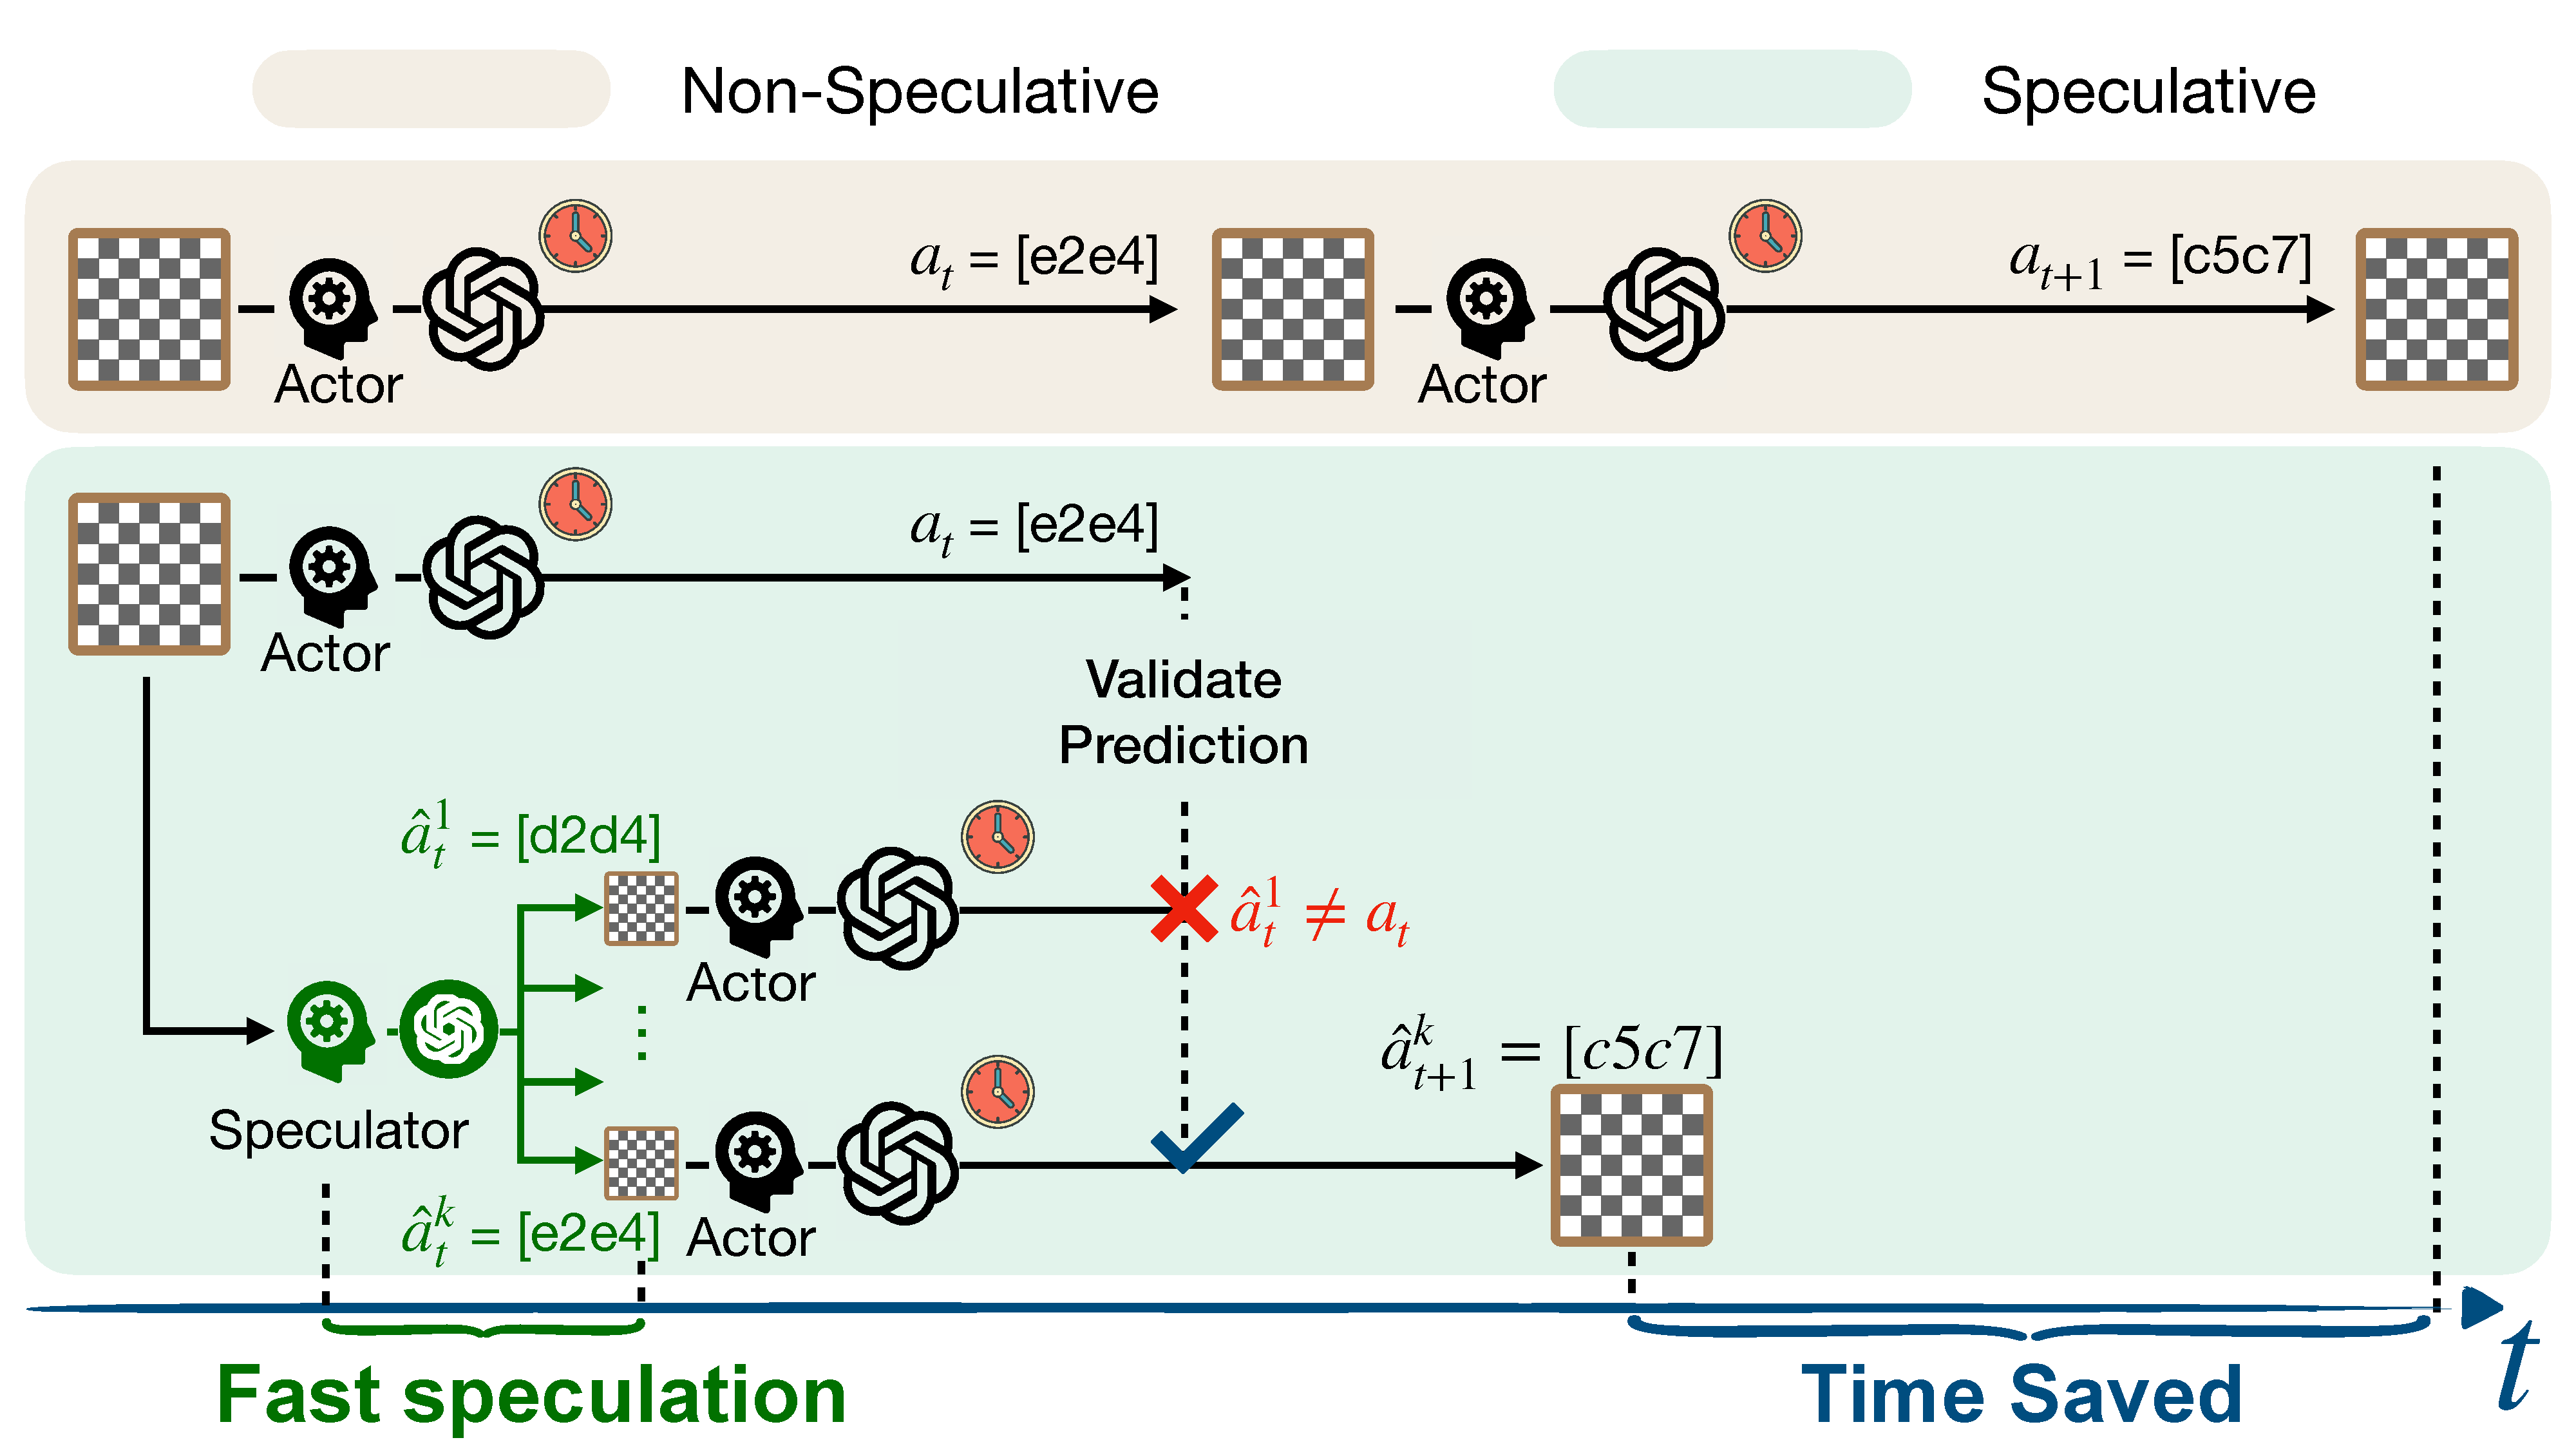
\includegraphics[width=0.9\linewidth]{figures/Speculative_figure_1.pdf}
    \caption{Illustration of our framework in a chess-playing environment. While the Actor issues an LLM call to decide the next move, the Speculator uses a faster model to guess it. These guesses enable parallel API calls for the next steps, and once a guess is verified, the system gains time through parallelization. The process runs in the backend, ensuring a lossless speedup for the user.}
    \label{fig:figure_1}
\end{figure}

% This design yields three practical acceleration modes:

% \begin{itemize}[leftmargin=*]
%     \item \emph{LLM-for-LLM} speculation: a fast model predicts the output (or sufficient control signals) of a slower, stronger model so the environment pipeline can keep moving without blocking on the validator.
%     \item \emph{LLM-for-tool} (or human) speculation: a model predicts likely API/human responses, enabling early environment interactions such as pre-issuing idempotent reads, warming caches, reserving items with TTLs, or staging purchases and forms pending confirmation.
%     \item \emph{Proactive action under deadline}: when the cost of inaction in the environment exceeds the expected penalty of a suboptimal move, a fast model takes a reversible or low-stakes action immediately (hold a seat, start a cancellable job, quickly adjust an OS policy), with later correction if needed.
% \end{itemize}

A key design goal is losslessness relative to the environment’s baseline semantics: speculative actions should not degrade final outcomes compared to a strictly sequential agent.
We achieve this with (a) semantic guards (actors confirm equivalence of state transitions before commit), (b) safety envelopes (only idempotent, reversible, or sandboxed speculative side effects), and (c) repair paths (rollback or compensating actions when a guess is rejected).
In many environments (e.g., web search, pre-checkout shopping carts, and OS-level operations in a sandbox) these patterns are natural and inexpensive to implement.


\textbf{Can we guess the next API calls of agents?} We show that, in practice, API intents can often be guessed with reasonable accuracy. In particular, we demonstrate speculative actions across four environments, each highlighting different aspects of agent latency:
\begin{itemize}[leftmargin=*]
    \item \textbf{Turn-based gameplay} (e.g., chess): the Speculator predicts the opponent's move while waiting for its turn.
See \cref{fig:figure_1}.
    \item \textbf{E-commerce}: while conversing with a shopper, the Speculator proactively infers the shopper's intent (e.g., returning an item), and triggers tool calls in advance (e.g., checking return eligibility).
    % \item \textbf{Web search \& question answering}
    \item \textbf{Multi-hop web search}: while awaiting results from slow external calls (e.g., Wikipedia), the Speculator can guess answers from its knowledge base, and execute subsequent search queries.
 
    % network-bound pipelines benefit from speculative query execution, snippet extraction, and prefetching.
    \item \textbf{Operating systems (lossy extension)}: speculative, reversible actions react immediately to workload and environment changes, boosting end-to-end performance while actors confirm.
\end{itemize}

% Across these settings, we observe substantial acceleration---up to 50\% accuracy in predicting the next API calls and 30\% end-to-end lossless speedup. These results are achieved with a simple implementation using single-step speculation, and can be improved upon performance can be further boosted with advanced techniques such as adaptive speculation.  Qualitatively, users experience truly interactive agents that feel responsive even when authoritative components are slow.

Across these settings, we observe substantially reduced latency, with up to 55\% accuracy in predicting the next API calls and 20\% end-to-end speedup.
These results are achieved with a simple single-step speculation, and can be improved by advanced techniques such as adaptive speculation. 

Finally, we give a cost-latency analysis that formally characterizes the tradeoff between speculating additional API calls and the resulting time savings.
We provide a theoretical baseline for choosing the speculative breadth, %and show that confidence-based selection can incur costs that grow substantially slower than naive linear scaling in the number of branches. 
and show that the cost incurred by confidence-based selection grows substantially slower than naively scaling the number of speculative branches. 
Furthermore, in our OS-tuning environment where losslessness is not required, cost and latency can actually both decrease. Our code is publicly available at \url{https://github.com/naimengye/speculative-action}.
% Qualitatively, users experience truly interactive agents that feel responsive even when authoritative components are slow.


% \input{sections/backup_related}
\subsection{Related Work}
\label{sec:related}
\paragraph{Speculative decoding and reasoning}
Our work is inspired by the use of speculative decoding in LLM inference. This technique accelerates autoregressive inference by using a small model to propose tokens which a larger target model verifies in batches, committing correct tokens and regenerating failures~\citep{leviathan2023fast,zhang2024beyond,chen2023acceleratinglargelanguagemodel}.
At the reasoning level, speculation has also been used to accelerate chain-of-thought~\citep{wang2025acceleratinglargelanguagemodel,wang2025efficientreasoningllmsspeculative,fu2025scaling}.
Our framework adopts the same speculate-verify pattern at the level of API calls.

\paragraph{Speculative planning for LLM agents}
More directly related are recent works on speculative planning for LLM-based agents~\citep{hua2024interactivespeculativeplanningenhance,guan2025dynamicspeculativeagentplanning}. 
\citet{hua2024interactivespeculativeplanningenhance} introduce interactive speculative planning, where a fast approximator proposes multi-step lookahead plans that are verified by a stronger model, with user interruption integrated. Their approach focuses on depth-oriented speculation along a single planning branch. Building on this, \citet{guan2025dynamicspeculativeagentplanning} propose an online reinforcement learning method to dynamically determine the number of future steps to speculate, optimizing a cost-latency tradeoff while maintaining lossless execution.

Our work differs along two dimensions. First, we generalize speculation beyond planning to the \emph{entire agentic environment}, including LLM calls, internal and external tool APIs, MCP-server interactions, and even human responses. This yields a unified framework for agentic speculation, particularly consistent with the emerging ``environment'' and MCP perspectives on agentic systems. Second, instead of depth-focused multi-step lookahead, we study a breadth-focused $k$-branch single-step strategy, where multiple actions are speculated in parallel at each step. We provide a cost-latency analysis for this scheme and derive closed-form expressions for expected time and token savings (Theorem~\ref{thm:cost-latency-tradeoff}). Section~\ref{sec:cost-latency} compares breadth- and depth-focused strategies under a unified analytical framework. While~\citet{guan2025dynamicspeculativeagentplanning} optimize depth dynamically, we characterize the optimal number of speculative branches per step as a function of predicted accuracy (Section~\ref{subsec:dynamic-speculation}).

% \paragraph{Speculative planning}
% More directly related are recent works on \emph{speculative planning} for LLM-based agents \citep{hua2024interactivespeculativeplanningenhance, guan2025dynamicspeculativeagentplanning}. In particular, \citet{hua2024interactivespeculativeplanningenhance} proposes a framework for interactive agent planning where user interaction and interruption are key components of the system.
% While our framework does not support user interaction, it generalizes speculations to the \textbf{entire agentic environment}:
% in addition to LLM calls, our framework also speculates internal and external tool APIs, MCP-server APIs, and even human responses. This yields a unified framework for agentic speculation, particularly consistent with the emerging ``environment'' and MCP perspectives on agentic systems.

% While \citet{hua2024interactivespeculativeplanningenhance} speculate using a depth-focused single-branch multi-step lookahead strategy, our framework uses a breadth-focused $k$-branch single-step search, where the Speculator explores $k$ speculative branches at each step in parallel.
% We give a cost-latency analysis for this generalized $k$-branch scheme and give a closed form for the expected time and token savings~\ref{thm:cost-latency-tradeoff}. We compare our breadth-focused strategy to a depth-focused one in Section~\ref{sec:cost-latency}.

% In concurrent work, \citet{guan2025dynamicspeculativeagentplanning} build on \citet{hua2024interactivespeculativeplanningenhance} with an online reinforcement learning framework to dynamically determine the number of steps to speculate,
% with each step still fixed to a single speculative branch.
% Our work explores optimization in the other dimension,
% where we give a technique to statically compute the optimal number of speculative branches per step based on a predicted accuracy~\ref{subsec:dynamic-speculation}


\paragraph{Speculation in systems and architecture}
Speculation is prominently used in computer architecture to increase parallelism
by executing instructions before their outcomes were resolved~\citep{tomasulo1967efficient} and 
rolling back when predictions were wrong~\citep{lam1992limits}. In light of security vulnerabilities that exploit microarchitectural speculative execution, \citep{mambretti2019speculator} developed Speculator to analyze CPU speculation behavior. 

Similar ideas arise in systems software as thread-level speculation, which parallelizes sequential code under assumed independence and rolls back upon detecting data dependencies or conflicts~\citep{10.1145/2938369}. Recently, \citep{liargkovas2023shell} explored the use of tracing and containment to speculatively but safely run shell scripts out of order. Beyond traditional systems context, speculative techniques have also been used to parallelize otherwise sequential security checks~\citep{nightingale2008parallelizing},test configuration changes in isolation ~\citep{su2007autobash}, and accelerate policy simulation in supply chain optimization~\citep{farias2024speeding}.



\section{Framework}
\label{framework}
An agentic system is modeled as a Markov Decision Process (MDP) $(s_{t}, a_{t})$, where $s_{t}$ denotes the state and $a_{t}$ the agent’s action at step $t$. 
This model admits considerable flexibility: an action may represent a chatbot response, a tool call, or a button clicked by a computer-use agent, among others.  

From a systems perspective, we model each action in an agentic system as an \emph{API call}, which may block execution until a response is returned. This abstraction offers two key advantages: (1) it precisely defines what constitutes an action, and (2) it provides a unified framework for optimizing system latency, as we will see shortly.
Notably, this perspective aligns with the recent development of MCP servers for agentic systems \citep{anthropic2024model}.

Formally, at each step $t$, the policy $\pi$ maps the current state $s_{t}$ to an API call:
\[
(h_{t}, q_{t}) \gets \pi(s_{t}),
\]
where $h_{t}$ specifies the target API to invoke and $q_{t}$ its associated parameters. We write
\[\bar a_t \leftsquigarrow h_t(q_t)\qquad a_t \gets \mathrm{await}(\bar a_t)\] 
to denote an asynchronous API invocation that
returns a \emph{future} (a pending action), and the await for when the response actually arrives. We use the bar notation (e.g., $\bar a$) for futures and
a cache $\mathcal C:(h,q)\mapsto \bar a$ that maps an API call specifier to its pending response. The left squiggly arrow indicates an asynchronous call with non-negligible delay.

The system subsequently transitions to the next state via a transition function $f$: $
s_{t+1} \gets f(s_{t}, a_{t}).$
As a concrete example, consider chess: the policy $\pi$ determines how to construct the prompt 
based on the current board state, $a_{t}$ corresponds to the move proposed by the LLM’s response, 
and $f$ updates the board configuration accordingly. Note that the LLM call is the API, its \textit{response} is the move $a_t$. 


This formulation subsumes a broad range of realizations:
\begin{itemize}[leftmargin=*]
    \item \textbf{LLM calls:} each invocation of an LLM within the agent can be treated as an action.
    \item \textbf{Tool / MCP server calls:} each actual call for internal/external tools is treated as an action: e.g., terminal access, web search, deep research APIs, weather APIs, or browser-use MCPs.
    \item \textbf{Human-as-an-API calls:} furthermore, human responses themselves can be abstracted as API calls, often incurring even longer latencies than automated tools.
\end{itemize}

Given this abstraction, the fundamental bottleneck in executing agentic systems becomes apparent: each API call must complete before the next can be issued. To break this sequential dependency, we propose to \textbf{speculate a set of API responses} $\{\hat{a}_{t}\}$ using a faster model while waiting for the true response $a_{t}$. This enables speculative API calls for step $t+1$ to be launched in parallel. At time $t$, if the API call $(h_t, q_t)$ can be found in the cache (cache hit), the system can skip the actual invocation and only wait for the pending action corresponding to this call to return (if not already returned). Formally, the algorithm is specified in \cref{alg:speculative-k}. 


% \begin{algorithm}
% \caption{Speculative actions with $k$-way parallel next calls}
% \label{alg:speculative-k}
% \begin{algorithmic}[1]
% \Require Initial state $s_0$, horizon $T$, transition $f$, policy $\pi$, predictor $\hat g$, cache $\mathcal{C}$
% \For{$t = 0$ to $T-1$}
%     \State \textbf{Policy:} $(h_t,q_t) \gets \pi(s_t)$
%     \If{$(h_t,q_t) \in \mathcal{C}$} \Comment{Cache hit}
%         \State $a_t \gets \mathcal{C}[(h_t,q_t)]$
%         \State $s_{t+1} \gets f\big(s_t,a_t\big)$
%         \State \textbf{continue}
%     \EndIf
%     \State \textbf{Actor:} Issue real request (non-blocking): $a_t \leftsquigarrow h_t(q_t)$
%     \State \textbf{Speculator:} $ \{\hat a_t^{(i)}\}_{i=1}^k \gets \hat g(s_t,(h_t,q_t))$
%     \Comment{Actor and speculator run in parallel}
%     \For{$i=1$ to $k$} \Comment{One-step speculative rollout per guess}
%         \State $\hat s_{t+1}^{(i)} \gets f\big(s_t, \hat a_t^{(i)}\big)$
%         \State $(\hat{h}_{t+1}^{(i)},\hat{q}_{t+1}^{(i)}) \gets \pi(\hat s_{t+1}^{(i)})$
%         \State Issue real request (non-blocking): $\hat{a}_{t+1}^{(i)} \leftsquigarrow \hat{h}_{t+1}^{(i)}\!\big(\hat{q}_{t+1}^{(i)}\big)$\\
%         \hspace{155pt}  $\mathcal{C}[(\hat{h}_{t+1}^{(i)},\hat{q}_{t+1}^{(i)})] \gets \hat{a}_{t+1}^{(i)}$
%         \Comment{On arrival, cache speculation}
%     \EndFor
%     \State \textbf{Wait for $a_t$ from either Actor or cache $C$}
%     \State $s_{t+1} \gets f\big(s_t,a_t\big)$
% \EndFor
% \end{algorithmic}
% \end{algorithm}



\begin{algorithm}
\caption{Speculative actions with $k$-way parallel next calls}
\label{alg:speculative-k}
\begin{algorithmic}[1]
\Require Initial state $s_0$, horizon $T$, transition $f$, policy $\pi$, predictor $\hat g$, cache $\mathcal{C}$. We use $\bar{a}$ to denote pending action.
\For{$t = 0$ to $T-1$}
    \State \textbf{Policy:} $(h_t,q_t) \gets \pi(s_t)$
    \If{$(h_t,q_t) \in \mathcal{C}$} \Comment{Cache hit}
        \State $\bar{a}_t \gets \mathcal{C}[(h_t,q_t)]$
        \State $a_t \gets \text{await}(\bar{a}_t)$
        \Comment{Await pending action if not returned already}
        \State $s_{t+1} \gets f\big(s_t,a_t\big)$
        \State \textbf{continue}
    \EndIf
    \State \textbf{Actor:} Issue real request (returns future): $\bar{a}_t \leftsquigarrow h_t(q_t)$
    \State \textbf{Speculator:} 
    $ \{\hat{a}_t^{(i)}\}_{i=1}^k \gets \text{await}(\hat g(s_t,(h_t,q_t)))$
    \Comment{Actor and speculator run in parallel}
    \For{$i=1$ to $k$} \Comment{One-step speculative rollout per guess}
        \State $\hat s_{t+1}^{(i)} \gets f\big(s_t, \hat a_t^{(i)}\big)$
        \State $(\hat{h}_{t+1}^{(i)},\hat{q}_{t+1}^{(i)}) \gets \pi(\hat s_{t+1}^{(i)})$
        \State \textbf{Pre-launch}: $\bar{\hat{a}}_{t+1}^{(i)} \leftsquigarrow \hat{h}_{t+1}^{(i)}\!\big(\hat{q}_{t+1}^{(i)}\big)$
        \Comment{Return pending action, hence non-blocking}
        \State \hspace{73pt}  $\mathcal{C}[(\hat{h}_{t+1}^{(i)},\hat{q}_{t+1}^{(i)})] \gets \bar{\hat{a}}_{t+1}^{(i)}$
        \Comment{Cache speculative pending actions}
    \EndFor
    \State \textbf{Wait for resolved $a_t$ from Actor:} $a_t\gets \text{await}(\bar{a}_t)$
    \State $s_{t+1} \gets f\big(s_t,a_t\big)$
\EndFor
\end{algorithmic}
\end{algorithm}


% \begin{algorithm}
% \caption{Speculative actions with $k$-way parallel next calls}
% \label{alg:speculative-k}
% \begin{algorithmic}[1]
% \Require Initial state $s_0$, horizon $T$, transition $f$, policy $\pi$, predictor $\hat g$, cache $\mathcal{C}$. We use $\bar{b}$ to denote pending response of the API call.
% \For{$t = 0$ to $T-1$}
%     \State \textbf{Policy:} $q_t \gets \pi_1(s_t)$
%     \If{$q_t \in \mathcal{C}$} \Comment{Cache hit}
%         \State $\bar{b}_t \gets \mathcal{C}[q_t]$
%         \State $b_t \gets \text{await}(\bar{b}_t)$
%         \Comment{Await pending action if not returned already}
%         \State $a_t \gets \pi_2(b_t, s_t)$
%         \State $s_{t+1} \gets f\big(s_t,a_t\big)$
%         \State \textbf{continue}
%     \EndIf
%     \State \textbf{Actor:} Issue real request: $\bar{b}_t \leftsquigarrow \text{call\_API}(q_t)$
%     \Comment{Return pending response, non-blocking}
%     \State \textbf{Speculator:} 
%     $\{\hat{\bar b}_t^{(i)}\}_{i=1}^k \gets \text{call\_API}(\hat g(s_t))$
%     \Comment{Actor and speculator run in parallel}
%     \For{$i=1$ to $k$} \Comment{One-step speculative rollout per guess}
%        \State $\hat{b}_t^{(i)}\gets\text{await}\left(\hat{\bar b}_t^{(i)}\right)$
%         \State $\hat{a}_t^{(i)}\gets\pi_2(s_t,\hat{b}_t^{(i)})$
%         \State $\hat s_{t+1}^{(i)} \gets f\big(s_t, \hat a_t^{(i)}\big)$
%         \State $\hat{q}_{t+1}^{(i)} \gets \pi(\hat s_{t+1}^{(i)})$
%         \State Issue real request: $\bar{\hat{b}}_{t+1}^{(i)} \leftsquigarrow \text{call\_API}\big(\hat{q}_{t+1}^{(i)}\big)$
%         \Comment{Return pending action, hence non-blocking}
%         \State \hspace{73pt}  $\mathcal{C}[(\hat{q}_{t+1}^{(i)})] \gets \bar{\hat{b}}_{t+1}^{(i)}$
%         \Comment{Cache speculative pending actions}
%     \EndFor
%     \State \textbf{Wait for response $b_t$ from Actor:} $b_t\gets \text{await}(\bar{b}_t)$
%     \State $a_t\gets\pi_2(b_t,s_t)$
%     \State $s_{t+1} \gets f\big(s_t,a_t\big)$
% \EndFor
% \end{algorithmic}
% \end{algorithm}


The resulting speedup relies on two key assumptions:  

% \begin{assumption}
% \label{assum:guessing-accuracy}
% The speculative model is able to guess $(h_{t+1}, q_{t+1})$ with non-zero probability.
% \end{assumption}

\begin{assumption}[Speculation accuracy]\label{assum:guessing-accuracy}
The speculative model $\hat g$ guesses the current-step response $a_t$ accurately enough that
the implied next call $(h_{t+1},q_{t+1})=\pi(f(s_t,\hat a_t))$ matches the true next call with probability $p>0$.
\end{assumption}


As shown later, this often holds in practice because API responses are typically predictable.  

\begin{assumption}[Concurrent, reversible pre-launch]\label{assum:concurent-API}
Multiple API calls can be launched concurrently, and pre-launched calls that do not correspond to
the realized trajectory have no externally visible side effects (or can be rolled back).
\end{assumption}


In practice, this assumption is satisfied under modest traffic for many external APIs (e.g., web search, OpenAI LLM queries, email lookups). For self-hosted LLMs, concurrent calls also incur only minimal additional cost due to continuous batching.  

We can then establish the following result (with proof deferred to the Appendix~\ref{app:proof}).  


\begin{proposition}
\label{thm:improvement}
Under Assumptions \ref{assum:guessing-accuracy}--\ref{assum:concurent-API}, suppose at each step
the speculative branch implies the \emph{correct next call} $(h_{t+1},q_{t+1})$ with probability $p$, independently across $t\in[1,T-1]$. Let the latency of $\hat{g}$ be $\mathrm{Exp}(\alpha)$ and the latency of the actual API call be $\mathrm{Exp}(\beta)$ with $\beta < \alpha$. All latencies and guesses occur independently. Assume the transition $f$ and API parameter construction $\pi$ are negligible. Then the ratio between the expected runtime of \cref{alg:speculative-k}, denoted $\E[T_{\mathrm{s}}]$, and the expected runtime of sequential execution, $\E[T_{\mathrm{seq}}]$, is
{\small\begin{align*}
    \frac{E[T_{\mathrm{s}}]}{E[T_{\mathrm{seq}}]}
    \;=\;
    1 - \frac{1}{T}\frac{\alpha}{\alpha+\beta}\left[\frac{(T-1)p(k)}{1+p(k)}+\frac{p(k)^2}{(1+p(k))^2} - \frac{p(k)^2}{(1+p(k))^2}(-p(k))^{T-1}\right]\xrightarrow{\;\;T\to\infty\;\;}
    1-\frac{p(k)}{1+p(k)}\cdot\frac{\alpha}{\alpha+\beta}
\end{align*}}
where $p(k) = 1- (1-p)^k$ denotes the probability of at least one of the $k$ speculations hit.
\end{proposition}
\cref{thm:improvement} suggests the end-to-end latency reduction has an upper bound of 50\%, occurring when $p=1$ and $\alpha=\infty$.This can be further improved by the multi-step extension below.  

\paragraph{Extension} \cref{alg:speculative-k} is only a simple demonstration of the idea. For example, one can naturally extend \cref{alg:speculative-k} to \emph{multi-step speculation}, where the Speculator predicts not only the next, but $s$ steps ahead. This yields a tree structure with deeper rollouts. This can be further combined with \emph{adaptive speculation}: instead of generating $k$ guesses for $a_t$ uniformly, the Speculator also estimates confidence for each guess (e.g., via prompting LLMs or uncertainty-quantification methods), this is explored in Section\ref{sec:cost-latency}. The most promising branches can then be expanded in a beam-search–like manner. Together, these ideas highlight the richness of speculative actions. Despite \cref{alg:speculative-k}'s simplicity, the results from the four use cases in the following sections are already highly promising.

% We defer a detailed discussion to the Appendix,

\paragraph{Side effects and safety}
Speculation executes a hypothesized next action $\hat a_{t+1}$ that may be wrong, so safety requires the ability to simulate first and then commit or roll back. In domains like chess, rollback is trivial; in others, overwrite is easy (e.g., OS tuning). But many systems involve irreversible or externally visible effects (e.g., deleting records, placing orders), where naive speculation is harmful. Thus, speculation must be limited to cases where mispredictions are reversible, via forking, snapshot restoration, or roll-forward repair (e.g., refund/replace).
\vspace{-10pt}
\section{Environments}
We now instantiate speculative actions in three environments---chess, e-commerce dialogue, and multi-hop web search---chosen 
to stress distinct latency bottlenecks (reasoning, tool/API round trips, and information retrieval).
We pair a fast Speculator with a slow Actor and implement Algorithm~\ref{alg:speculative-k}. 

% under lossless, as-if-sequential semantics, 
% committing only when validated and discarding mismatches, and we report prediction accuracy and end-to-end time saved.

\label{sec:environments}
\subsection{Chess Environment}
\label{subsec:chess}
\begin{wrapfigure}{r}{0.5\columnwidth}
    \centering%
    \vspace{-15pt}
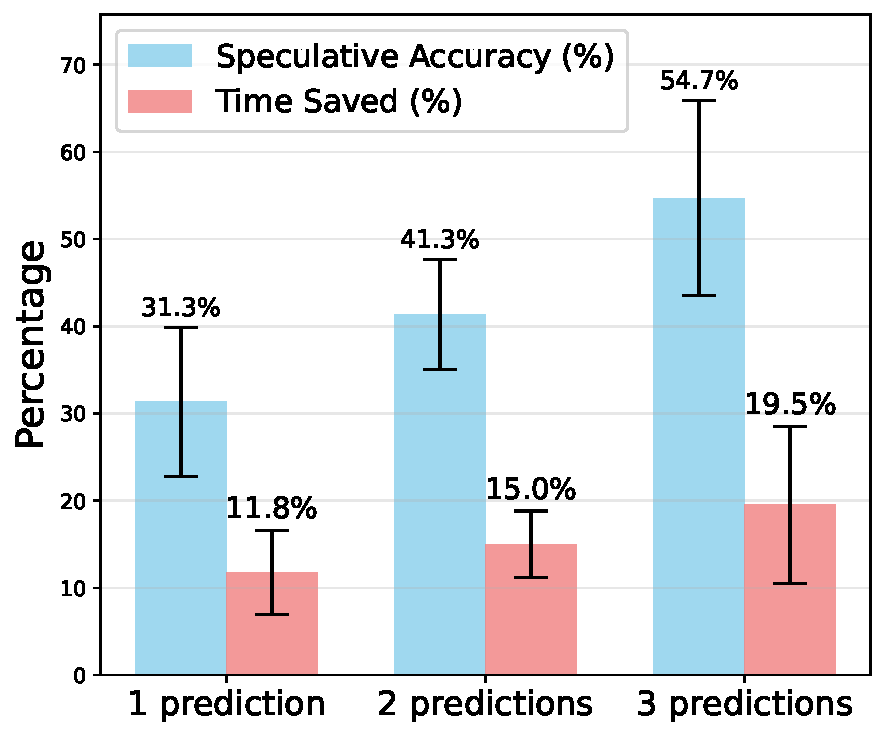
\includegraphics[width=0.85\linewidth]{figures/chess/combined_bar_plots.pdf}
  \caption{Percentage of time saved and percentage of correct predictions across $5$ runs at $30$ steps.}
  \label{fig:chess_bar_plots}
  \vspace{-15pt}
\end{wrapfigure}
We demonstrate the effectiveness of our  framework in the context of multi-agent gameplay, focusing on chess as a canonical turn-based example. In standard play, analysis is strictly sequential: each player begins analysis only \textit{after} the opponent has completed their turn. This serialization introduces substantial idle time. Particularly when both players rely on computationally intensive reasoning models, a single game can stretch to hours of wall-clock time. Our framework relaxes this constraint through speculative parallel analysis, allowing players to anticipate and prepare for likely opponent moves in advance. We show that this results in significant reductions in overall game duration.
% This strict serialization makes chess an ideal testbed for demonstrating how speculation can parallelize inherently sequential interactions.

\subsubsection{Implementation}
We implement our framework on top of TextArena \citep{guertler2025textarena}, which provides a standardized gameplay interface for LLM-driven agents.

\paragraph{Speculative pipeline} At turn $t$, the game state $s_t$ corresponds to the current board position. The in-turn player issues an API call $h_t$ with parameter $q_t$ constructed from $s_t$ together with a reasoning-eliciting prompt. At this point, player $P$ is to move, and player $Q$ awaits. Proceeds as follows:
\begin{itemize}[leftmargin=*]
    \item Current in-turn player $P$: the player receives $s_t$, makes an API call $h_t$ to the agent with parameter $q_t = (s_t, \text{prompt})$. This API call returns the next move $a_t = h(q_t)$, typically with high latency due to deep and extensive reasoning.
    \item Other out-of-turn player $Q$:
    \begin{enumerate}
        \item \textbf{Prediction phase} The Speculator also receives the board state $s_t$ and issues an API call $\hat{h}_t$, using a prompt optimized for speed rather than depth. It returns the top-$k$ move predictions $\hat{a}_t^{(1)}, \hat{a}_t^{(2)}, \dots, \hat{a}_t^{(k)}$, ordered by confidence.
        \item \textbf{Parallel computation} For each predicted move $\hat{a}_t^{(i)}$, the out-of-turn player $Q$ immediately launches a process analyzing a next move $\hat{a}_{t+1}^{(i)} = h_{t+1}(\hat{s}_{t+1}, {prompt})$ for $i \in \{1, \ldots, k\}$, where $ \hat{s}_{t+1}^{(i)} = f(s_t,\hat{a}_t^{(i)})$ denotes the next state resulting from applying the predicted action $\hat{a}_t^{(i)}$ to $s_t$. 
        \item \textbf{Validation} When the current in-turn player $P$ finishes reasoning and returns its move $a_t$, we immediately check whether it matches any of the predicted moves $\hat{a}_t^{(1)}, \hat{a}_t^{(2)}, \dots, \hat{a}_t^{(k)}$. 
        \item \textbf{Commit or restart} If a match exists, we commit to the corresponding speculative branch, advancing directly to $s_{t+1} = f(s_t, a_t)$. The game thus skips ahead, terminating other threads. If no match exists, we discard all speculative branches and continue with $Q$’s regular move computation $a_{t+1} = h_{t+1}(f(s_{t},a_t),\text{prompt})$. 
    \end{enumerate}
\end{itemize}

This pipeline is \textit{lossless}: the final trajectory remains identical to non-speculative play, but time is saved through parallelized reasoning.

\paragraph{Agent Configuration} We find that using the same model for both Speculator and Actor, but with different prompts, maximizes prediction accuracy while keeping speculation fast. Accordingly, in our experiments, the Actor is instantiated with GPT-5 with high reasoning effort; and the Speculator is instantiated with GPT-5 configured with low reasoning effort and a specialized system prompt designed for rapid move prediction rather than exhaustive analysis.

\subsubsection{Results}
We evaluate our framework in terms of both time saved and prediction accuracy. We track two metrics: (i) prediction accuracy: the fraction of rounds in which any speculative prediction matches the actual move; and (ii) time saved:  $(T_{seq}-T_{s})/T_{seq}$, where $T_{s}$ and $T_{seq}$ denote speculative and sequential execution times, respectively.

\textbf{More predictions improve time savings and accuracy.}
Figure~\ref{fig:chess_bar_plots} reports results over 30~steps. Our framework consistently reduces execution time, with larger savings as the number of speculative predictions increases. Across 5 runs, using 3 predictions yields an average time saving of $19.5\%$ with an average prediction accuracy of $54.7\%$.

\textbf{Randomness of agent call in gameplay.}
% The variance in Figure~\ref{fig:chess_bar_plots} reflects realistic system and gameplay dynamics that arise from live API calls. Even with correct predictions, time savings vary: when the resulting position admits an obvious response, little acceleration occurs, as computation would have been fast regardless. Significant gains arise only when predictions lead to positions requiring deep analysis.
The variance in Figure~\ref{fig:chess_bar_plots} reflects realistic latency fluctuations from live API calls. Even with correct predictions, speedups vary: if the resulting position is trivial, little acceleration is realized; large gains occur only when predictions lead to positions requiring deep analysis.
%
In addition, API latency itself is inherently stochastic. Backend load fluctuations (e.g., concurrent traffic to the model provider) can cause the same API call with different latency across runs. 
Consequently, measured latency reductions exhibit natural variability and are not perfectly reproducible.
\subsection{E-Commerce Environment}
\label{subsec:ecommerce}
Beyond competitive gameplay, customer-agent interactions in e-commerce provide a real-world setting where latency significantly impacts user experience. In a typical workflow, the customer submits a query through a chat interface and waits while the agent sequentially invokes multiple API calls—for example, processing a return may involve retrieving order information, validating eligibility for each item, and initiating the return. These chained calls can introduce substantial delay. By contrast, if some API calls are correctly speculated and executed in advance, the agent can return results immediately once the query arrives, making the interaction feel seamless. We evaluate this setting using the retail environment from \emph{$\tau$-bench}~\citep{yao_Taubench_2024}.
\subsubsection{Experimental Setup}
\paragraph{Speculative pipeline} 
In this scenario, the current state $s_t$ is defined as the conversation history up to turn $t$, and $h_t$ are the API calls required to answer the user's query (eg. get\_user\_details, get\_order\_details). Our Speculator will predict
\begin{enumerate}
    \item The user’s query $\hat{a}_t$;
    \item The target API calls and their corresponding parameters $(\hat{h}_{t+1}^{(i)}, \hat{q}_{t+1}^{(i)})$ for $i \in \{1, ..., k\}$, conditioned on the current state $s_t$ and the predicted user's query from step 1. Since the number of API calls for each turn is not fixed, the Speculator must also predict $k$.
\end{enumerate}
% Our framework executes as follows, 
% \begin{itemize}[leftmargin=*]
%     \item \textbf{Prediction phase}. While the user is composing their query, the Speculator attempts to predict: i) The user’s query $\hat{a}_t$; ii) The target API calls and their corresponding parameters $(\hat{h}_{t+1}^i, \hat{q}_{t+1}^i)$ for $i \in \{1, ..., k\}$, conditioned on the current state $s_t$ and the predicted user's query from step 1. Since the number of API calls for each turn is not fixed, the Speculator also determines $k$.
%     \item \textbf{Validation}. Once the user submits their actual query, the Actor determines the required ground-truth API calls $(h_{t+1}, q_{t+1})$, the system validates whether any speculative calls match.
%     \item \textbf{Commit or discard}. If one or more speculative calls match the required ground-truth API calls, their results are immediately committed, thereby eliminating latency. Otherwise, speculative calls are safely discarded and execution proceeds normally.
% \end{itemize}
\vspace{-5pt}

% \paragraph{Agent configuration} We test various models as Speculator: OpenAI GPT models (gpt-5-nano, gpt-5-mini, gpt-5) and Google Gemini models (gemini-2.5-flash) with different reasoning budgets (1024, 2048, 4096 tokens).
% Prior work~\cite{jiang-etal-2023-llm, chen_LLMEnsemble_2025} shows that heterogeneous LLM ensembles often outperform individual models, and multiple models can execute in parallel under the same time budget. Motivated by these findings, we evaluate two Speculator configurations: (i) a \emph{single-model} setting, where speculation relies on one model, and (ii) a \emph{multi-model} setting, where models with comparable capacity and reasoning budgets run in parallel (i.e., gpt-5-nano with low-budget Gemini, gpt-5-mini with medium-budget Gemini, and gpt-5 with high-budget Gemini). Their predictions are then aggregated into a shared candidate set of speculative actions. At runtime, when the user simulator provides the actual utterance, the Actor compares the speculative API calls with the ground-truth APIs. Correct predictions are committed immediately, eliminating latency, while incorrect predictions are safely discarded without affecting correctness.
\paragraph{Agent configuration}
\begin{wrapfigure}{r}{0.45\columnwidth}
    \centering
    \vspace{-15pt}
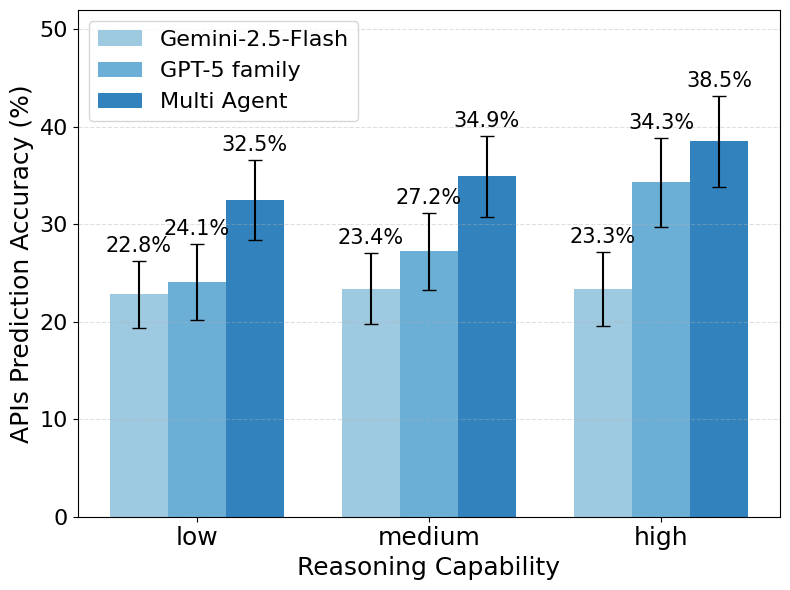
\includegraphics[width=0.85\linewidth]{figures/ecommerce/pred_acc_error_bar.png}
    \caption{APIs prediction accuracy across various Speculator models. %with various reasoning capability.
    }
    \label{fig:pred_acc}
    \vspace{-15pt}
\end{wrapfigure}
We evaluate multiple Speculator models, including OpenAI GPT variants (gpt-5-nano, gpt-5-mini, gpt-5) and Google Gemini (gemini-2.5-flash) under different reasoning budgets (1024/2048/4096 tokens). Motivated by prior work where heterogeneous LLM ensembles outperform single models~\citep{jiang-etal-2023-llm, chen_LLMEnsemble_2025}, we consider two configurations: (i) a \emph{single-model} Speculator, and (ii) a \emph{multi-model} Speculator, where comparable models run in parallel (e.g., gpt-5-nano with low-budget Gemini, gpt-5-mini with medium-budget Gemini). Their outputs are aggregated into a shared pool of candidate speculative actions.

At runtime, once the user simulator reveals the ground-truth utterance, the Actor validates the speculative API calls: correct predictions are committed immediately (eliminating latency), while incorrect ones are discarded without affecting correctness.
\paragraph{Evaluation} 
We evaluate performance using \textbf{APIs prediction accuracy}, defined as the fraction of speculative API calls that match the ground-truth APIs required to resolve the user’s query. This metric directly reflects the proportion of turns in which the user receives an immediate response, without waiting for API execution: higher prediction accuracy translates into greater time savings. 


% Surface-form mismatches in user utterances are disregarded, as responsiveness is determined solely by the correctness of API calls rather than by linguistic variation.

%predicted and true queries share intent (e.g., “I confirm I’d like to return the headphones and smart watch” vs. “Yup, go ahead.”).
% (ii) \textbf{Cost}, measured as cumulative time and price for model invocations and tool interactions. Because raw throughput and latency vary across deployment settings, we normalize cost statistics using empirical measurements reported in~\cite{}.
\subsubsection{Results}
Figure~\ref{fig:pred_acc} shows that between 22\% and 38\% of API calls are correctly predicted by the Speculator. Accuracy improves with stronger models and the multi-agent configuration consistently outperforms single-model speculation. Importantly, low-budget models speculate in only 2–3 seconds (per the LLM API providers leaderboard\footnote{\url{https://artificialanalysis.ai/leaderboards/providers}}), well below the average user typing time of about 30 seconds (assuming 40 words per minute). This means that in roughly one third of turns, the agent can respond faster than sequential execution, without waiting for API execution. 
% These results demonstrate that speculation can transform user experience from perceptibly delayed to effectively real-time in tool-heavy environments.


% The time cost is calculated based on the LLM API providers Leaderboard \footnote{\url{https://artificialanalysis.ai/leaderboards/providers}}, consists of latency (i.e., Time to First Token) and output response time (i.e., output tokens per second multiply by the number of output tokens). The dashed vertical line represents average user typing time, estimated as 40 words per minute multiplied by the average number of words per turn in the tasks. At this threshold, the multi-agent setting achieves approximately 34\% prediction accuracy, meaning that in over one-third of cases the agent can return an immediate response without waiting for API execution. This demonstrates that speculation can transform user experience from perceptibly laggy to effectively real-time in tool-heavy environments.


% \kostis{Start with the most important observation: Speculation accelerates things!!! Then go into the secondary budgetary/accuracy observations and trade-offs.}

% Overall, we observe three consistent trends. First, increasing the reasoning budget within the same model family leads to higher prediction accuracy (Figure~\ref{fig:gemini}), reflecting the benefit of additional compute for more precise intent prediction. Second, larger models within the same family achieve systematically better accuracy (Figure~\ref{fig:gpt5}), confirming the expected scaling advantage. Third, the multi-model speculative setting significantly boosts accuracy compared to single-model speculation, suggesting that results from different rounds or model variants complement each other and reduce coverage gaps. These gains, however, come with associated costs. Larger or more compute-intensive models incur higher latency and generation time, as well as increased monetary cost. Figures~\ref{fig:time} and~\ref{fig:price} make these trade-offs explicit: accuracy improves steadily with model scale and budget, but at the expense of both runtime and price.

% \begin{figure}[t]
%   \centering
%   \resizebox{0.8\textwidth}{!}{% <-- scale entire block to 90% of textwidth
%     \begin{minipage}{\textwidth}
%       \centering
%       % Row 1
%       \begin{subfigure}[t]{0.48\textwidth}
%         \includegraphics[width=\linewidth]{figures/ecommerce/figure_gpt5.png}
%         \caption{}
%         \label{fig:gpt5}
%       \end{subfigure}\hfill
%       \begin{subfigure}[t]{0.48\textwidth}
%         \includegraphics[width=\linewidth]{figures/ecommerce/figure_gemini.png}
%         \caption{}
%         \label{fig:gemini}
%       \end{subfigure}

%       \vspace{0.5em}

%       % Row 2
%       \begin{subfigure}[t]{0.48\textwidth}
%         \includegraphics[width=\linewidth]{figures/ecommerce/figure_time.png}
%         \caption{}
%         \label{fig:time}
%       \end{subfigure}\hfill
%       \begin{subfigure}[t]{0.48\textwidth}
%         \includegraphics[width=\linewidth]{figures/ecommerce/figure_price.png}
%         \caption{}
%         \label{fig:price}
%       \end{subfigure}
%     \end{minipage}
%   }
%   \caption{(a) Accuracy of the GPT-5 family with varying output lengths; dashed line indicates equivalent time cost under parallel execution. (b) Accuracy of the Gemini-2.5-flash family with varying output lengths; dashed line again marks the parallel cost threshold. (c) Accuracy–speculative time cost trade-off across models, where time is computed as average model latency plus token throughput; dashed line shows average user typing time. (d) Accuracy–price trade-off across models, reflecting the monetary cost of speculative execution.\kostis{MUCH MUCH bigger fonts and thicker lines please.}}
%   \label{fig:ecommerce}
% \end{figure}

% \begin{figure}[t]
%   \includegraphics[width=\columnwidth]{figures/ecommerce/figure_gpt5.png}
%   \caption{A figure with a caption that runs for more than one line.
%     Example image is usually available through the \texttt{mwe} package
%     without even mentioning it in the preamble.}
%   \label{fig:experiments}
% \end{figure}

% \begin{figure}[t]
%   \includegraphics[width=\columnwidth]{figures/ecommerce/figure_gemini.png}
%   \caption{A figure with a caption that runs for more than one line.
%     Example image is usually available through the \texttt{mwe} package
%     without even mentioning it in the preamble.}
%   \label{fig:experiments}
% \end{figure}

% \begin{figure}[t]
%   \includegraphics[width=\columnwidth]{figures/ecommerce/figure_time.png}
%   \caption{A figure with a caption that runs for more than one line.
%     Example image is usually available through the \texttt{mwe} package
%     without even mentioning it in the preamble.}
%   \label{fig:experiments}
% \end{figure}

% \begin{figure}[t]
%   \includegraphics[width=\columnwidth]{figures/ecommerce/figure_price.png}
%   \caption{A figure with a caption that runs for more than one line.
%     Example image is usually available through the \texttt{mwe} package
%     without even mentioning it in the preamble.}
%   \label{fig:experiments}
% \end{figure}




\subsection{HotpotQA Environment}
\label{subsec:hotpotqa}
% \begin{figure}[h]
% \end{figure}
\begin{wrapfigure}{r}{0.45\columnwidth}
\vspace{-10pt}
    \centering
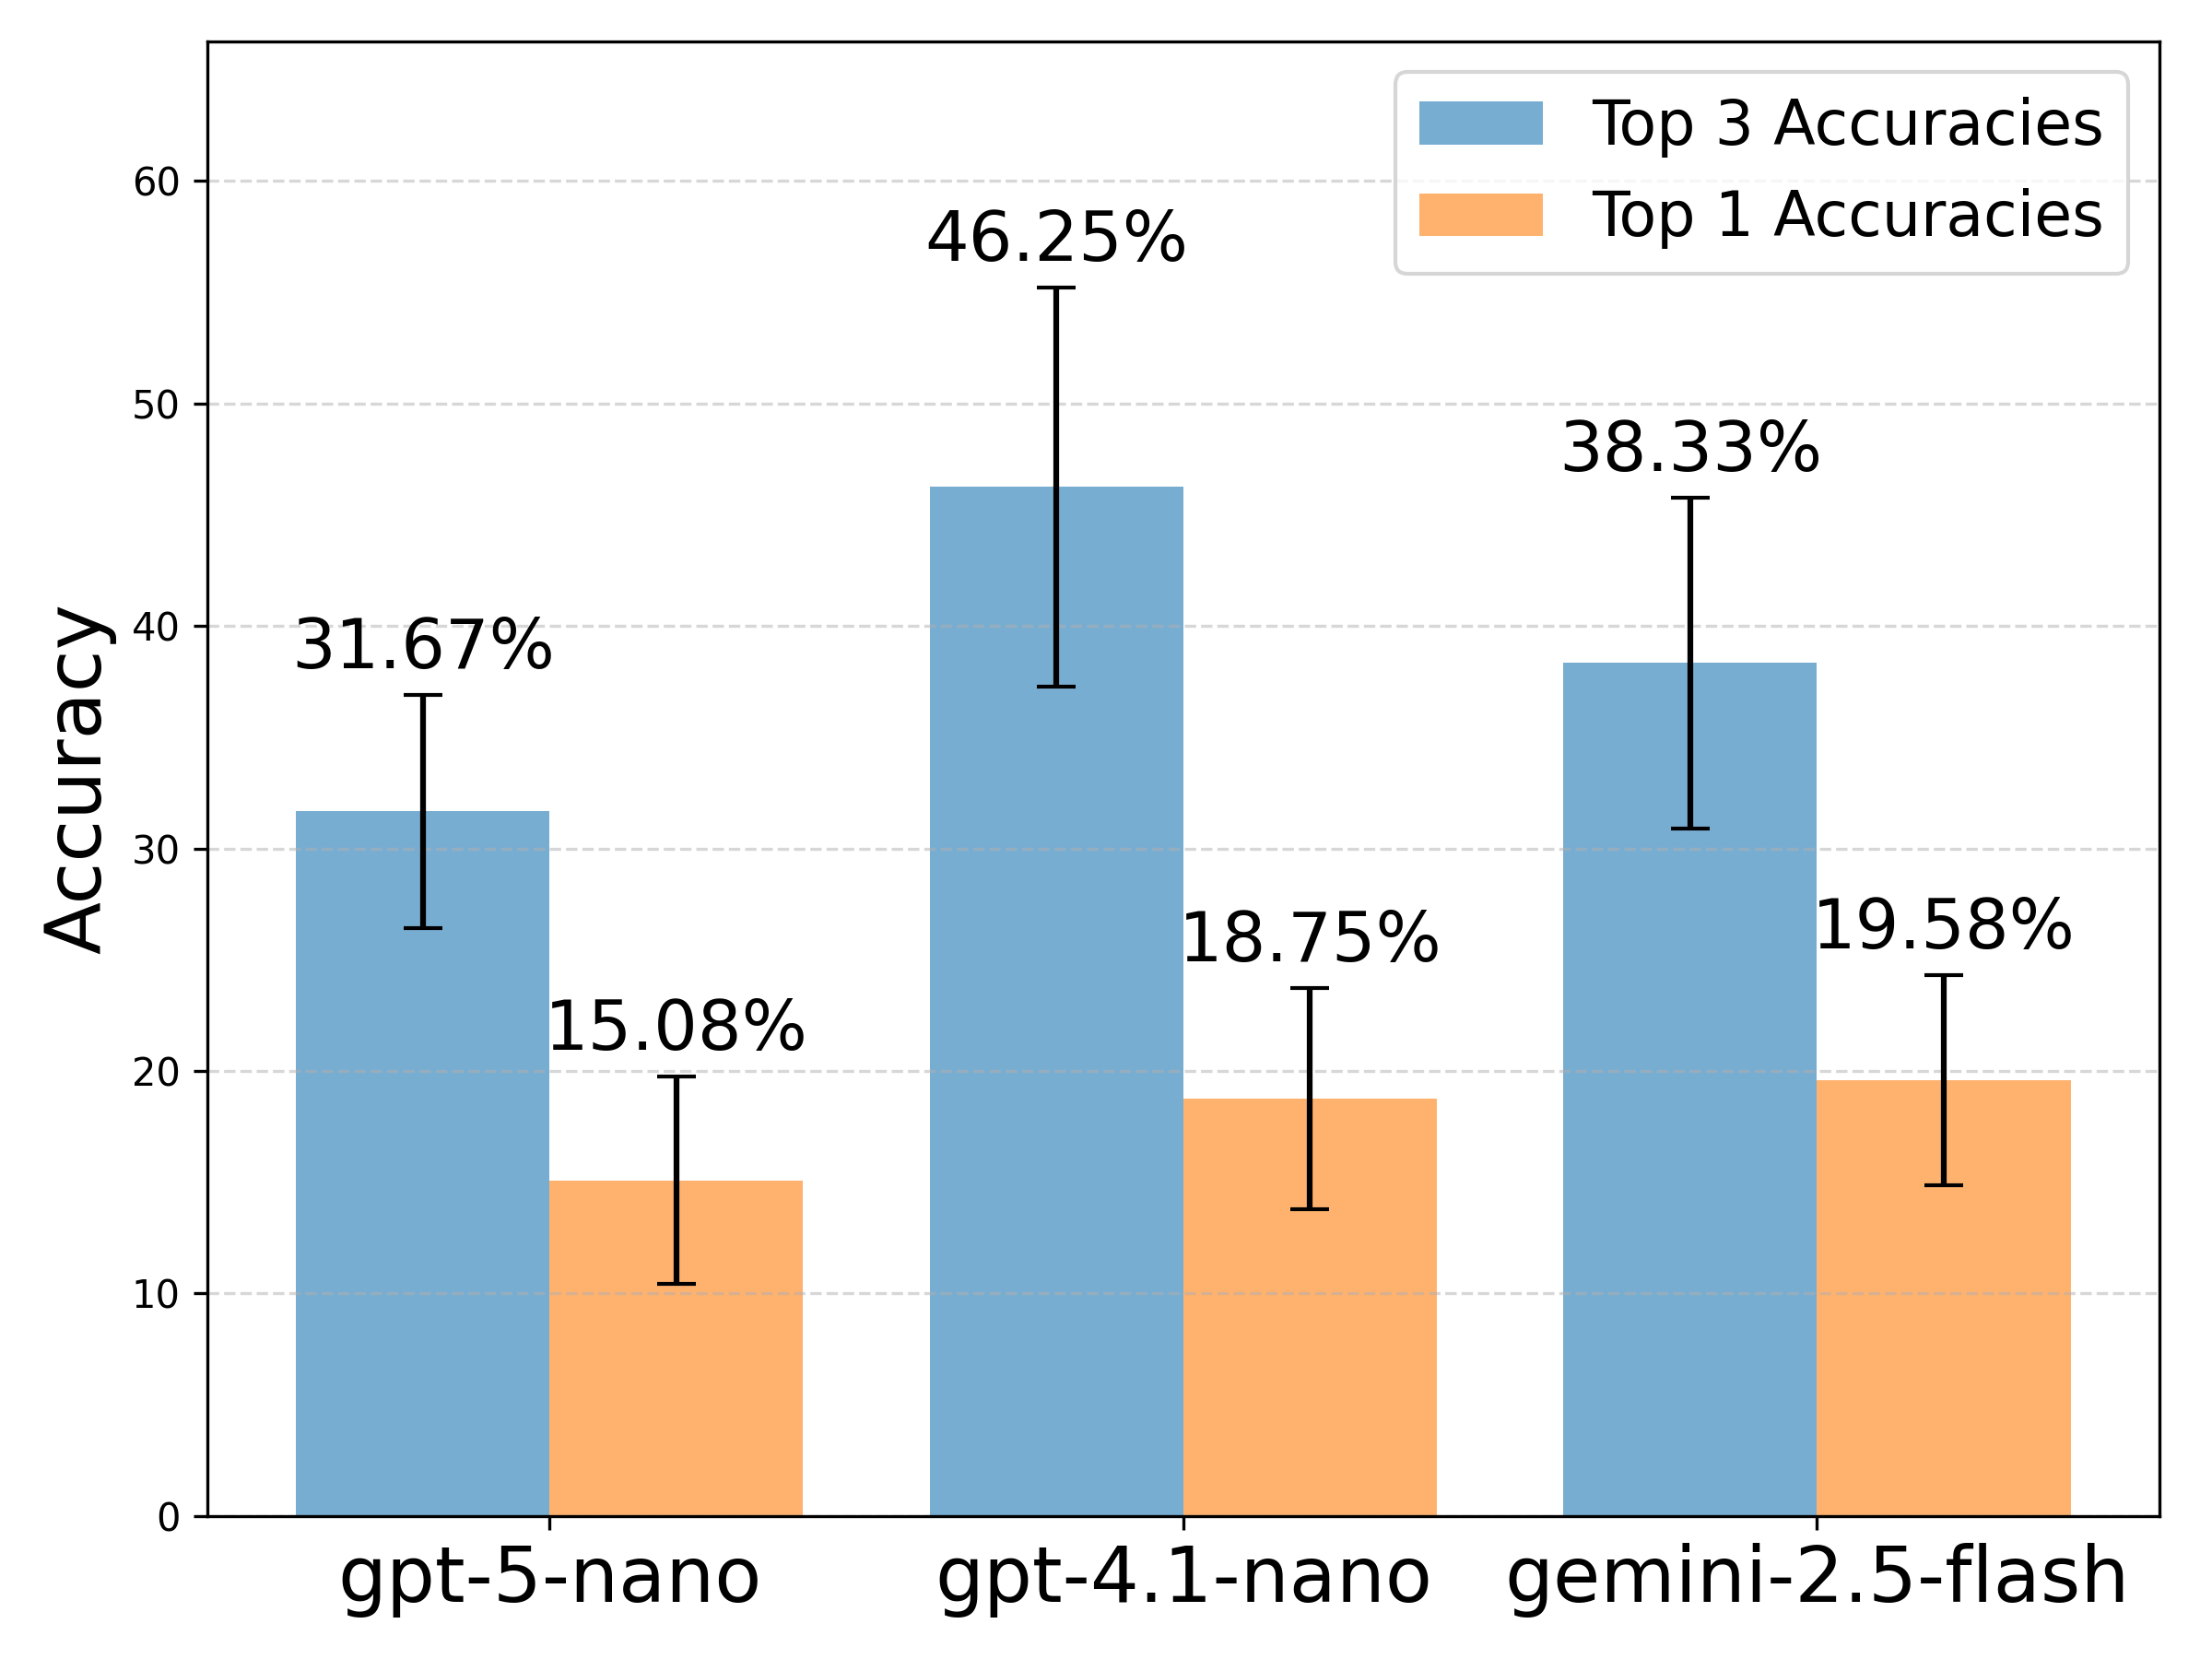
\includegraphics[width=0.9\linewidth]{figures/hotpotqa/accs_gemini-2.5-flashnew.png}
    \caption{Accuracy with gemini-2.5-flash as the Actor. Speculating multiple actions ($k=3$) yields higher accuracy than predicting a single action.}% suggesting that the number of speculative actions can be an effective hyperparameter to tune}
    \label{fig:hotpotqa_accs}
    \vspace{-10pt}
\end{wrapfigure}
We further evaluate our framework on HotpotQA, a setting where the main performance bottleneck arises from information retrieval latency. In this example, the agent must answer multi-hop questions through sequential Wikipedia API calls~\citep{yang2018hotpotqadatasetdiverseexplainable}, mirroring real-world agentic workflows with high round-trip network latency. In this setting, the Speculator predicts likely Wikipedia content while the actual API call executes. Parallelism allows the agent to continue reasoning on provisional information rather than blocking on API latency. % We leave the details of the experimental setup to
See Appendix~\ref{app:hotpotqa} for details about our experimental setup.

We evaluate on the accuracy of the predicted API calls. As shown in Figure \ref{fig:hotpotqa_accs}, the Speculator successfully predicts ground truth API call up to $46\%$ of the time with top-3 prediction. This accuracy improves significantly from top-1 to top-3 predictions, yielding substantial accuracy gains with modest speculation width increase. Our speculation provides value by precomputing reasoning paths during otherwise idle API waiting time. 

\section{Beyond Lossless Speculation: OS Hyperparameter Tuning Environment}
\label{sec:os-speculation}
Thus far, our experiments have focused on \emph{lossless} speculation, where speculative actions are validated sequentially before commitment. We now turn to a \emph{lossy} setting that relaxes this constraint.
In latency-sensitive environments like an operating system, 
waiting for a powerful but slow Actor (10-15s deliberation) can leave the system in a degraded state.
Instead, we use a fast Speculator to apply immediate provisional adjustments while the Actor deliberates. 
This is made safe by a last-write-wins mechanism—the Actor's final decision 
simply overwrites any speculative action, 
removing the need for complex rollbacks. 
This method accelerates convergence and improves reaction time, 
which we evaluate on the \texttt{sysbench cpu} benchmark, a CPU-bound workload~\citep{sysbench}.
%Our framework extends the work of~\cite{liargkovas2025llmTuning}, by introducing a fast, speculative loop to mitigate the deliberation latency of the expert Actor.
\subsection{Experimental Setup}
We tune Linux's Completely Fair Scheduler (CFS) parameter \texttt{min\_granularity}, 
which controls a task's minimum timeslice. 
This knob strongly affects scheduling performance: smaller timeslices reduce latency but can degrade throughput, yielding a classic trade-off. Building on~\citep{liargkovas2025llmTuning}, we augment the prior LLM-based tuning setup with a speculative control loop.
% Prior work~\citep{liargkovas2025llmTuning} demonstrated that an LLM-based agent can optimize this parameter; here, we extend that setup with a speculative control loop.
% Our system consists of a fast Speculator and a slow Actor. 

The Speculator proposes a parameter update each second using the latest performance metric. 
The Actor, in contrast, responds every 10–15 seconds after analyzing a compressed chronology of the Speculator's recent (measurement, action) pairs.
Upon arrival, the Actor’s decision is applied immediately and its state resets the Speculator’s context, preventing drift from the validated narrative.

\vspace{-5pt}
\paragraph{Evaluation}
%\vspace{-5pt}
We evaluate three systems: (1) \textbf{Actor-only}: slow but deliberative (10-15\,s interval); (2) \textbf{Speculator-only}: fast (1\,s interval) but non-extensive; (3) \textbf{Speculator–Actor}: combined system using speculative updates between Actor decisions.
% We are interested in (i) reaction time, (ii) convergence speed to the optimal setting, and (iii) ability to avoid local minima that trap the Speculator-only baseline.


\subsection{Results}
\begin{figure*}[t]
 \centering % Center the entire figure content
 % --- Left Column: The Plot ---
 \begin{minipage}[c]{0.64\linewidth}
  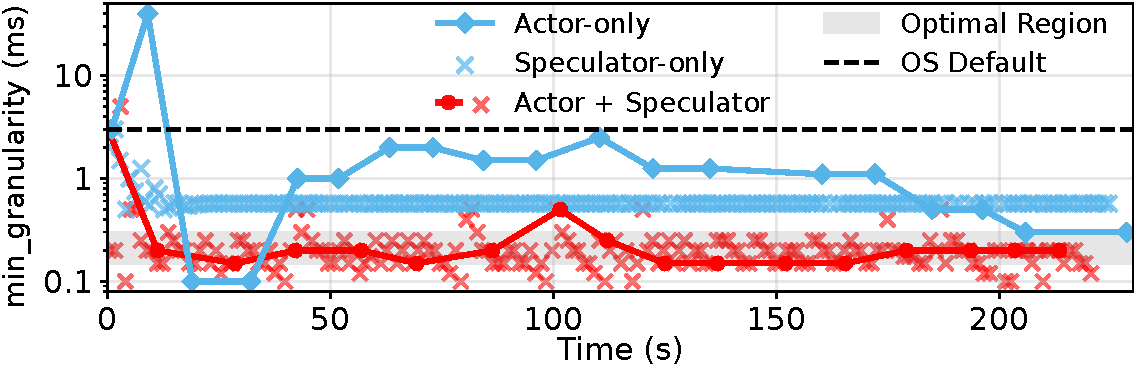
\includegraphics[width=\linewidth]{figures/os_tuning/combined_plot.pdf}
 \end{minipage}
 \hfill % Adds a flexible space between the two columns
 % --- Right Column: The Table ---
 \begin{minipage}[c]{0.35\linewidth}
  \centering
\begin{tabular}{l p{1.29cm}}
  \toprule
  \textbf{Configuration} & \textbf{Latency p95 (ms)} \\
  \midrule
  Untuned & 102.97\\
  Actor-only      &  54.00 \\
  Actor + Spec.   &  37.93 \\
  \bottomrule
\end{tabular}
 \end{minipage}
 \caption{
 \textbf{(Left)} Comparison of \textbf{Speculator-Actor}, \textbf{Speculator-only}, and \textbf{Actor-only} convergence.
 The Speculator shortens time spent exploring poor settings. 
 The Speculator-only agent stabilizes quickly but at a worse final value.
 \textbf{(Right)} Average p95 latency over a 20-second tuning experiment showing that rapid reaction offers immediate performance benefits (see \S\ref{app:speculative-mitigation}). Lower is better.}
 \label{fig:os-speculation}
 \vspace{-10pt}
\end{figure*}

% \paragraph{Speculator mitigates poor-reaction slowdowns} The Speculator dramatically improves reaction time, as observed Figure \ref{fig:os-speculation}~(Right). During the recovery period, the full Speculator-Actor system maintains an average p95 latency of 37.93 ms. This is a substantial improvement over the Actor-only baseline, which was forced to endure the poor performance for much longer and averaged 54.00 ms. The Speculator's rapid correction prevents the system from lingering in a high-latency state (initially 102.97 ms), providing immediate benefits while the slower Actor deliberates (the full experiment is detailed in \S\ref{app:speculative-mitigation}).
% \vspace{-5pt}
% \paragraph{Speculator accelerates convergence to optimum}
% The Speculator's high-frequency updates also significantly accelerate convergence. 
% As shown in Figure~\ref{fig:os-speculation} (Left), the Speculator-Actor system reaches an optimal setting (e.g., 0.2\,ms \texttt{min\_granularity}) in approximately 10–15 seconds. 
% In contrast, the Actor-only agent takes around 200 seconds---20x slower---and remains trapped in highly suboptimal states (e.g., latency $>$120\,ms) for a long period of time. 
% The Speculator's rapid exploration provides the Actor with a richer performance landscape, allowing it to steer the system away from these pathological regions more quickly.

% \vspace{-5pt}
% \paragraph{Speculator-only is good, but not optimal}
% Figure~\ref{fig:os-speculation} also shows that while the Speculator-only system reacts quickly, it converges prematurely to a suboptimal configuration: \texttt{min\_granularity} of 0.55\,ms (36.24\,ms latency). 
% This is significantly worse than the 0.2\,ms (30.26\,ms latency) achieved by the full Speculator-Actor system. Without the Actor's guidance, the Speculator lacks the reasoning depth to escape this local minimum.
% \vspace{-5pt}
% \paragraph{Cost and latency can both decrease.}
% Because the Speculator acts as a fast explorer that accelerates convergence, the \emph{total} cost can in fact be \emph{lower}, despite launching additional speculative branches. 
% % By reaching a correct trajectory much earlier, the system avoids the prolonged high-latency exploration incurred by the Actor-only baseline.
% As shown in Table~\ref{tab:os}, the Actor-only baseline converges at roughly $200\text{s}$ with a total cost of $2.18$ cents, whereas the Actor+Speculator method converges around $13\text{s}$ with a total cost of only $0.17$ cents.

% The joint Speculator–Actor system combines fast adaptation with strategic guidance, achieving both responsiveness and optimal steady-state performance.


% \vspace{-5pt}
\paragraph{Speculator mitigates poor-reaction slowdowns.}
As shown in Figure~\ref{fig:os-speculation} (right), the Speculator significantly improves reaction time. 
During recovery, the full Speculator–Actor system maintains an average p95 latency of 37.93\,ms, compared to 54.00\,ms for Actor-only, which remains longer in degraded states (initially 102.97\,ms). 
Fast speculative updates provide immediate mitigation while the Actor deliberates (details in \S\ref{app:speculative-mitigation}).

\vspace{-5pt}
\paragraph{Speculator accelerates convergence to optimum.}
Figure~\ref{fig:os-speculation} (left) shows that the joint system reaches the optimal setting (0.2\,ms \texttt{min\_granularity}) in 10-15\,s, whereas Actor-only requires $\sim$200\,s and remains trapped in highly suboptimal regions (e.g., latency $>120$ms) for extended periods. 
Rapid speculative exploration helps the Actor avoid pathological configurations.

\paragraph{Speculator-only reacts quickly but is suboptimal.}
While Speculator-only stabilizes rapidly, it converges to a worse configuration (0.55\,ms; 36.24\,ms latency) than the joint system (0.2\,ms; 30.26\,ms). 
Without the Actor’s deeper reasoning, it cannot escape local minima.

\paragraph{Cost and latency both decrease.}
Despite additional speculative calls, total cost is lower due to faster convergence. 
As shown in Table~\ref{tab:os}, Actor-only converges at $\sim$200\,s with a total cost of 2.18\,cents, whereas Speculator–Actor converges in $\sim$13\,s with only 0.17\,cents.

Overall, the joint system combines fast adaptation with strategic guidance, achieving both responsiveness and optimal steady-state performance.
\section{Cost--Latency Tradeoff}
\label{sec:cost-latency}
Performing more speculative API calls improves accuracy but also raises costs when pricing is based on the number of calls or tokens. In this section, assume a fixed token per unit time and fixed per token cost, and analyze the cost-latency tradeoff. Full details can be found in Appendix~\ref{app:cost-latency}.

\subsection{Static breadth-focused Speculation 
(Algorithm~\ref{alg:speculative-k})}
\label{subsec:breadth}
In addition to Proposition~\ref{thm:improvement}, we obtain a closed-form expression for relative cost increase ratio. Thus a user can tune the number of speculative branches to launch ($k$) offline based on these expressions.
\begin{theorem}[Cost of Breadth Speculation]
\label{thm:cost-latency-tradeoff}
Under the same setting as Proposition~\ref{thm:improvement}. Let
$
(M_{\mathrm{spec}}, \E[M_{\mathrm{spec}}])
$
denote the sequential token cost and the expected token cost under Algorithm~1. Let $\tilde{k}$ denote the number of \emph{distinct} actions produced across the $k$ speculative branches, we have
% \begin{align*}
%     \frac{\E[M_{\mathrm{spec}} - M_{\mathrm{seq}}]}{\E[M_{\mathrm{seq}}]}
%     &\xrightarrow{T\to\infty}
%     \tilde{k}
%     -
%     \left(\tilde{k}+\frac{\alpha}{\alpha+\beta}\right)
%     \frac{p(k)}{1+p(k)}.
% \end{align*}
\begin{align*}
    \frac{\E[M_{\mathrm{spec}} - M_{\mathrm{seq}}]}{\E[M_{\mathrm{seq}}]}
    &=\tilde{k}
    -\frac{1}{T}\left(\tilde{k}+\frac{\alpha}{\alpha+\beta}\right)
    \left[
        \frac{(T-1)p(k)}{1+p(k)}
        +\frac{p(k)^2}{(1+p(k))^2}
        -\frac{p(k)^2}{(1+p(k))^2}(-p(k))^{T-1}
    \right]
    \\
    &\xrightarrow{T\to\infty}
    \tilde{k}
    -
    \left(\tilde{k}+\frac{\alpha}{\alpha+\beta}\right)
    \frac{p(k)}{1+p(k)}.
\end{align*}
Note that $\tilde{k}$ is possibly different from $k$ because the $k$ independent speculations might have duplications, in which case we kill the duplicated speculation processes.
% \begin{align*}
%     \frac{E[T_{\mathrm{seq}} - T_{\mathrm{spec}}]}{E[T_{\mathrm{seq}}]}
%     \xrightarrow{\;\;T\to\infty\;\;}
%     \frac{p(k)}{1+p(k)}\cdot\frac{b}{a+b}
% \qquad
%     \frac{\E[M_{\mathrm{spec}} - M_{\mathrm{seq}}]}{\E[M_{\mathrm{seq}}]}
%     \xrightarrow{T\to\infty}
%     \frac{k}{1+p(k)}-\frac{b}{a+b}
%     \frac{p(k)}{1+p(k)}
% \end{align*}
% where $p(k) = 1-(1-p)^k$ is the success probability of at least one of the $k$ speculations.
\end{theorem}
Proof of the above theorem is given in Appendix~\ref{app:cost-latency}. Comparing Proposition~\ref{thm:improvement} with Proposition~\ref{thm:cost-latency-tradeoff}, we see that both ratios are governed by $p(k)$. Therefore, given an estimation of $p(k)$, a user can directly use these expressions to tune $k$ as a knob, trading off cost increase against latency decrease offline. Interestingly, our experiment (Figure~\ref{fig:threshold}) exactly shows this non-linear dependence on $k$ in the cost increase ratio, as the $p(k)$ increases when $k$ increases.


% \subsection{Breadth-focused Speculation 
% (Algorithm~\ref{alg:speculative-k})}
% \label{subsec:breadth}
% In addition to Proposition~\ref{thm:improvement}, we obtain a closed-form expression for relative cost increase ratio
% \begin{align*}
% \lim_{T\to\infty}\frac{\E[M_{\mathrm{spec}} - M_{\mathrm{seq}}]}{\E[M_{\mathrm{seq}}]}
%     \leq k-\left(k+\frac{\alpha}{\alpha+\beta}\right)
%     \frac{p(k)}{1+p(k)}.
% \end{align*}
% See Theorem~\ref{thm:cost-latency-tradeoff} in Appendix~\ref{app:cost-latency} for the formal theorem. Comparing Proposition~\ref{thm:improvement} with the above expression, we see that both ratios are governed by $p(k)$. Thus, given an estimation of $p(k)$, a user can directly tune $k$ offline, trading off cost against latency. Our experiment (Figure~\ref{fig:threshold}) shows this non-linear dependence on $k$, and additional empirical results can be found in Appendix~\ref{app:additional-empiricals}.
\subsection{Dynamic selective speculation} 
\label{subsec:dynamic-speculation}
\begin{wrapfigure}{r}{0.465\columnwidth}
\vspace{-10pt}
    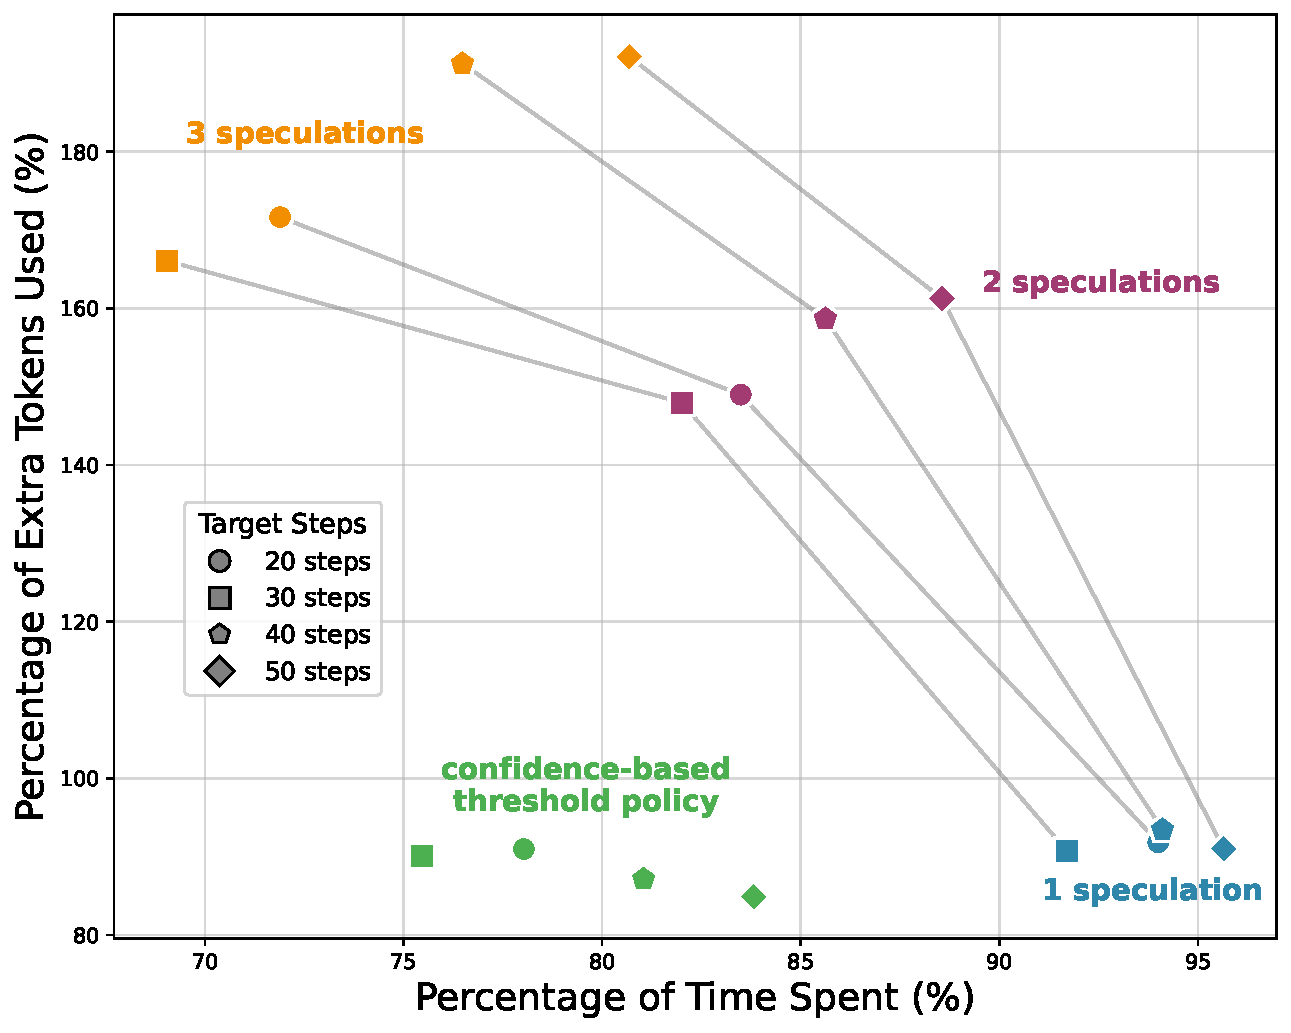
\includegraphics[width = 0.95\linewidth]{figures/chess/plot_with_confidence.pdf}
    \caption{Cost-latency tradeoff across different speculation widths, forming a Pareto curve.
    The confidence-based heuristic attains the lowest cost at latency comparable to three fixed predictions, outperforming fixed one- or two-branch strategies.
    }
    \vspace{-20pt}
    \label{fig:threshold}
\end{wrapfigure}
So far we assume a fixed branch accuracy $p$. In practice, we sometimes are able to obtain per-speculation confidence estimates (e.g., from intrinsic model logits, or from a separately-trained auxiliary predictor), allowing confidence-aware selective speculation. At each speculation window,
the accuracies of the $k$ speculative branches are random and drawn from a known distribution (which may vary over time). Before acting, the realized accuracy vector $\mathbf p = (p^1,\dots,p^k)$ is observed, and we choose how many of the top branches to launch.

We model the cost-latency tradeoff via the weighted objective
\begin{equation*}
    \max \; r\cdot\sum_{t=1}^T\mathrm{latency} - c\cdot\sum_{t=1}^T\mathrm{cost}
\end{equation*}
where $r$ and $c$ encode the relative importance of latency and cost. For simplicity, let $a$ and $b$ denote the fixed latency of the actor and speculator, and define the latency gain $\ell = r(a-b) > 0$.

% We again assume a fixed horizon $T$ and $k$-branch speculation. Suppose that at each time step, there is a known joint distribution $F_t$ from which the actual accuracy vector $\mathbf P_t = (P_t^1,\dots,P_t^k) \in [0,1]^k$ of each speculative branch is drawn from. Note that the distributions $F_t$ can vary across time step. At time step $t$, if currently there is a speculation window, i.e., the previous step did not result in a hit and thus this step is a cached action, then we observe an instantiated accuracy vector $\mathbf P_t = (P_t^1,\dots,P_t^k) \in [0,1]^k$. Based on these observed accuracies, our goal is to select a subset of these branches to accept. 

If the top $m$ branches are launched, the probability of a cached step is
$
q(m;\mathbf p)
=
1 - \prod_{j=1}^{m}(1-p^{(j)}),
$
where $p^{(1)} \ge \dots \ge p^{(k)}$ are the sorted confidences.

% \begin{theorem}[Finite-horizon two-mode dynamic program]
% \label{thm:dynamic-general}
% There exist scalars $\Delta_t$ (computed by backward recursion)
% such that at each speculation window $t$, after observing $\mathbf p$,
% the optimal number of branches satisfies
% \[
% m_t^\star(\mathbf p)
% \in
% \arg\max_{m \in \{0,\dots,k\}}
% \{ q(m;\mathbf p)\,\Delta_t - c m \},
% \]
% The continuation value $\Delta_t$ satisfies
% \[
% \Delta_T = 0, 
% \qquad
% \Delta_t
% =
% \ell
% -
% \mathbb E
% \Big[
% \max_m \{ q(m;\mathbf P)\,\Delta_{t+1} - c m \}
% \Big]\quad t=T-1, \dots, 1
% \]
% \end{theorem}
% The key implication is structural: \emph{dynamic selective speculation reduces to a one-dimensional trade-off}. 
% At each window, additional branches are launched only if their incremental hit probably, scaled by the continuation value $\Delta_t$, exceeds the per-branch cost $c$. All intertemporal effects are summarized by the single scalar $\Delta_t$.

% Furthermore, under stationary (the distribution of the accuracies is homogeneous) average-reward approximation, the structure simplifies further.

% \begin{corollary}[Stationary threshold rule (informal)]
% \label{cor:stationary-approximation}
% There exists a constant
% $\Delta^\star$ such that at any speculation window,
% the optimal breadth satisfies
% $m^\star(\mathbf p)
% \in
% \arg\max_{m}
% \{ q(m;\mathbf p)\,\Delta^\star - c m \}$. Equivalently, branches are added greedily in descending confidence order
% while $\Delta^\star \cdot \delta q(m;\mathbf p) \ge c$, with $\delta$ denoting the marginal gain from adding one more branch.
% \end{corollary}
% \paragraph{Practical takeaway.}
% The policy reduces to estimating a single scalar $\Delta^\star$ offline
% (e.g., from the stationary average-reward analysis).
% At runtime, given the confidences, the system sorts them
% and incrementally adds branches while the marginal gain in hit probability,
% scaled by $\Delta^\star$, exceeds the per-branch cost $c$.
% This requires only $O(k)$ computation per step and avoids solving a
% dynamic program online.
\vspace{10pt}
\begin{theorem}[Confidence-aware selective speculation]
\label{thm:dynamic-general}
There exist scalars $\Delta_t$ such that at each speculation window $t$, the optimal breadth satisfies
\[
m_t^\star(\mathbf p)
\in
\arg\max_{m \in \{0,\dots,k\}}
\{ q(m;\mathbf p)\,\Delta_t - c m \}.
\]
The continuation values are given by the backward recursion
\[
\Delta_T = 0, \qquad
\Delta_{1::T-1}
=
\ell
-
\mathbb E
\Big[
\max_m \{ q(m;\mathbf P)\,\Delta_{t+1} - c m \}
\Big]
\]
In the stationary case (time-homogeneous accuracy distribution), the continuation values 
$\Delta_t$ collapse to a single constant $\Delta^\star$. Thus branches are added greedily in descending confidence order
while
$\Delta^\star \cdot \delta q(m;\mathbf p) \ge c$, 
where $\delta q(m;\mathbf p)$ is the marginal gain from adding one more branch.
\label{thm:dynamic}
\end{theorem}
\paragraph{Interpretation and implementation}
The key implication is structural: dynamic selection collapses to a one-dimensional trade-off. 
Additional branches are launched only when their incremental hit probability,
scaled by a single continuation value ($\Delta_t$ or $\Delta^\star$),
exceeds the marginal cost $c$.
Under stationarity, this reduces to estimating $\Delta^\star$ offline;
at runtime, the system simply sorts confidences and adds branches greedily,
requiring $O(k)$ computation per step.

\paragraph{Empirical results} We implement a simple constant-threshold approximation of the stationary rule in the chess environment. At each step, after generating speculative branches, we use a predictor to estimate the correctness probability of each branch and continue only with those whose predicted accuracy exceeds 50\%. This implements a simplified threshold rule consistent with the structure suggested by Theorem~\ref{thm:dynamic}. Our method achieves the \emph{lowest additional token cost} while providing \emph{greater latency reduction} than naively launching 1 or 2 speculations per step.
\subsection{Depth-focused speculation} 
\label{subsec:depth-focused}
The previous two strategies are breadth-focused: each speculation is immediately followed by a real API call (speculative depth 1). Additionally, we analyze the opposite extreme: a \emph{depth-focused} policy, in which multi-step speculations are continuously spawned. Somewhat counterintuitively, this strategy does \emph{not} lead to exponential branch growth. Speculative calls are only extended when either a speculative or real call returns, and inconsistent subtrees are immediately pruned. Consequently, the system can run at most $a/b$ speculative steps ahead (governed by the relative speeds of real vs. speculative calls), ensuring that the number of active branches remains bounded and \emph{does not scale with the horizon $T$}. Under this policy, we can show that (formal theorem in Appendix~\ref{thm:depth})
\[
    \frac{\E[T_{\mathrm{seq}} - T_{\mathrm{spec}}]}{\E[T_{\mathrm{seq}}]}
    = \frac{T-1}{T} \, p \Bigl(1 - \frac{b}{a}\Bigr),\qquad
    \frac{\E[M_{\mathrm{spec}} - M_{\mathrm{seq}}]}{\E[M_{\mathrm{seq}}]}
    \approx\frac{T-1}{T}\left((1-p)\left(\frac{a}{2b}-\frac{1}{2}\right)+p\right)
\]
Compared to breadth speculation, depth speculation improves the latency coefficient from $\frac{p}{1+p}$ to $p$, increasing the theoretical speedup ceiling from $\frac{1}{2}$ to $1$. 
The cost term scales with $(1-p)(\frac{a}{2b}-\frac{1}{2})$, which captures how many speculative steps can accumulate before the real response arrives. 

% \subsection{Depth-focused speculation.} 
% \label{subsec:depth-focused}
% The previous two strategies are breadth-focused: each speculation is immediately followed by a real API call (speculative depth 1). Additionally, we analyze the opposite extreme: a \emph{depth-focused} policy, in which multi-step speculations are continuously spawned. Somewhat counterintuitively, this strategy does \emph{not} lead to a unbounded exponential blowup in the number of parallel branches. Speculative calls are only extended when either a speculative or real Actor call returns, and any subtree inconsistent with the real outcome is immediately pruned. Consequently, the system can run at most $a/b$ speculative steps ahead (governed by the relative speeds of real vs. speculative calls), ensuring that the number of active branches remains bounded and \emph{does not scale with the horizon $T$}.
% \begin{theorem}[Cost--Latency Tradeoff for Depth Speculation]
% Let $p$ be the baseline correctness probability of a speculative guess. Let $a$ and $b$ denote the fixed latency of real API and each speculation for simplicity. Using the same $T$ and $M$ notation, we have
% \[
%     \frac{\E[T_{\mathrm{seq}} - T_{\mathrm{spec}}]}{\E[T_{\mathrm{seq}}]}
%     = \frac{T-1}{T} \, p \Bigl(1 - \frac{b}{a}\Bigr),\qquad
%     \frac{\E[M_{\mathrm{spec}} - M_{\mathrm{seq}}]}{\E[M_{\mathrm{seq}}]}
%     \approx\frac{T-1}{T}\left((1-p)\left(\frac{a}{2b}+\frac{1}{2}\right)+p\frac{b}{a}\right)
% \]
% \end{theorem}


% This result highlights two contrasts with breadth speculation.
% First, the latency-speedup coefficient improves from $\frac{p}{1+p}$ (breadth) to $p$ (depth), raising the theoretical upper limit from $\tfrac{1}{2}$ to $1$. Second, the key term in the cost ratio, $(1-p)(\tfrac{a}{2b}+\tfrac{1}{2})$, reflects how many speculative steps can be launched before the real Actor response arrives. In the limit of perfect speculative accuracy, the ratio simplifies to $b/a$, corresponding to the extra cost of attaching a single speculative call to each real action.

\section{Conclusion}
\label{sec:conclusion}
In this paper we propose \textbf{Speculative Actions}, a lossless framework for accelerating general agentic environments by breaking the strict sequentiality of their interaction loops. Our approach treats every step, whether an LLM call, tool invocation, MCP request, or human response, as an API call subject to prediction and parallelization. By pairing a fast \emph{Speculator} with a slow but authoritative \emph{Actor}, the framework enables agents to anticipate and prepare likely next actions in parallel, transforming otherwise idle waiting time into productive computation. We instantiate the framework across four representative environments and observe consistent substantial latency reduction. Finally, we provide a cost-latency analysis that addresses the tradeoff between the additional cost and the latency gains from launching additional speculative actions.
% Notably, while most environments adopt a strictly lossless validation process, our OS hyperparameter experiment demonstrates that relaxing this constraint enables fast exploratory updates, extending speculation to adaptive control scenarios.

% More broadly, speculative actions reveal a systems-level design principle for modern agents: \emph{ parallelism in environment interactions}. Future work could extend this idea through multi-step and uncertainty-aware speculation, tighter integration with reinforcement learning and environment simulators. Together, these directions point toward general-purpose, real-time agentic systems where speculation becomes a first-class mechanism for efficient decision making.







% \section*{Ethics Statement}
% We confirm that all authors have read and adhered to the ICLR Code of Ethics. Our work introduces a framework for accelerating AI agents, which has several ethical dimensions. The "lossy" OS tuning agent directly modifies a live system's parameters, which carries inherent risks if not properly managed. We address this by proposing safety mechanisms such as last-write-wins for easy rollbacks and discussing the importance of safety envelopes and repair paths, as detailed in our framework (\S\ref{framework}) and the OS tuning case study (\S\ref{sec:os-speculation}). While our e-commerce and human-expert experiments were conducted using simulators and consenting expert participants, the deployment of such agents in real-world human-in-the-loop systems would require further study into user experience and safety. The underlying LLMs may also inherit biases from their training data, and care must be taken to evaluate and mitigate these before deployment in sensitive, user-facing applications.

% \section*{Reproducibility Statement}
% We are committed to ensuring the reproducibility of our work. To this end, all source code for our speculative action framework, experimental environments, and analysis scripts will be made publicly available . Our experiments are conducted on publicly available benchmarks, including TextArena for chess, $\tau$-bench for e-commerce, and HotpotQA for web search, ensuring that other researchers can build upon our results. The OS tuning experiments use the open-source sysbench tool.

% Details regarding the experimental setup, including hardware specifications, software versions, and specific configurations for each environment, are provided in the main text and extensively in \S\ref{app:additional_details}. This includes the specific LLMs used (e.g., GPT and Gemini model families), reasoning budgets, and the exact prompts. The core logic of our framework is detailed in Algorithm~\ref{alg:speculative-k}. We believe these resources provide a clear path for reproducing our findings.


%\input{sections/discussion}
% \subsubsection*{Author Contributions}
% If you'd like to, you may include  a section for author contributions as is done
% in many journals. This is optional and at the discretion of the authors.

% \subsubsection*{Acknowledgments}
% Use unnumbered third level headings for the acknowledgments. All
% acknowledgments, including those to funding agencies, go at the end of the paper.

\subsubsection*{Acknowledgments}
This work was partially supported by the Columbia-Dream Sports AI Innovation Center.

\bibliography{iclr2026_conference}
\bibliographystyle{iclr2026_conference}

\appendix
\newpage
\section{Proof of Proposition \ref{thm:improvement}}
\label{app:proof}
\begin{proof}
\textbf{Baseline.}  
In sequential execution, each of the $T$ steps requires one call to the true model $h$ with mean latency $1/\beta$. Therefore
\[
E[T_{\mathrm{seq}}] \;=\; \frac{T}{\beta}.
\]

\medskip
\textbf{Expected time saved per hit.}  
Consider two consecutive steps $(t,t{+}1)$. In the baseline, the total completion time is $R = B + C$, where $B,C \sim \mathrm{Exp}(\beta)$ are the latencies of step $t$ and step $t{+}1$. With speculation, we launch $A \sim \mathrm{Exp}(\alpha)$ during step $t$. If the guess is correct, the $(t{+}1)$ call $C$ can be issued once either $A$ or $B$ finishes, so the block completes at
\[
S \;=\; C + \min\{A,B\}.
\]

Thus, when a guess is correct, our expected time saved is
\[
R - S \;=\; (B-A)_+,
\]
where $(x)_+ = \max\{x,0\}$.
  
By independence of $A,B$,
\[
\mathbb{E}[(B-A)_+]
= \int_{0}^{\infty}\!\int_{0}^{b} (b-a)\,\alpha e^{-\alpha a}\,\beta e^{-\beta b}\,da\,db
= \frac{\alpha}{\beta(\alpha+\beta)}.
\]

\medskip
\textbf{Expected number of hits}. We denote the expected number of hits by round $n$ as $S_n$, that is
$$\E[\text{number of hits by round }n] = S_n$$
We then have $S_0=0$, $S_1 = p(k)$. In round $1$, either (i) we hit with probability $p(k)$, in which case round $2$ cannot be a hit (there is no speculation window immediately after a correct speculation), contributing $1+S_{n-2}$; or (ii) we miss with probability $1-p(k)$, after which round $2$ proceeds normally, contributing $S_{n-1}$. We then have the following recursion
$$S_n = p(k)(1+S_{n-2}) + (1-p(k))S_{n-1}$$
Solve this linear recurrence by splitting into homogeneous and particular parts.

\textit{(1) Homogeneous part}
\[S_n^{h} = p(k)S_{n-2}+ (1-p(k))S_{n-1}\]
The characteristic equation is
\[
r^2-(1-p(k))r-p(k)=0=(r-1)(r+p(k)) \implies \text{the roots are }r_1=1, r_2=-p(k)
\]
Therefore,
\[
S_n^{(h)}=C_1 + C_2(-p(k))^n.
\]

\textit{(2) Particular solution}
The forcing term is constant ($+p(k)$), and $r=1$ is a root, so a constant trial collides with the homogeneous part. Try $S_n^{(p(k))}=an$ and substitute:
\[
an=(1-p(k))a(n-1)+p(k)a(n-2)+p(k)
= an - a(1+p(k)) + p(k),
\]
which gives $a(1+p(k))=p(k)$ and thus
\[
S_n^{(p(k))}=\frac{p(k)}{1+p(k)}\,n.
\]

Combine:
\[
S_n = C_1 + C_2(-p(k))^n + \frac{p(k)}{1+p(k)}\,n.
\]
Use $S_0=0$ and $S_1=p(k)$:
\[
0=C_1+C_2,\qquad
p(k)=C_1 + C_2(-p(k)) + \frac{p(k)}{1+p(k)}.
\]
Solving yields $C_2=-\dfrac{p(k)^2}{(1+p(k))^2}$ and $C_1=\dfrac{p(k)^2}{(1+p(k))^2}$.

Hence the closed form solution is
\[
S_n=\frac{p(k)}{1+p(k)}\,n+\frac{p(k)^2}{(1+p(k))^2}\Bigl(1-(-p(k))^n\Bigr)
\]

\medskip
\textbf{Total saving.}  
There are $T-1$ potential speculation windows, hence
\[
E[T_{\mathrm{s}}]
= \frac{T}{\beta} - S_{T-1}\frac{\alpha}{\beta(\alpha+\beta)}
\]

\medskip
\textbf{Final ratio.}  
Dividing by $E[T_{\mathrm{seq}}] = T/\beta$ gives
\[
    \frac{E[T_{\mathrm{s}}]}{E[T_{\mathrm{seq}}]}
    \;=\;
    1 - \frac{1}{T}\frac{\alpha}{\alpha+\beta}\left[\frac{(T-1)p(k)}{1+p(k)}+\frac{p(k)^2}{(1+p(k))^2} - \frac{p(k)^2}{(1+p(k))^2}(-p(k))^{T-1}\right]
\]
\end{proof}
Taking $T\to\infty$, we get exactly that the ratio converges to $1-\frac{p(k)}{1+p(k)}\frac{\alpha}{\alpha+\beta}$



\newpage
\section{Additional Environment Details}
\label{app:additional_details}

% \subsection{Chess}
% \begin{figure}
%     \centering
% \includegraphics[width=0.6\linewidth]{figures/chess/combined_time_token_plot.pdf}
%     \caption{Percentage of extra tokens used against percentage of time saved for different numbers of predictions at different numbers of steps, averaged across $5$ runs.}
%  \label{fig:chess_time_token_plot}
% \end{figure}

% \paragraph{Trade-off between Time Saved and Token Cost.} In addition to time savings, we also measure the additional token cost of parallel speculation. We track this using the metric \textbf{extra token percentage}: $(M_{sequantial}-M_{speculative})/{M_{sequential}}$. Figure~\ref{fig:chess_time_token_plot} shows the trade-off between time saved and token cost for each number of predictions. We observe that the extra token percentage increases as the number of predictions increases, while the time saved percentage also increases, creating a clear trade-off.

\subsection{Ecommerce}
% \begin{wrapfigure}{r}{0.45\columnwidth}
%     \centering
%     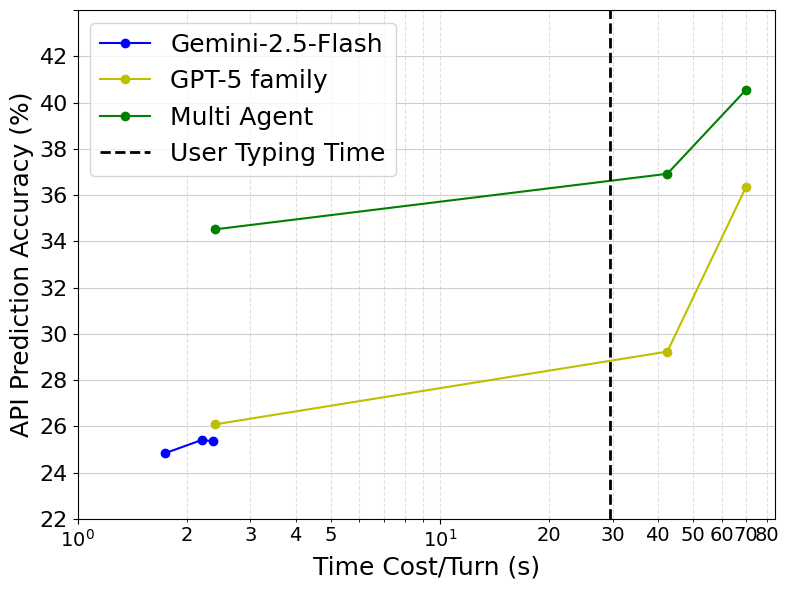
\includegraphics[width=\linewidth]{figures/ecommerce/time_accuracy.png}
%     \caption{Prediction accuracy versus speculation time. Blue and yellow curves show single-agent speculation, while the green curve shows the multi-agent setting. The dashed vertical line indicates average user typing time.}
%     \label{fig:time_accuracy}
% \end{wrapfigure}

\paragraph{$\tau$-bench:} A benchmark designed for dynamic task-oriented dialogues between a user (simulated by language models) and an API-augmented agent. The benchmark spans two domains — retail and airline, with structured databases, domain-specific tools. We focus on the retail domain, where the agent assists users with operations such as canceling or modifying pending orders, initiating returns or exchanges, or providing product and order information. The benchmark defines 115 tasks with 15 APIs (7 write, 8 read-only).




% \paragraph{Trade-off between Prediction Accuracy and Cost.}
% The time cost in Figure~\ref{fig:time_acc} consists of latency (Time to First Token) and output response time. The dashed vertical line represents the average user typing time, estimated at 40 words per minute. At this threshold, the multi-agent setting achieves approximately 34\% prediction accuracy, meaning that in over one-third of cases the agent can return an immediate response without waiting for API execution. This demonstrates that speculation can transform user experience from perceptibly laggy to effectively real-time in tool-heavy environments.

% \begin{figure}[H]
%   \centering
%   \resizebox{0.8\textwidth}{!}{%
%       \begin{subfigure}[t]{0.48\textwidth}
%         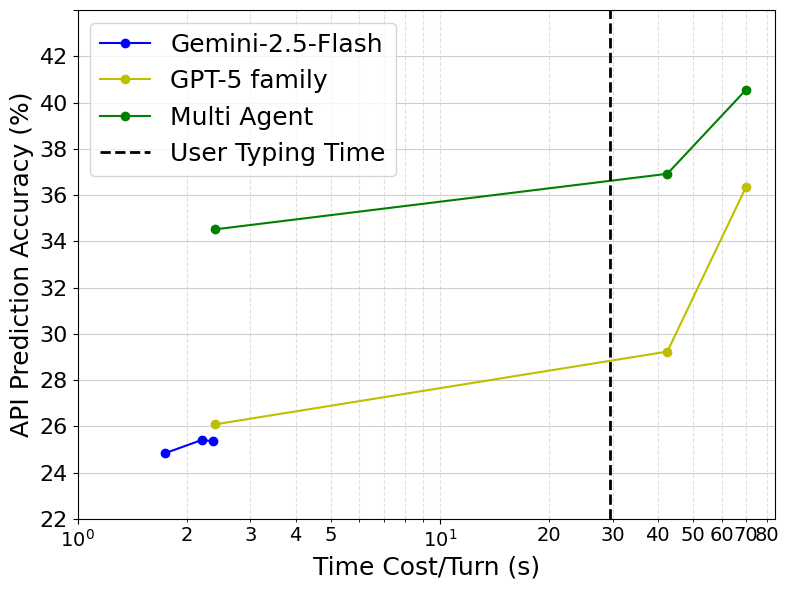
\includegraphics[width=\linewidth]{figures/ecommerce/time_accuracy.png}
%         \caption{}
%         \label{fig:time_acc}
%       \end{subfigure}
%       \hspace{0.05\textwidth} 
%       \begin{subfigure}[t]{0.48\textwidth}
%         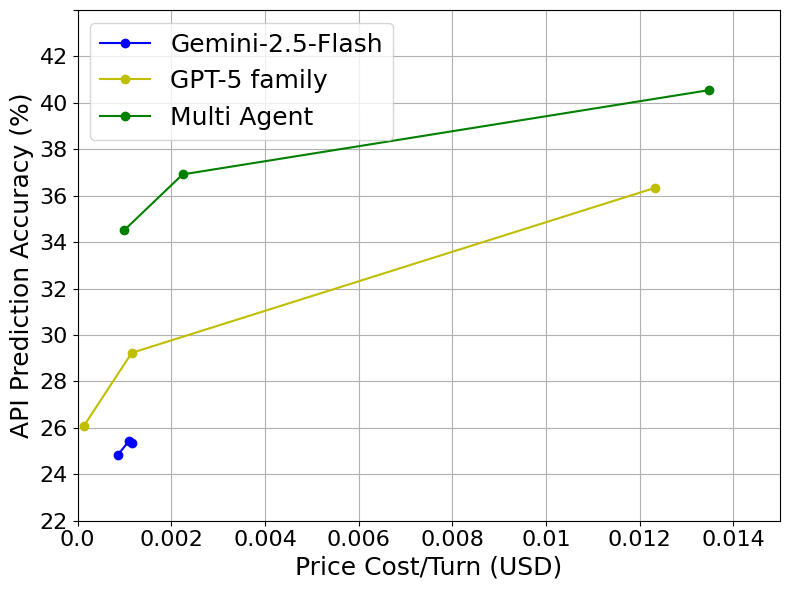
\includegraphics[width=\linewidth]{figures/ecommerce/price_accuracy.png}
%         \caption{}
%         \label{fig:price_acc}
%       \end{subfigure}
%   }
%   \caption{\textbf{Prediction Accuracy against Speculator's Cost across different models.} (a) Accuracy–Speculator time cost trade-off across models. The dashed line shows average user typing time. (d) Accuracy–Speculator price trade-off across models, reflecting the monetary cost of speculative execution.}
%   \vspace{-1em}
% \end{figure}

\subsection{HotpotQA}
\label{app:hotpotqa}
\vspace{-3pt}
% We further evaluate our framework on HotpotQA, a setting where the main performance bottleneck arises from information retrieval latency. In this example, the agent must answer multi-hop questions through sequential Wikipedia API calls \cite{yang2018hotpotqadatasetdiverseexplainable}, mirroring real-world agentic workflows with high network latency per round-trip. We apply the framework from Section~\ref{framework}, where the Speculator predicts likely Wikipedia content while the actual API call executes. This parallelism enables the agent to continue reasoning on provisional information rather than blocking on API latency.
\subsubsection{Experimental Setup}
We build our framework upon ReAct (\cite{yao2023reactsynergizingreasoningacting}), which interleaves chain-of-thought with tool use.

\textbf{Speculative Pipeline} In this scenario, the state $s_t$ consists of the entire history of reasoning traces and retrieved information (API responses). At each step, the Actor takes in the current state $s_t$,  selects an API call $h_t \in\{\text{Search(), Lookup(), Finish()}\}$ and a corresponding parameter $q_t$, e.g. Search(entity). The call $h_t(q_t)$ returns a response $a_t$, typically providing information about the queried entity. Our speculative framework operates as follows:
\begin{enumerate}[leftmargin=*]
    \item Speculator predicts the API call response $\hat{a}_t^{(i)}$, yielding predicted next states $\hat{s}_{t+1}^{(i)} = f(s_t,\hat{a}_t^{(i)})$, $i\in\{1,\dots,k\}$.
    \item Based on the states, the Actor generates reasoning traces and subsequently determines the next API decision $(\hat{h}_{t+1}^{(i)}, \hat{q}_{t+1}^{(i)})$ for $i\in\{1,\dots,k\}$.
\end{enumerate}





% defined as the entire reasoning history \[(r_i,a_i,b_i)_{1}^t \]
% where $r_i$ denotes the internal thought at step i, $a_i$ the action taken, and $b_i$ the corresponding observation that is extracted from the environment. It follows from \ref{framework} that 
% \[ b_i = h_i(q_i)\]
% where $q_i$ are the parameters of the API call $h_i$. Instead of waiting for an external environment to return the next observation $b_t$, the Speculator attempts to guess $\hat{b}_t$. 

% Formally, the speculation procedure proceeds as follows -
% \begin{enumerate}
% \item Speculate the observation $\hat{b}_t$ based on the current state $s_t$ and action $a_t$ i.e. $ \hat{b}_t = \hat{h}(s_t, a_t)$
% \item The agent simulates the next thought and action $\hat{t}_{t+1}, \hat{a}_{t+1}$ based on the current guessed observation $\hat{b}_t$ as if the environment had provided that observation. The resulting speculative tuple $(\hat{b}_t,\hat{t}_{t+1}, \hat{a}_{t+1})$ is then appended to the reasoning history
% \end{enumerate}

% By chaining this procedure, the agent can simulate several steps into the future, effectively constructing a speculative roll out. This serves multiple purposes: (i) enabling the agent to explore alternative reasoning branches without committing to costly environment calls, (ii) providing a mechanism for prioritizing which environment queries are most valuable, and (iii) smoothing over latency or uncertainty in environments where feedback is delayed

% Importantly, the speculative pipeline does not replace the environment’s ground-truth observations, but rather augments them. Once the true $b_t$ becomes available, the next action $a_{t+1}$ can be obtained from the Actor and be reconciled, either confirmed or corrected, thereby refining the Speculator’s predictive accuracy over time.

\textbf{Evaluation}
We evaluate the effectiveness of the speculative pipeline by the accuracy of the predicted API call decisions $(\hat{h}_{t+1}, \hat{q}_{t+1})$. Specifically, we compare the predicted call against the ground-truth call $(h_{t+1}, q_{t+1})$ obtained under the true response $a_t$. We employ a strict match criterion, counting a prediction as correct only when $\hat{h}_{t+1} = h_{t+1}$ and $\hat{q}_{t+1} = q_{t+1}$. This stringent criterion captures whether speculation enables meaningful progress, as even minor parameter differences (synonyms, word order) count as mismatches.

\textbf{Agent configuration}
We evaluate speculative accuracy across three Speculator models: GPT-5-nano, GPT-4.1-nano and Gemini-2.5-flash. For each model, we measure the top-k prediction accuracy, with ${k \in \{1,3\}}$.
% , assessing both single-best and top three performance.
% Top-1 accuracy measures the model’s ability to exactly predict the ground-truth next action, providing a strict assessment of the Speculator’s precision. Top-3 accuracy, on the other hand, allows for a more lenient evaluation: it counts a prediction as correct if the ground-truth action is among the top three candidates generated by the Speculator. This metric is particularly informative in settings where multiple plausible actions exist, reflecting the model’s ability to capture reasonable alternatives rather than only the single most likely action.
%\vspace{-3pt}
\subsubsection{Results}
%\vspace{-3pt}
% \begin{figure}[t]
%   \centering
%   \includegraphics[width=.9\linewidth]{figures/hotpotqa/accs_gemini-2.5-flash.png}
%   %\vspace{-6pt}
%     % \includegraphics[width=.9\linewidth]{figures/hotpotqa/accs_gpt-4.png}
%   \caption{Action comparison accuracies with gemini-2.5-flash Actor. Speculating multiple actions (k=3) yields higher accuracy than predicting a single action, with minimal additional computational cost, suggesting that the number of speculative actions can be an effective hyperparameter to tune}
%   \label{fig:hotpotqa_accs}
% \end{figure}


Figure \ref{fig:hotpotqa_accs} shows that our Speculator successfully predicts the ground truth API call up to $46\%$ of the time with top-3 prediction, despite our strict matching criterion. This accuracy improves significantly from top-1 to top-3 predictions, demonstrating that modest increases in speculation width yield substantial accuracy gains. Our speculation provides value by precomputing reasoning paths during otherwise idle API waiting time. 

 

% A higher prediction accuracy directly reflects a stronger alignment between speculated and actual trajectories, indicating that the Speculator captures the environment dynamics reliably. Importantly, when speculative actions are correct, the agent can bypass expensive and time-consuming environment or tool calls, allowing it to advance along its reasoning trajectory with reduced latency and computational overhead. This provides both efficiency gains and a practical pathway to scaling agents in environments with costly feedback mechanisms.

\textbf{Model Patterns} We observe high variation in API decision across different Speculators. These are largely driven by phrasing discrepancies -- some models phrase the calls concisely while some over-specify. Interestingly, stronger models often yield lower accuracy, as their more diverse and context-specific queries (e.g., “List of Nobel laureates in physics 1970s” vs. “1970s Nobel Prize Physics winners list”) are penalized under strict matching. In contrast, weaker models tend to produce simpler, more predictable outputs.







\subsection{Operating System Tuning}
\newcommand{\ttt}[1]{\texttt{#1}}

\subsubsection{Experimental Setup and Implementation Details}

\paragraph{System and Workload Configuration}
All experiments were conducted on a dedicated machine with 2$\times$ Intel Xeon Silver 4114 10-core CPUs at 2.20 GHz, 192 GB DDR4 RAM, and a 1 TB NVMe SSD running Ubuntu 22.04 with Linux Kernel 5.15, hosted on Cloudlab~\citep{Duplyakin:ATC19}.

We run \ttt{sysbench cpu}~\citep{sysbench}, a CPU-bound benchmark that repeatedly calculates a large prime number sequence. The benchmark reports several performance metrics every second. We run sysbench on 16 concurrent threads pinned on two CPU cores.
\paragraph{Tuner Implementation Details}
The system consists of two agents, a fast Speculator and a slow Actor, which collaborate to minimize the p95 latency of the workload. At each step, the tuner proposes a new configuration, which is applied to the live system. Applying the proposed parameters is a near-instant operation.

\paragraph{CFS Parameter Details}
The Completely Fair Scheduler (CFS) is a CPU scheduler for Linux that aims to give every task a fair share of CPU time. It exposes various hyperparameters that allow administrators to adjust its behavior. We tuned \ttt{min\_granularity\_ns}, which enforces a minimum timeslice a task will receive. The prompt templates guided the agents to explore a range from 50,000 to 50,000,000 nanoseconds (0.05 ms to 50 ms). The default value on Kernel 5.15 is 3 ms. Lower values for this parameter are expected to increase responsiveness at the cost of higher context-switching overhead, while higher values improve throughput but can worsen latency.

\paragraph{History Compression and Context Management}
\label{app:history_os}
To manage context window limits and costs, we employ different context strategies for the combined system versus the baselines. 

In the \textbf{Actor-only} and \textbf{Speculator-only} baselines, the agents receive the full, unsummarized history of all previous iterations. For the Actor-only baseline, the low frequency of interaction (once every 10-15s) means the context grows slowly, rendering compression unnecessary within the benchmark duration. 

In the \textbf{Speculator+Actor} combined system, history is managed via distinct prompt structures. When the slower Actor is invoked, its prompt context contains a fully compressed summary of all actions taken during its deliberation window. Each action from the Speculator is listed as a concise (parameter, result) pair. In contrast, the faster Speculator receives a hybrid context: it sees the same compressed history from the last Actor cycle, supplemented by the full, verbose replies from its own most recent actions. This dual-context mechanism allows the Actor to analyze long-term trends from a compact summary, while the Speculator retains immediate, detailed context for its rapid, reactive decisions.

\subsubsection{Prompt Engineering for Multi-Agent Optimization}
\label{app:prompt_os}
The following are the prompt templates used to guide the two LLM agents.

\begin{tcolorbox}[
  enhanced,
  colback=gray!5!white,
  colframe=gray!60!black,
  title=Initial System Prompt for Actor and Speculator,
]
\small{
You are a Linux kernel scheduler tuning expert with deep knowledge of the Completely Fair Scheduler (CFS).\\

MULTI-AGENT ROLE: You are part of a MULTI-AGENT System.


[\textbf{For Actor}]
You are the Actor. Your role is to provide thoughtful, well-analyzed parameter recommendations. You work alongside a Speculator that explores the parameter space rapidly. You will receive accumulated results from multiple agent calls to perform deeper analysis and identify trends.\\

[\textbf{For Speculator}]
You are the Speculator. Your role is to provide immediate, intuitive parameter recommendations for each window. You work alongside an Actor that performs deeper analysis.\\

Your goal is to MINIMIZE p95 latency for a CPU-bound workload. The workload performance metrics might be NOISY, so look for consistent trends across configurations.\\

Tunable CFS parameter:
\begin{itemize}
    \item \ttt{min\_granularity\_ns}: Minimum time slice before preemption. Lower values increase responsiveness but also overhead. Higher values improve throughput but can worsen latency.
\end{itemize}

Parameter Range:
\begin{itemize}
    \item \ttt{min\_granularity\_ns}: 50,000 to 50,000,000 nanoseconds
\end{itemize}

Performance data will be provided in future calls. Respond ONLY in the format shown below:\\

\ttt{Analysis: <Your one or two-sentence decision reasoning>}\\
\ttt{Config: \{ "min\_granularity\_ns": <int> \}}
}
\end{tcolorbox}



\begin{tcolorbox}[
  breakable,
  enhanced,
  colback=gray!5!white,
  colframe=gray!60!black,
  title=Update for Speculator,
]
\small{

[\textit{Context includes the compressed history for calls 1-10 and the raw Speculator responses for iterations 11-18}]\\

CURRENT BEST: p95 latency=[value] at call \#[value]\\

Latest Result for call \#19: \\
Config: {"min\_granularity\_ns": [value]} $\rightarrow$ p95 latency=[value]\\

Please provide your analysis and the next configuration for iteration \#20.
}
\end{tcolorbox}

\begin{tcolorbox}[
  breakable,
  enhanced,
  colback=gray!5!white,
  colframe=gray!60!black,
  title=Update for Actor,
]

\small{

[\textit{Context includes the compressed history for calls 1-10}]\\

CURRENT BEST: p95 latency=[value] at call \#[value]\\

RESULT for call \#11 [SPECULATOR]: min\_granularity\_ns=[value] $\rightarrow$ p95 latency=[value]\\
RESULT for call \#12 [SPECULATOR]: min\_granularity\_ns=[value] $\rightarrow$ p95 latency=[value]\\
~...\\
RESULT for call \#19 [SPECULATOR]: min\_granularity\_ns=[value] $\rightarrow$ p95 latency=[value]\\

Please provide your analysis of the trend and the next configuration for call \#20.\\
}
\end{tcolorbox}


\begin{tcolorbox}[
  breakable,
  enhanced,
  colback=gray!5!white,
  colframe=gray!60!black,
  title=Sample Agent Response,
]
\small{
Analysis: The performance peaked at 300,000 ns, suggesting the optimal value is likely in that region. I will narrow the search around that peak.\\
Config: \{ ``min\_granularity\_ns'': 250000 \}
}
\end{tcolorbox}

% \subsubsection{Token Usage and Costs}

% \begin{figure*}[h]
%   \centering
%   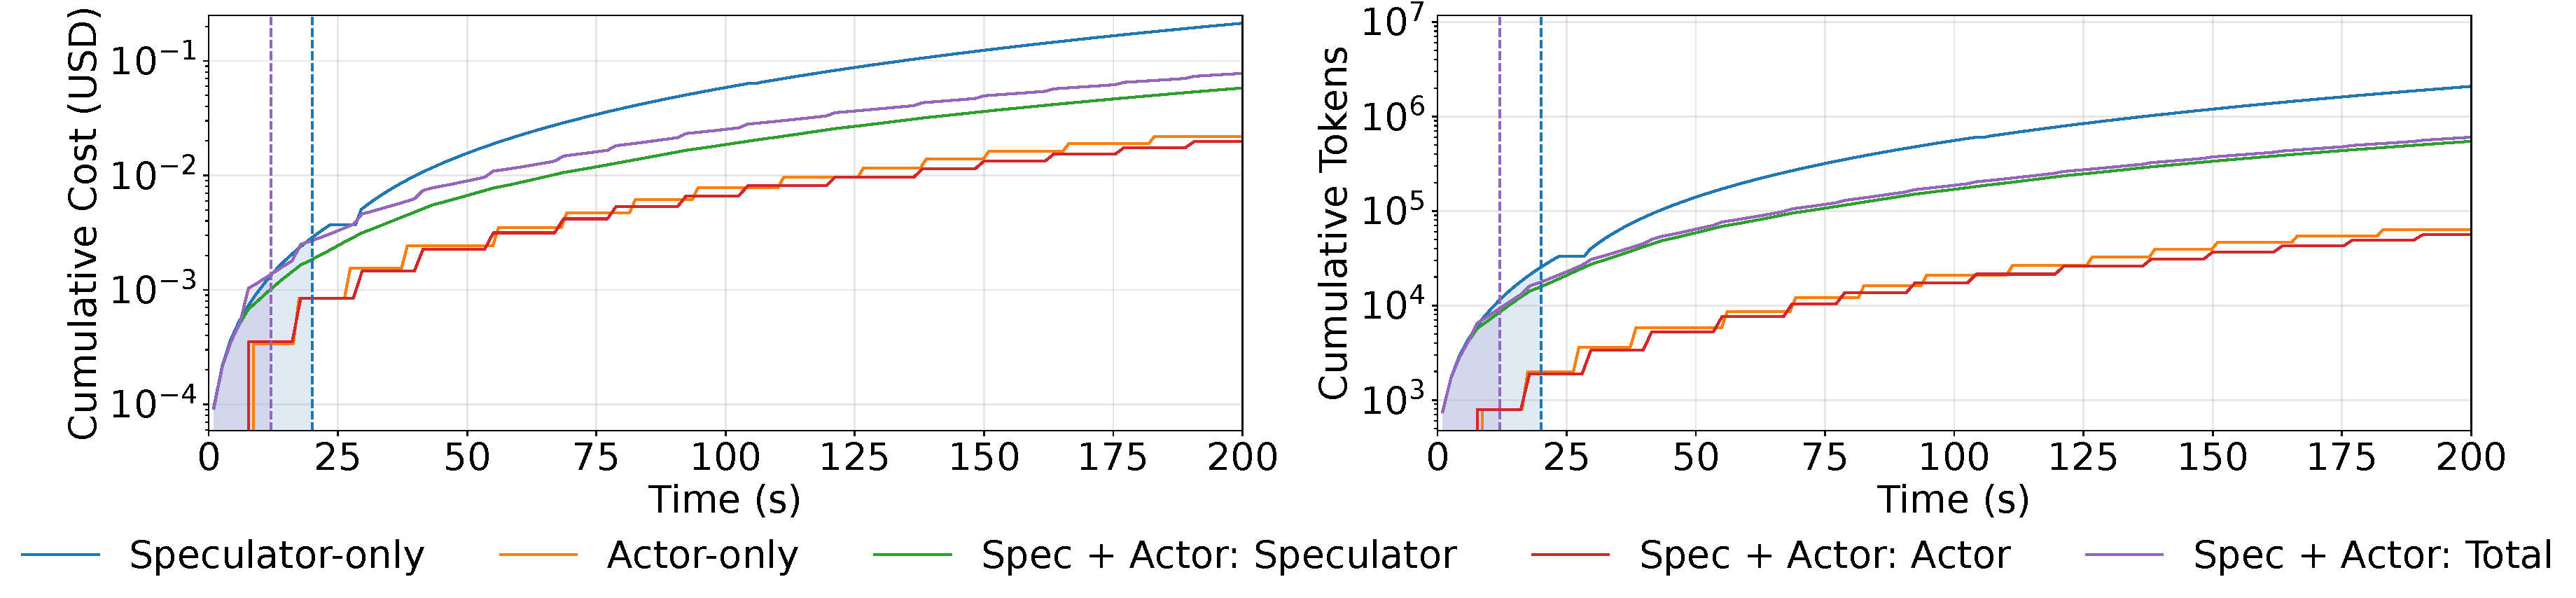
\includegraphics[width=\linewidth]{figures/os_tuning/cost.pdf}
%   \caption{\textbf{Cumulative token usage and cost over time.}
%   The left and right plots show the cumulative cost (USD) and total tokens used, respectively, for all three configurations.
%   The vertical lines mark the observed convergence point for each system. The Actor-only model converges at 200s}
%   \label{fig:costs}
% \end{figure*}


% \begin{table*}[ht]
% \centering
% \caption{Cumulative tokens and cost (in cents) at selected time marks. While Speculation incurs higher instantaneous costs, its rapid convergence (bolded) prevents long-term resource waste compared to the slower Actor-only baseline.}
% \label{tab:costs}
% \begin{tabular}{lrrrrrr}
% \toprule
% & \multicolumn{2}{c}{Actor-only} & \multicolumn{2}{c}{Speculator-only} & \multicolumn{2}{c}{Actor+Speculator (Total)} \\
% \cmidrule(lr){2-3}\cmidrule(lr){4-5}\cmidrule(lr){6-7}
% \textbf{Elapsed Time} & \textbf{Tokens} & \textbf{Cost (cents)} & \textbf{Tokens} & \textbf{Cost (cents)} & \textbf{Tokens} & \textbf{Cost (cents)} \\
% \midrule
% Base Prompt  & 744   & 0.02 & 690 & 0.01 & 1434 & 0.03 \\
% \textbf{\textcolor{mypurple}{13s}} 
%   & 1,216 & 0.05 & 14,973 & 0.18 
%   & \textbf{\textcolor{mypurple}{12,135}} 
%   & \textbf{\textcolor{mypurple}{0.17}} \\
% \textbf{\textcolor{myblue}{20s}} 
%   & 2,211 & 0.09 
%   & \textbf{\textcolor{myblue}{27,654}} 
%   & \textbf{\textcolor{myblue}{0.34}} 
%   & 20,504 & 0.31 \\
% 30s & 3,631   & 0.15 & 45,768 & 0.57 & 32,459 & 0.48 \\
% 60s & 8,581   & 0.35 & 205,794  & 2.24 & 84,568 & 1.18 \\
% 120s  & 26,398 & 0.96 & 778,253  & 8.12 & 261,855  & 3.53 \\
% \textbf{\textcolor{myred}{200s}} 
%   & \textbf{\textcolor{myred}{63,376}} 
%   & \textbf{\textcolor{myred}{2.18}} 
%   & 2,099,894 & 21.5 & 607,877 & 7.83 \\
% \bottomrule
% \end{tabular}
% \end{table*}

% \noindent \textbf{Impact of Context Strategy on Cost.} 
% While the Speculator operates at high frequency, the cost overhead is mitigated by the history compression mechanism described in \S\ref{app:history_os}. 
% In the combined system, the expensive Actor model reads only a compressed summary of the Speculator's many steps, rather than the raw verbose logs. 
% This keeps the prompt size for the Actor relatively stable compared to a linear growth of uncompressed history. 
% As a result, the cost difference between the Actor-only and Speculator+Actor systems is driven primarily by the number of Speculator calls, rather than an explosion in context size per call.

% As illustrated in Figure~\ref{fig:costs} and detailed in Table~\ref{tab:costs}, the high frequency of the Speculator leads to rapid growth in token consumption and cost. 
% In practice, however, this growth is bounded by the system's fast convergence. 
% The combined Actor-Speculator system converges in approximately 13 seconds, while the Speculator-only system converges in 20 seconds. The Actor-only system converges after 200 seconds. 
% Once an optimal state is reached, the tuning process concludes, rendering the potential for long-term exponential cost negligible in this context. Several optimization strategies, like truncating the context to a fixed window or disabling exploration after convergence, could further mitigate token growth but are left for future work.

\subsubsection{Speculative Reaction Time Benefits}
\label{app:speculative-mitigation}

To provide a targeted example of how speculation mitigates transient performance loss, we conducted a controlled experiment. In this scenario, the system is deliberately perturbed at time $t_0$ by setting the \ttt{min\_granularity} parameter to a highly suboptimal value (10 ms). We then compare the system's recovery under two configurations: the Actor-Speculator system and an Actor-Only baseline, which replays only the actions proposed by the Actor from the full Actor-Speculator trace.

\begin{figure}[h!]
  \centering
  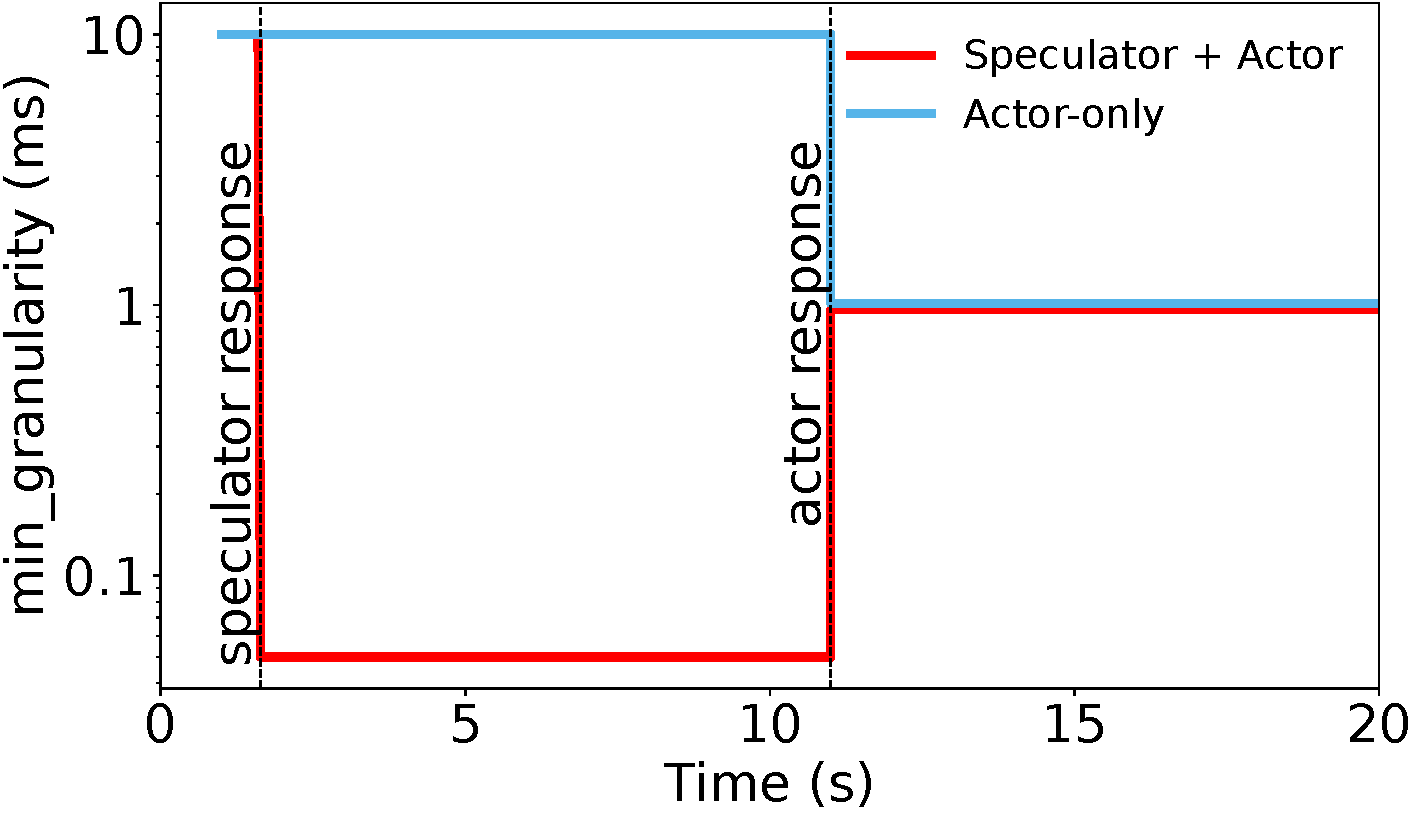
\includegraphics[width=0.6\linewidth]{figures/os_tuning/comparison.pdf}
  \caption{A controlled experiment showing the system's step response after a manual perturbation at $t=0$. The \textbf{Actor-Speculator} system corrects the poor setting within a second, while the \textbf{Actor-only} system must wait over 10 seconds for its next decision cycle. The quantitative results of this experiment are summarized in Figure~\ref{fig:os-speculation} (Right) in the main text.}
  \label{fig:os-reaction-appendix}
\end{figure}

As shown in Figure~\ref{fig:os-reaction-appendix}, the Actor-Speculator system reacts almost instantly. The fast Speculator, seeing the immediate performance degradation, applies a corrective action that brings the system back to an efficient state in about one second. In contrast, the Actor-Only system is forced to endure the poor performance for over 10 seconds, as it must wait for the slower Actor to complete its deliberation cycle before it can act.
The performance gap shown in the plot is quantified in the main text (Figure~\ref{fig:os-speculation}, Right).

\newpage 
\section{Cost--Latency Tradeoff}
\label{app:cost-latency}
% We study the cost--latency tradeoff of Speculative Action, where at each time step the Speculator could launch multiple speculative branches in parallel, each proposing a candidate next tool-call. 
\subsection{Breadth-focused speculation details}
Algorithm 1 launches $k$ parallel speculative branches at any step $t\in\{1,\dots,T-1\}$, which is then immediately followed  with an API call. We assume each branch independently produces the correct next call with probability $p$. Let
\[
p(k) := \Pr(\text{at least one branch is correct}) 
= 1 - (1-p)^k.
\]

We assume the latency of a speculative call is $\mathrm{Exp}(\alpha)$, and the latency of a real API call is $\mathrm{Exp}(\beta)$ with $\beta < \alpha$. Let $c$ denote the cost per unit time for both speculation and real API work. Let
\[
\E[T_{\mathrm{spec}}],\quad \E[M_{\mathrm{spec}}]
\]
denote the expected latency and cost under Algorithm~1 (1 step breadth speculation), and similarly let $(T_{\mathrm{seq}},M_{\mathrm{seq}})$ denote the sequential process with no speculation.

\vspace{3pt}
\begin{theorem}[Cost--Latency Tradeoff for Breadth Speculation]
\label{thm:cost-latency-tradeoff}
Under the setup above,
\begin{align*}
    \frac{E[T_{\mathrm{seq}} - T_{\mathrm{spec}}]}{E[T_{\mathrm{seq}}]}
    \;=\;&\frac{1}{T}\frac{\alpha}{\alpha+\beta}\left[\frac{(T-1)p(k)}{1+p(k)}+\frac{p(k)^2}{(1+p(k))^2} - \frac{p(k)^2}{(1+p(k))^2}(-p(k))^{T-1}\right]\\
    &\xrightarrow{\;\;T\to\infty\;\;}
    \frac{p(k)}{1+p(k)}\cdot\frac{\alpha}{\alpha+\beta}
\end{align*}

For cost, letting $\tilde{k}$ denote the number of \emph{distinct} actions produced across the $k$ speculative branches,
\begin{align*}
    \frac{\E[M_{\mathrm{spec}} - M_{\mathrm{seq}}]}{\E[M_{\mathrm{seq}}]}
    &=\tilde{k}
    -\frac{1}{T}\left(\tilde{k}+\frac{\alpha}{\alpha+\beta}\right)
    \left[
        \frac{(T-1)p(k)}{1+p(k)}
        +\frac{p(k)^2}{(1+p(k))^2}
        -\frac{p(k)^2}{(1+p(k))^2}(-p(k))^{T-1}
    \right]
    \\
    &\xrightarrow{T\to\infty}
    \tilde{k}
    -
    \left(\tilde{k}+\frac{\alpha}{\alpha+\beta}\right)
    \frac{p(k)}{1+p(k)}.
\end{align*}
Note that $\tilde{k}$ is possibly different from $k$ because the $k$ independent speculations might have duplications, in which case we kill the duplicated speculation processes.
\end{theorem}

\begin{proof}
 The proof of the time savings ratio is given in Appendix~\ref{app:proof}. For cost, we have
    \[M_{seq} \propto \frac{T}{\beta}\]
    \[M_{spec} \propto \frac{T}{\beta}(\tilde{k}+1) - S_{T-1}\left(\tilde{k}\frac{1}{\beta} +\frac{\alpha}{\beta(\alpha+\beta)}\right)\]
    where the speculative expression is due to each hit by time step $T-1$ will result in (i) the cached next step not having a speculative window, hence does not launch any speculations (ii) over counting hit action's generation time with execution time.

    Plug in expressions we obtained from Appendix~\ref{app:proof}, we get the expression desired.
\end{proof}

% \paragraph{Interpretation.}
% In the above analysis, we can see that the cost ratio $\left(\tilde{k}+\frac{\alpha}{\alpha+\beta}\right)
%     \frac{p(k)}{1+p(k)}$ and latency ratio $\frac{p(k)}{1+p(k)}\cdot\frac{\alpha}{\alpha+\beta}$, both governed by $p(k)$ with respect to a change in $k$, poses a fundamental tradeoff between the latency gains and the cost induced with extra calls.

% \begin{remark}
%     Note that the above speculation framework could be interpreted as a breadth-focused search, where each speculation is immediately followed by a real API call, hence with depth 1. In the next section, we analyze the other extreme where we do depth-focused search.
% \end{remark}


\subsection{Additional Empirical Results}
\label{app:additional-empiricals}
% \subsubsection{Chess}
% \begin{table}[h!]
% \centering
% \small
% \setlength{\tabcolsep}{4pt}
% \begin{tabular}{c|c|cccc}
% \hline
% \textbf{Number of Speculations} & \textbf{Metric} & 20 steps & 30 steps & 40 steps & 50 steps \\
% \hline
% 1 & Time Saved Percentage (\%) & 6.00 & 8.30 & 5.89 & 4.35 \\
%  Speculation & Extra Tokens used (\%) & 91.82 & 90.73 & 93.45 & 91.00 \\
% \hline
% 2 & Time Saved Percentage (\%) & 16.51 & 17.99 & 14.38 & 11.44 \\
%   Speculations& Extra Tokens used (\%) & 148.98 & 147.96 & 158.69 & 161.26 \\
% \hline
% 3 & Time Saved Percentage (\%) & 28.11 & 30.96 & 23.52 & 19.32 \\
% Speculations  &Extra Tokens used (\%) & 171.64 & 166.06 & 191.26 & 192.13 \\
% \hline
% Confidence-based & Time Saved Percentage (\%) & \textbf{21.97} & \textbf{24.53} & \textbf{18.95} & \textbf{16.18} \\
%  selective launch & Extra Tokens used (\%) & \textbf{90.97} & \textbf{90.11} & \textbf{87.14} & \textbf{84.89} \\
% \hline
% \end{tabular}
% \end{table}

% \begin{figure}[h]
%     \centering
%     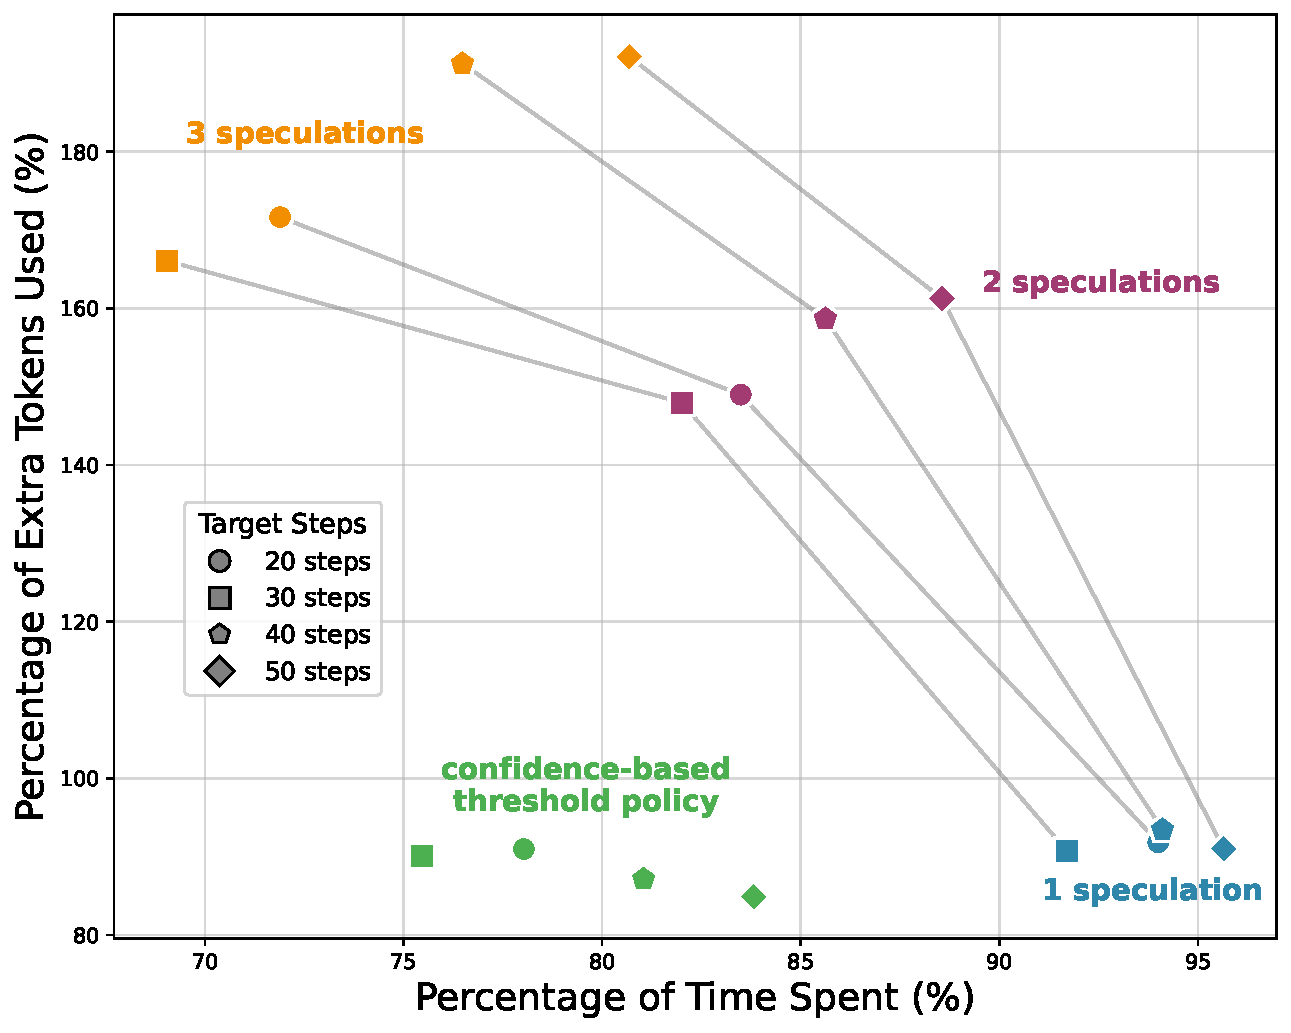
\includegraphics[width=0.7\linewidth]{figures/chess/plot_with_confidence.pdf}
%     \caption{Cost-latency tradeoff across different speculation numbers. With confidence prediction heuristic described above, we are able to achieve lowest cost with comparable time save as 3 predictions, outperforming 2 and 1 predictions.}
%     \label{fig:tradeoff}
% \end{figure}

% \paragraph{Trade-off between Time Saved and Token Cost.} In addition to time savings, we also measure the additional token cost of parallel speculation. We track this using the metric \textbf{extra token percentage}: $(M_{speculative} -M_{sequantial})/{M_{sequential}}$. Figure~\ref{fig:tradeoff} shows the trade-off between time saved and token cost for each number of predictions. We observe that the extra token percentage increases as the number of predictions increases, while the time saved percentage also increases, creating a clear trade-off. Additionally, we observe through the 1,2,3 prediction pattern that there is a non-linear increase cost increase ratio, as consistent with Theorem~\ref{thm:cost-latency-tradeoff}: as $k$ increases, the coefficient $1/1+p(k)$ decreases, thus creating a non-linear dependence.


\subsubsection{E-commerce}

\paragraph{Trade-off between Prediction Accuracy and Cost.}
The time cost in Figure~\ref{fig:time_acc} consists of latency (Time to First Token) and output response time. The dashed vertical line represents the average user typing time, estimated at 40 words per minute. At this threshold, the multi-agent setting achieves approximately 34\% prediction accuracy, meaning that in over one-third of cases the agent can return an immediate response without waiting for API execution. This demonstrates that speculation can transform user experience from perceptibly laggy to effectively real-time in tool-heavy environments.

\begin{figure}[H]
  \centering
  \resizebox{0.8\textwidth}{!}{%
      \begin{subfigure}[t]{0.48\textwidth}
        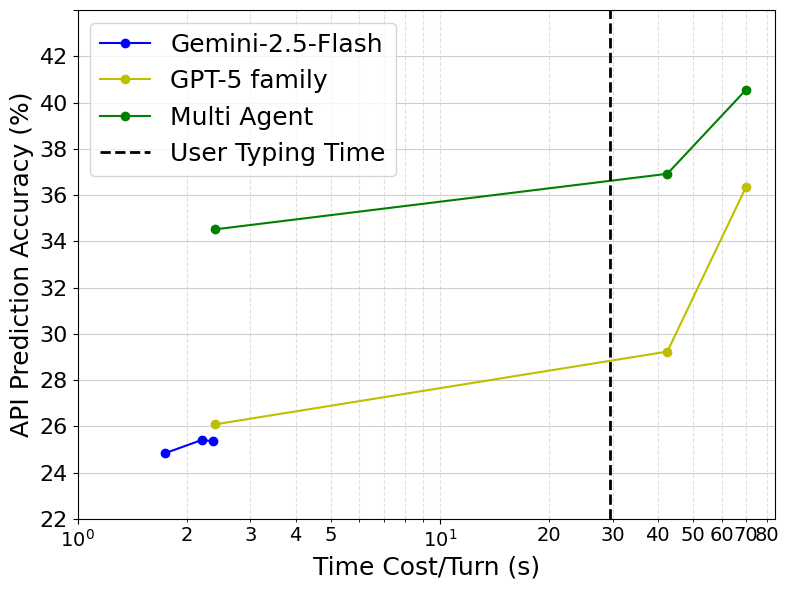
\includegraphics[width=\linewidth]{figures/ecommerce/time_accuracy.png}
        \caption{}
        \label{fig:time_acc}
      \end{subfigure}
      \hspace{0.05\textwidth} 
      \begin{subfigure}[t]{0.48\textwidth}
        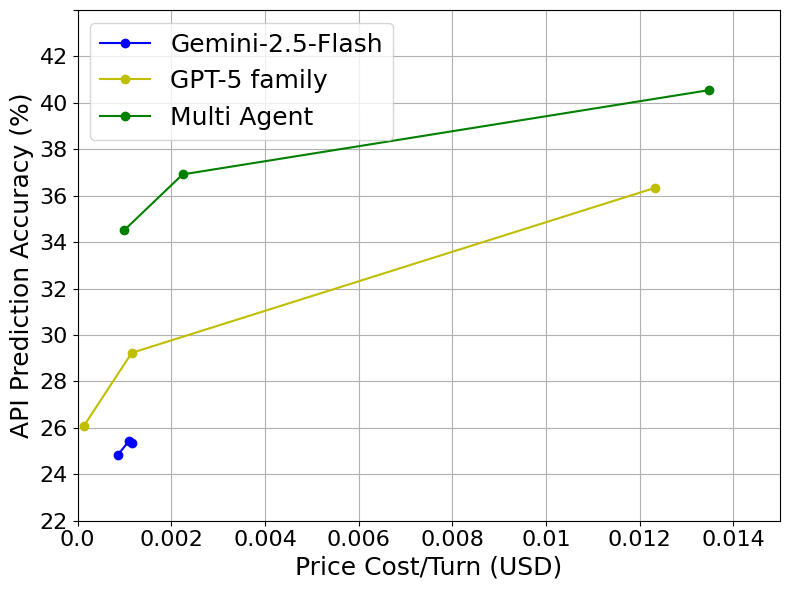
\includegraphics[width=\linewidth]{figures/ecommerce/price_accuracy.png}
        \caption{}
        \label{fig:price_acc}
      \end{subfigure}
  }
  \caption{\textbf{Prediction Accuracy against Speculator's Cost across different models.} (a) Accuracy–Speculator time cost trade-off across models. The dashed line shows average user typing time. (d) Accuracy–Speculator price trade-off across models, reflecting the monetary cost of speculative execution.}
  \vspace{-1em}
\end{figure}


\subsubsection{OS hyperparameter tuning}

\begin{figure*}[h]
  \centering
  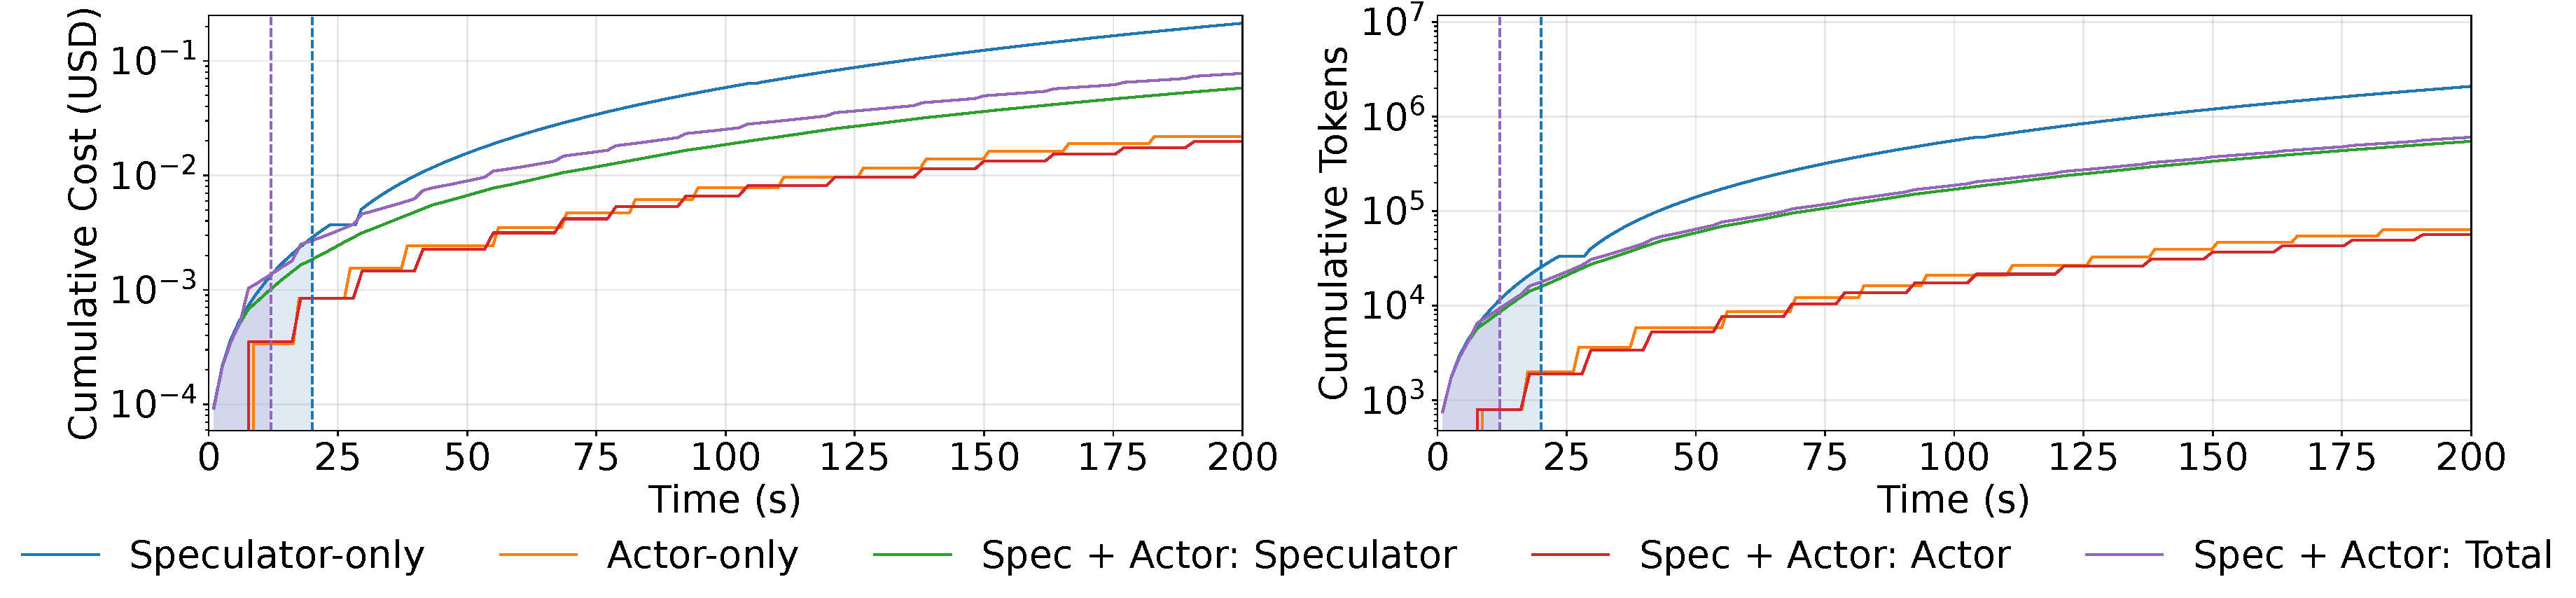
\includegraphics[width=\linewidth]{figures/os_tuning/cost.pdf}
  \caption{\textbf{Cumulative token usage and cost over time.}
  The left and right plots show the cumulative cost (USD) and total tokens used, respectively, for all three configurations.
  The vertical lines mark the observed convergence point for each system. The Actor-only model converges at 200s}
  \label{fig:costs}
\end{figure*}


\begin{table*}[ht]
\centering
\caption{Cumulative tokens and cost (in cents) at selected time marks. While Speculation incurs higher instantaneous costs, its rapid convergence (bolded) prevents long-term resource waste compared to the slower Actor-only baseline.}
\label{tab:costs}
\begin{tabular}{lrrrrrr}
\toprule
& \multicolumn{2}{c}{Actor-only} & \multicolumn{2}{c}{Speculator-only} & \multicolumn{2}{c}{Actor+Speculator (Total)} \\
\cmidrule(lr){2-3}\cmidrule(lr){4-5}\cmidrule(lr){6-7}
\textbf{Elapsed Time} & \textbf{Tokens} & \textbf{Cost (cents)} & \textbf{Tokens} & \textbf{Cost (cents)} & \textbf{Tokens} & \textbf{Cost (cents)} \\
\midrule
Base Prompt  & 744   & 0.02 & 690 & 0.01 & 1434 & 0.03 \\
\textbf{\textcolor{mypurple}{13s}} 
  & 1,216 & 0.05 & 14,973 & 0.18 
  & \textbf{\textcolor{mypurple}{12,135}} 
  & \textbf{\textcolor{mypurple}{0.17}} \\
\textbf{\textcolor{myblue}{20s}} 
  & 2,211 & 0.09 
  & \textbf{\textcolor{myblue}{27,654}} 
  & \textbf{\textcolor{myblue}{0.34}} 
  & 20,504 & 0.31 \\
30s & 3,631   & 0.15 & 45,768 & 0.57 & 32,459 & 0.48 \\
60s & 8,581   & 0.35 & 205,794  & 2.24 & 84,568 & 1.18 \\
120s  & 26,398 & 0.96 & 778,253  & 8.12 & 261,855  & 3.53 \\
\textbf{\textcolor{myred}{200s}} 
  & \textbf{\textcolor{myred}{63,376}} 
  & \textbf{\textcolor{myred}{2.18}} 
  & 2,099,894 & 21.5 & 607,877 & 7.83 \\
\bottomrule
\end{tabular}
\caption{}
\label{tab:os}
\end{table*}

\noindent \textbf{Impact of Context Strategy on Cost.} 
While the Speculator operates at high frequency, the cost overhead is mitigated by the history compression mechanism described in \S\ref{app:history_os}. 
In the combined system, the expensive Actor model reads only a compressed summary of the Speculator's many steps, rather than the raw verbose logs. 
This keeps the prompt size for the Actor relatively stable compared to a linear growth of uncompressed history. 
As a result, the cost difference between the Actor-only and Speculator+Actor systems is driven primarily by the number of Speculator calls, rather than an explosion in context size per call.

As illustrated in Figure~\ref{fig:costs} and detailed in Table~\ref{tab:costs}, the high frequency of the Speculator leads to rapid growth in token consumption and cost. 
In practice, however, this growth is bounded by the system's fast convergence. 
The combined Actor-Speculator system converges in approximately 13 seconds, while the Speculator-only system converges in 20 seconds. The Actor-only system converges after 200 seconds. 
Once an optimal state is reached, the tuning process concludes, rendering the potential for long-term exponential cost negligible in this context. Several optimization strategies, like truncating the context to a fixed window or disabling exploration after convergence, could further mitigate token growth but are left for future work.

\subsection{Confidence-Aware Speculation}

We formalize the branch selection problem introduced in
Section~\ref{subsec:dynamic-speculation}.

\paragraph{Model.}
Fix a horizon $T$ and an integer $k \ge 1$.
At each epoch $t$, the system is in mode $z_t \in \{0,1\}$:
\begin{itemize}
    \item $z_t = 0$: a speculation window is available,
    \item $z_t = 1$: a cached correct action must be executed (no speculation).
\end{itemize}

Let $a$ and $b$ denote the actor and speculator latencies, respectively, and define the latency gain
\[
\ell := a - b > 0,
\]
which is collected only at epochs with $z_t = 1$.

\paragraph{Accuracy process.}
At epochs with $z_t = 0$, an accuracy vector
$\mathbf P_t = (P_t^1,\dots,P_t^k) \in [0,1]^k$
is realized and observed.
Assume $\mathbf P_t \sim F_t$ independently across $t$,
where the distribution $F_t$ may vary over time.

Given a realization $\mathbf p$, let
$p^{(1)} \ge \dots \ge p^{(k)}$
denote the sorted coordinates.

\paragraph{Action and hit probability.}
At $z_t = 0$, the agent chooses $m_t \in \{0,\dots,k\}$,
launching the top $m_t$ branches at cost $c m_t$.
The probability of obtaining a cached action is
\[
q(m;\mathbf p)
=
1 - \prod_{j=1}^{m} (1 - p^{(j)}),
\qquad
q(0;\mathbf p) = 0.
\]

\paragraph{Mode transition.}
If $z_t = 1$, then $z_{t+1} = 0$ deterministically.
If $z_t = 0$ and action $m$ is chosen,
\[
z_{t+1} =
\begin{cases}
1, & \text{w.p. } q(m;\mathbf P_t), \\
0, & \text{w.p. } 1 - q(m;\mathbf P_t).
\end{cases}
\]

\paragraph{Reward.}
The per-epoch reward is
\[
R_t =
\begin{cases}
\ell, & z_t = 1, \\
- c m_t, & z_t = 0.
\end{cases}
\]
The objective is to maximize
$\mathbb E\!\left[\sum_{t=1}^T R_t\right]$.


We then present the proof to the first part (general non-stationary) of Theorem~\ref{thm:dynamic}.

\begin{proof}
Let $V_t^{(z)}$ denote the optimal expected total reward from epochs
$t,\dots,T$ given mode $z_t=z$,
with terminal conditions
$V_{T+1}^{(0)} = V_{T+1}^{(1)} = 0$.

By standard dynamic programming arguments,
the Bellman equations are
\begin{align}
V_t^{(1)} &= \ell + V_{t+1}^{(0)}, \label{eq:bellman1} \\
V_t^{(0)} &=
\mathbb E_{\mathbf P \sim F_t}
\Big[
\max_{m \in \{0,\dots,k\}}
\big\{
- c m
+ q(m;\mathbf P)\,V_{t+1}^{(1)}
+ (1-q(m;\mathbf P))\,V_{t+1}^{(0)}
\big\}
\Big].
\label{eq:bellman0}
\end{align}

Define the continuation gap
\[
\Delta_t := V_{t+1}^{(1)} - V_{t+1}^{(0)}.
\]

Substituting \eqref{eq:bellman1} into \eqref{eq:bellman0} yields
\[
V_t^{(0)}
=
V_{t+1}^{(0)}
+
\mathbb E_{\mathbf P \sim F_t}
\Big[
\max_m
\{ q(m;\mathbf P)\,\Delta_t - c m \}
\Big].
\]

Hence, conditional on observing $\mathbf p$ at epoch $t$,
the optimal decision maximizes
\[
q(m;\mathbf p)\,\Delta_t - c m,
\]
establishing the stated policy.

Finally, using
\[
\Delta_t
=
V_{t+1}^{(1)} - V_{t+1}^{(0)}
=
\ell + V_{t+2}^{(0)} - V_{t+1}^{(0)},
\]
and substituting the expression for $V_{t+1}^{(0)}$
gives the scalar recursion
\[
\Delta_t
=
\ell
-
\mathbb E_{\mathbf P \sim F_{t+1}}
\Big[
\max_m \{ q(m;\mathbf P)\,\Delta_{t+1} - c m \}
\Big],
\]
with terminal condition $\Delta_T = 0$ (or equivalently, $\Delta_{T-1} = \ell$).
\end{proof}

% \begin{remark}[Mean-only approximation]
% Suppose only the mean accuracy vectors
% $\mu_t := \mathbb E_{F_t}[\mathbf P_t]$
% are available.
% Let $\mu_t^{(1)} \ge \dots \ge \mu_t^{(k)}$ denote the sorted coordinates,
% and define
% \[
% \bar q_t(m)
% =
% 1 - \prod_{j=1}^{m} (1 - \mu_t^{(j)}).
% \]

% Replacing the expectation in the scalar recursion by this
% certainty-equivalent hit probability yields
% \[
% \tilde\Delta_T = \ell,
% \qquad
% \tilde\Delta_t
% =
% \ell
% -
% \max_{m \in \{0,\dots,k\}}
% \{ \bar q_{t+1}(m)\,\tilde\Delta_{t+1} - c m \}.
% \]

% The resulting implementable policy is
% \[
% \tilde m_t(\mathbf p)
% \in
% \arg\max_{m}
% \{ q(m;\mathbf p)\,\tilde\Delta_t - c m \}.
% \]

% This approximation is exact if $F_t$ is degenerate at its mean,
% and otherwise serves as a computationally light surrogate.
% \end{remark}
% \begin{lemma}[Marginal-threshold form of the stationary policy]
% Fix a constant $\Delta^\star>0$ and per-branch cost $c>0$.
% Given a realization $\mathbf p=(p^1,\dots,p^k)$, let
% $p^{(1)}\ge \cdots \ge p^{(k)}$ be the sorted probabilities and define
% \[
% q(m;\mathbf p) := 1-\prod_{j=1}^{m}(1-p^{(j)}), \qquad q(0;\mathbf p)=0,
% \]
% and the incremental hit probability
% \[
% \delta q(m;\mathbf p) := q(m+1;\mathbf p)-q(m;\mathbf p)
% = \left(\prod_{j=1}^{m}(1-p^{(j)})\right)p^{(m+1)}.
% \]
% Then any maximizer
% \[
% m^\star(\mathbf p)\in\arg\max_{m\in\{0,\dots,k\}}\{q(m;\mathbf p)\Delta^\star-cm\}
% \]
% satisfies the marginal cutoff condition
% \[
% \Delta^\star \cdot \delta q(m;\mathbf p)\ \ge\ c \quad \text{for all } m<m^\star(\mathbf p),
% \qquad
% \Delta^\star \cdot \delta q(m;\mathbf p)\ \le\ c \quad \text{for all } m\ge m^\star(\mathbf p).
% \]
% Equivalently, $m^\star(\mathbf p)$ can be obtained by the greedy rule:
% starting from $m=0$, repeatedly add the next-best branch $(m+1)$ while
% $\Delta^\star \cdot \delta q(m;\mathbf p)\ge c$, and stop otherwise.
% \end{lemma}

% \naimeng{The other modeling: suppose this is infinite horizon but optimal stopping: each step there is q probability to exit.}
We then formally describe the stationary average reward corollary. 
\begin{corollary}[Stationary infinite-horizon average-reward policy]
Assume the nonstationary model becomes stationary:
\begin{itemize}
    \item $\mathbf P_t \sim F$ i.i.d.\ across $t$,
    \item the hit probability $q(m;\mathbf p)$ and cost $c$ are time-invariant,
    \item the objective is to maximize long-run average reward.
\end{itemize}

Let $\bar q(m) := \mathbb E_{\mathbf P \sim F}[q(m;\mathbf P)]$ denote
the expected hit probability when launching $m$ branches.

Then the optimal average reward $g^\star$ satisfies
\[
g^\star
=
\max_{m \in \{0,\dots,k\}}
\frac{\bar q(m)\,\ell - c m}{1 + \bar q(m)}.
\]

Define
\[
\Delta^\star := \ell - g^\star.
\]

Then an optimal stationary policy at a speculation window is
\[
m^\star(\mathbf p)
\in
\arg\max_{m \in \{0,\dots,k\}}
\{ q(m;\mathbf p)\,\Delta^\star - c m \}.
\]

In particular, the optimal policy mapping (the scalar $\Delta^\star$) is time homogeneous.
\end{corollary}

\begin{proof}
Fix $\Delta^\star>0$. Conditional on observing $\mathbf p$ at a speculation window, the stationary one-step objective is
\[
f(m;\mathbf p) := q(m;\mathbf p)\,\Delta^\star - c m,
\qquad m\in\{0,1,\dots,k\}.
\]
The first display in the corollary is exactly the definition of $m^\star(\mathbf p)$ as any maximizer of $f(m;\mathbf p)$.

To show the greedy marginal-threshold form, note that for sorted confidences
$p^{(1)}\ge\cdots\ge p^{(k)}$,
\[
q(m;\mathbf p)=1-\prod_{j=1}^{m}(1-p^{(j)}),
\]
so the discrete marginal gain from adding the $(m+1)$-th branch is
\[
f(m+1;\mathbf p)-f(m;\mathbf p)
=\Delta^\star\bigl(q(m+1;\mathbf p)-q(m;\mathbf p)\bigr)-c
=\Delta^\star\,\delta q(m;\mathbf p)-c,
\]
where
\[
\delta q(m;\mathbf p)
:=q(m+1;\mathbf p)-q(m;\mathbf p)
=\Big(\prod_{j=1}^{m}(1-p^{(j)})\Big)p^{(m+1)}.
\]
Moreover, $\delta q(m;\mathbf p)$ is nonincreasing in $m$ (diminishing returns), since
$p^{(m+1)}$ is nonincreasing and the prefactor $\prod_{j=1}^{m}(1-p^{(j)})$ is nonincreasing in $m$.
Hence the increments $f(m+1;\mathbf p)-f(m;\mathbf p)$ are nonincreasing in $m$ as well.

Therefore there exists an index $m^\star(\mathbf p)$ such that
$f(m+1;\mathbf p)-f(m;\mathbf p)\ge 0$ for all $m<m^\star(\mathbf p)$ and
$f(m+1;\mathbf p)-f(m;\mathbf p)\le 0$ for all $m\ge m^\star(\mathbf p)$.
Equivalently,
\[
\Delta^\star \cdot \delta q(m;\mathbf p)\ge c \;\;\text{for } m<m^\star(\mathbf p),
\qquad
\Delta^\star \cdot \delta q(m;\mathbf p)\le c \;\;\text{for } m\ge m^\star(\mathbf p),
\]
which is precisely the greedy stopping rule stated in the corollary.
\end{proof}

% \subsubsection{Experimental result}
% % We implement the above heuristic with the chess environment and plot the cost-latency tradeoff
% We implement a threshold policy discussed above in the chess environment. We use the same GPT5 model as the predictor. As shown in figure~\ref{fig:tradeoff}, our policy achieves lowest cost measured by extra tokens used, while achieving latency reduction exceeding both 1 and 2 prediction branchings, falling just short (less than $5\%$) of the latency reduction achieved by launching 3 speculations per step. 



% \subsection{Heuristic Policy for Dynamic Speculation Decisions}

% We now consider a more realistic setting in which, at each step, we observe a per-speculation confidence estimate. Suppose that launching a real API costs $a$ time units, a speculative call costs $b<a$, and each step the system produces $k$ speculative candidates with correctness probabilities $\{p_i^1,\dots,p_i^k\}$.

% Let $r$ and $c$ be the weights placed on latency and monetary cost, respectively, so that we maximize
% \[
% \max_{\pi} \; r\cdot\mathrm{latency} + c\cdot\mathrm{cost}.
% \]

% For a single speculation with correctness probability $p_i$, the decision is whether to \emph{accept} (continue unrolling this speculative branch) or \emph{reject} (discard it and continue sequentially). Let $V(i)$ be the optimal value-to-go at token index $i$.

% If we \textbf{accept} the speculation, the expected one-step reward is
% \begin{align*}
% A(i)
% &=
% p_i\bigl[ r b + c(b+a) + r a + c a + V(i+2)\bigr]
% +
% (1-p_i)\bigl[r a + 2c a + V(i+1)\bigr]
% \\
% &=
% p_i\bigl[ r b + c(b+a) + r a + c a + V(i+2)\bigr]
% + (1-p_i)\bigl[r a + 2c a + V(i+1)\bigr].
% \end{align*}

% If instead we \textbf{reject}, the expected reward is simply
% \[
% R(i) = r a + c a + V(i+1).
% \]

% We propose a simple heuristic: treat all future timesteps as if their speculation correctness probability is the baseline value $p$. Under this approximation the dynamic program becomes stationary, and for long horizons the value function becomes approximately linear, enabling a closed-form threshold policy.

% \subsection{Long-Horizon Approximation and Closed-Form Threshold Policy}



\subsection{Depth focused search}
In the most general setting, a policy may choose both (1) how many parallel speculative branches to launch, and (2) how “deep” to unroll each speculative branch before initiating a real API call. Analyzing the optimal policy in this full space is highly non-trivial due to the branching structure of the execution tree.

To build intuition, we analyze two extrema regimes:
(1) a \emph{breadth-focused} regime, where at each step we launch $k$ parallel speculations and immediately follow each with an API call, and  
(2) a \emph{depth-focused} regime, where execution follows a single branch as far as speculation and real API calls allow. These two settings correspond to simplified extremes of the decision space, providing interpretable analytic characterizations of the cost--latency tradeoff.

We analyzed the first in the previous section, and now analyze the opposite extreme: a depth-focused strategy. Under this policy, whenever either a speculative or real API call returns, the system launches \emph{one} new real call and \emph{one} speculation on top of that branch. If the real API result is inconsistent with the corresponding speculative guess, all descendants of that speculation are discarded. Let $p$ be the per-step correctness probability of a speculative guess.

Assume for simplicity that the real API call latency is deterministically $a$ and a speculative call latency is $b<a$.

\begin{theorem}[Cost--Latency Tradeoff for Depth Speculation]
Let $p$ be the probability that a speculation is correct at each step. Then under the depth-focused policy described above,
\[
    \frac{\E[T_{\mathrm{seq}} - T_{\mathrm{spec}}]}{\E[T_{\mathrm{seq}}]}
    = \frac{T-1}{T} \, p \Bigl(1 - \frac{b}{a}\Bigr),
\]
and the expected cost satisfies
\[
    \frac{\E[M_{\mathrm{spec}} - M_{\mathrm{seq}}]}{\E[M_{\mathrm{seq}}]}
    =
    \frac{T-1}{T}
    \frac{
        (1-p)\left[
            a\lfloor\tfrac{a}{b}\rfloor 
            - b\frac{(1+\lfloor\tfrac{a}{b}\rfloor)\lfloor\tfrac{a}{b}\rfloor}{2}
        \right]
        + p b\lfloor\frac{a}{b}\rfloor
    }{a}\approx\frac{T-1}{T}\left((1-p)\left(\frac{a}{2b}-\frac{1}{2}\right)+p\right)
\]
\label{thm:depth}
\end{theorem}

\begin{proof}
    We directly calculate the expected time cost of speculation execution as follows
    \[T_{spec} = a+ \sum_{s=0}^{T-1}\binom{T-1}{s}p^s(1-p)^{T-1-s}[sb+(T-1-s)a]\]
    Let 
\[
S \sim \mathrm{Binomial}(T-1, p),
\]
so that
\[
\mathbb{P}(S=s) = \binom{T-1}{s} p^s (1-p)^{T-1-s}, 
\quad s = 0, \dots, T-1.
\]

Then
\begin{align*}
&\sum_{s=0}^{T-1} \binom{T-1}{s} p^s (1-p)^{T-1-s}
\bigl[sb + (T-1-s)a\bigr] \\
&= \mathbb{E}\!\left[Sb + (T-1-S)a\right] \\
&= b\,\mathbb{E}[S] + a\,\mathbb{E}[T-1-S].
\end{align*}

Since
\[
\mathbb{E}[S] = (T-1)p,
\]
we obtain
\begin{align*}
b(T-1)p + a\bigl(T -1- (T-1)p\bigr)
&= a(T-1) + (T-1)p(b-a).
\end{align*}

Therefore,
\[T_{spec} = a+ 
\sum_{s=0}^{T-1} \binom{T-1}{s} p^s (1-p)^{T-1-s}
\bigl[sb + (T-s)a\bigr]
= aT + (T-1)p(b-a).
\]
Directly plug in $T_{seq} = aT$, we get the expression desired.

For cost, we know that with $(1-p)$ probability, speculation is inconsistent with true action, and the amount of tokens spent is from the branches that were spawn off before the correct action returns, that is
\begin{align*}
    \text{Token of this step} &= a+(a-b)+(a-2b)+\dots + \left(a-\lfloor\frac{a}{b}\rfloor b\right)\\
    &=a\cdot\left(\lfloor\frac{a}{b}\rfloor+1\right) - \frac{\left(1+\lfloor\frac{a}{b}\rfloor\right)\cdot\lfloor\frac{a}{b}\rfloor}{2}\cdot b
\end{align*}
With probability $p$, speculation matches with true action, in which case
\[\text{Token of this step} = a+ \lfloor\frac{a}{b}\rfloor b\]
Therefore
\begin{align*}
    M_{spec} &= a+ (T-1)\left[p\left(a+ \lfloor\frac{a}{b}\rfloor b\right)+(1-p)\left(a\cdot\left(\lfloor\frac{a}{b}\rfloor+1\right) - \frac{\left(1+\lfloor\frac{a}{b}\rfloor\right)\cdot\lfloor\frac{a}{b}\rfloor}{2}\cdot b\right)\right]
\end{align*}
\end{proof}

\paragraph{Interpretation.}
Note that compared to breadth speculation, Depth speculation produces speedups unbounded in $p$ coefficient (the coefficient in front for breadth is $\frac{1}{2}$ whereas for depth speculation this coefficient is 1). In terms of cost, depth speculation cost has highest order term $(1-p)(\frac{a}{2b}-\frac{1}{2})$. This is governed by how many speculations one can spawn off before the current action is returned. 




\end{document}
